
% ---------------------------- comment out when compiling the full document -------------------
\documentclass[12pt]{mytustyle}  % default square logo 
\usepackage{amssymb}
\usepackage{caption}
\usepackage{upgreek}
\usepackage{subfig}
\usepackage{enumitem}
\setlist[description]{leftmargin=0cm,labelindent=0cm}

\usepackage{packages/fancyhdr}% http://ctan.org/pkg/fancyhdr
\pagestyle{fancy}% Change page style to fancy
%\fancyhf{}% Clear header/footer
\fancyhead{}
\fancyhead[RO, LE]{Experimental results}
%\fancyfoot{}
%\fancyfoot[RO, LE]{\thepage}% \fancyfoot[R]{\thepage}
\renewcommand{\headrulewidth}{0.7pt}% Default \headrulewidth is 0.4pt
%\renewcommand{\footrulewidth}{0.7pt}% Default \footrulewidth is 0pt
%\rfoot{\thepage}

\begin{document}
\baselineskip=15pt
% ---------------------------------------------------------------------------------------------------------------


% ---------------------------------------------------------------------------------------------------------------
\chapter{Experimental results}
% ---------------------------------------------------------------------------------------------------------------

%Noise limitations
%
%Lab measurements
%
%Temperature and radiation limitations
%
%Transient current technique
%
%Charge - before and after irradiation
%
%compare with RD42 results
%
%Generation of trapping centres, reference KIT, Marok, Harris�
%
%IIa

This chapter contains the measurement results of data taken with diamond sensors. The description of measurement setup (section~\ref{sec:meassetup}) 
%and the experimental technique (section~\ref{sec:exptech}) 
is followed by applying experimental techniques and a discussion of results in order to find operational limitations in sections \ref{sec:noiselimit}, \ref{sec:templimit} and \ref{sec:radlimit}. The aim of the chapter is to compare the experimentally acquired data with the theory from the previous chapter. 

Diamond sensors are mainly used for two types of measurements: particle counting and spectroscopy. The first type of measurements depends on the sensor's efficiency -- the ability to detect all or at least a known percentage of particles/photons that hit it. The energy of the radiation is not so important; what bears the information is the rate and the spatial distribution. Here the radiation does not necessarily stop in the bulk, but rather continues its way. In spectroscopy, on the other hand, the idea is that a particle stops within the sensor, depositing all its energy, which is then measured via the freed charge carriers. The aim of the experiments described in this chapter is to 1) quantify the efficiency of the sCVD diamond in counting mode, 2) quantify the efficiency degradation with received radiation dose, 3) quantify the macroscopic effects on charge carrier behaviour with received radiation dose and 4) define limitations for its use in spectroscopy.

The results discussed here show that there are several limitations of the diamond as a measurement device. All of them need to be taken into account for the measurement device to perform reliably and stably. The first step is to build a setup that is insensitive to environmental interferences and minimises electrical noise in the system. The setup needs to be calibrated before use. Then, the measurement conditions have to be defined, such as the type of radiation and its flux. This allows us to estimate the lifetime of the detector and predict the longterm change of the signal. This change can then be accounted for when interpreting the output data. 






%\tableofcontents


% ---------------------------------------------------------------------------------------------------------------
%\clearpage
\section{Measurement setup}
\label{sec:meassetup}
% ---------------------------------------------------------------------------------------------------------------
As said in the introduction, in order to get reliable measurement results, great care has to go towards designing a measurement setup that minimises the noise in the measurements. In practice this often means using extensive amounts of aluminium foil and cardboard boxes. The foil is wrapped around the exposed parts of the system to shield it from external radio-frequency (RF) interferences. The boxes are usually just put on top of the setup to prevent the light from shining directly onto the sensors. There are of course more professional ways of doing it, but these two items are nevertheless always found in PhD students' labs.

The measurements using diamond and explained in these chapters were carried out using several setups, but there is a recurring theme to all of them. The measurement chain consists of three main parts: a diamond sensor, a signal preamplifier and a readout device, as seen in diagram~\ref{fig:ro-chain}. The signals propagating along the analogue chain (before being digitised by the readout device) are fast -- in the GHz bandwidth range --  and with low amplitudes, which gives rise to importance of RF shielding. Also, the connection between the carrier and the preamplifier has to be as short as possible to avoid capacitive signal losses in the transmission line. Finally, the system needs to be grounded properly.

\begin{figure}
\centering
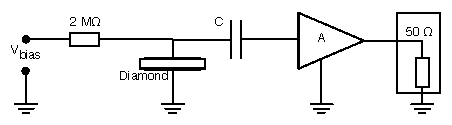
\includegraphics[width=0.8\textwidth]{plots/ro-chain}
\caption{Diagram of a diamond detector readout chain.}
\label{fig:ro-chain}
\end{figure}


\subsection{Preamplifiers}
\label{sec:preamps}
Two preamplifiers were used for the measurements, one sensitive to charge and the other to current. \emph{CIVIDEC Cx} (figure~\ref{fig:ampcx}) is a charge shaping amplifier. Its high SNR (low noise of 400~electrons and a reported gain of $\sim$8.2~mV/fC) makes it a good choice for spectroscopic measurements with diamond sensors. \emph{CIVIDEC C2} (figure~\ref{fig:ampc2}) is a fast current preamplifier with a 2~GHz bandwidth limit. It is used for TCT measurements because if its fast response and a good SNR. Both are embedded in an RF-tight aluminium box to reduce the noise pickup. Both have an AC coupled input and a 50~$\Upomega$ output.

\begin{figure}[!t]
%\centering
\begin{tabular}{cccc}
\subfloat[Cx charge shaping preamplifier]{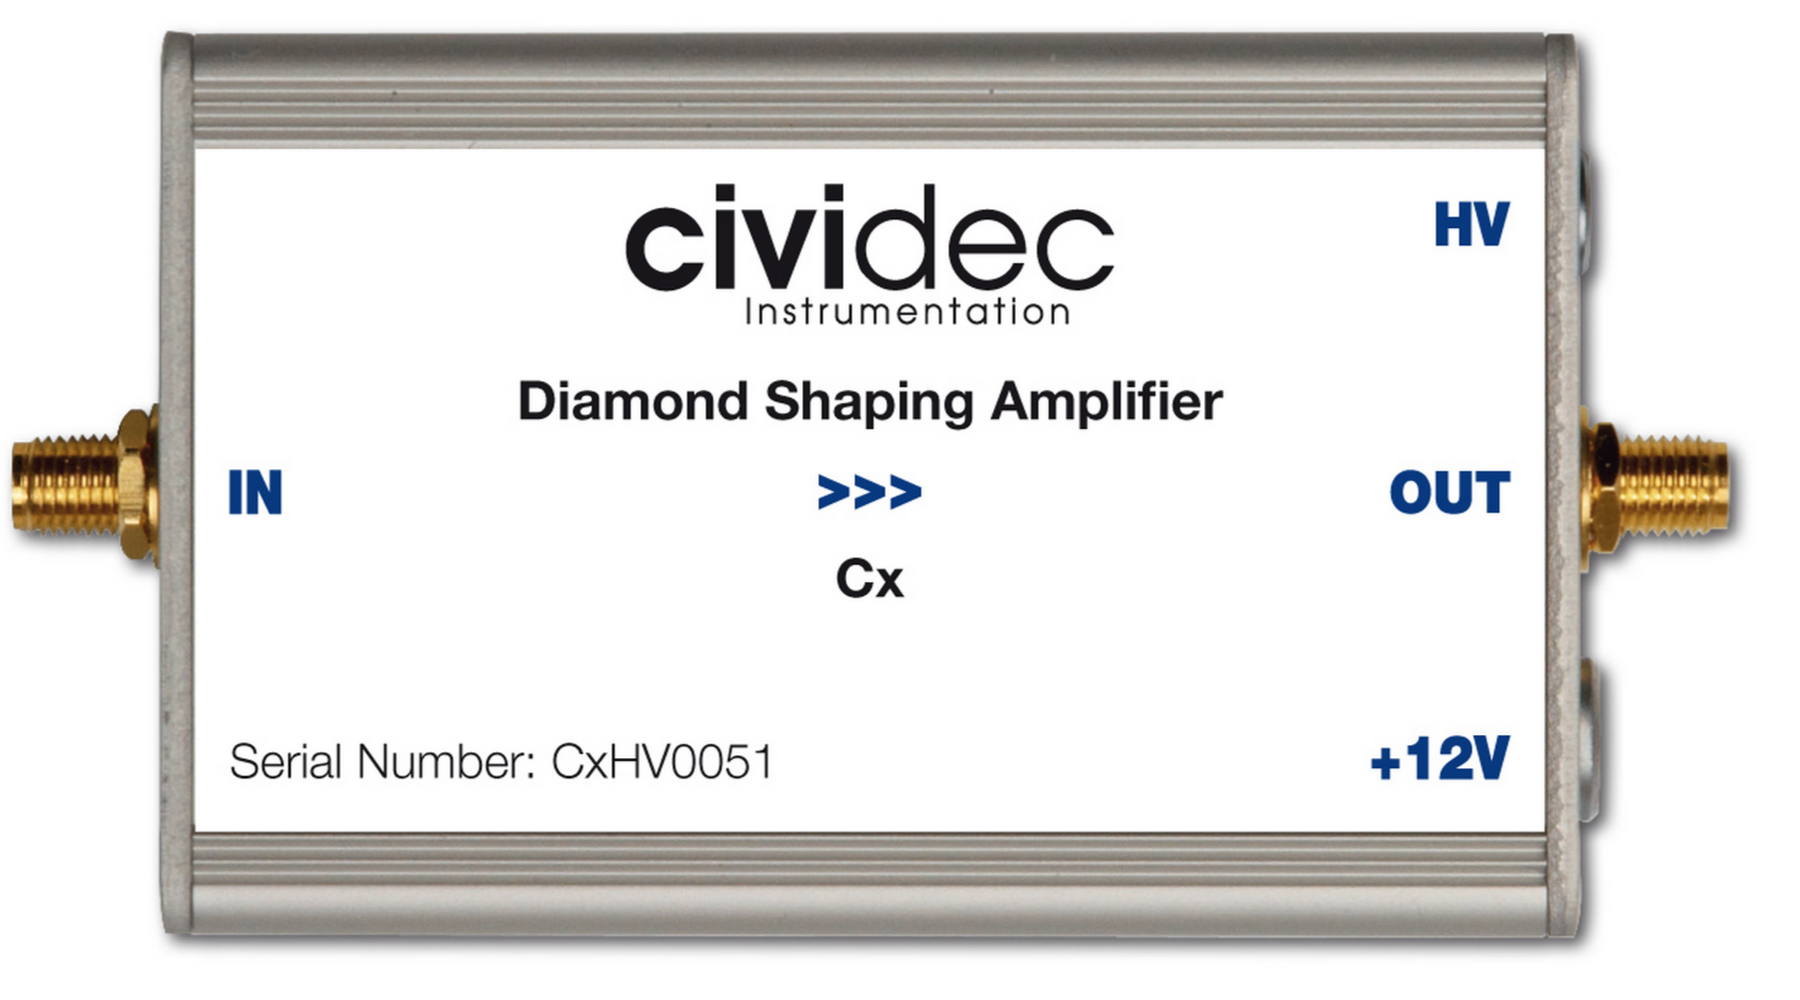
\includegraphics[width=0.45\textwidth]{pics/setup/Cx} \label{fig:ampcx}} &
\subfloat[C2 fast charge preamplifier]{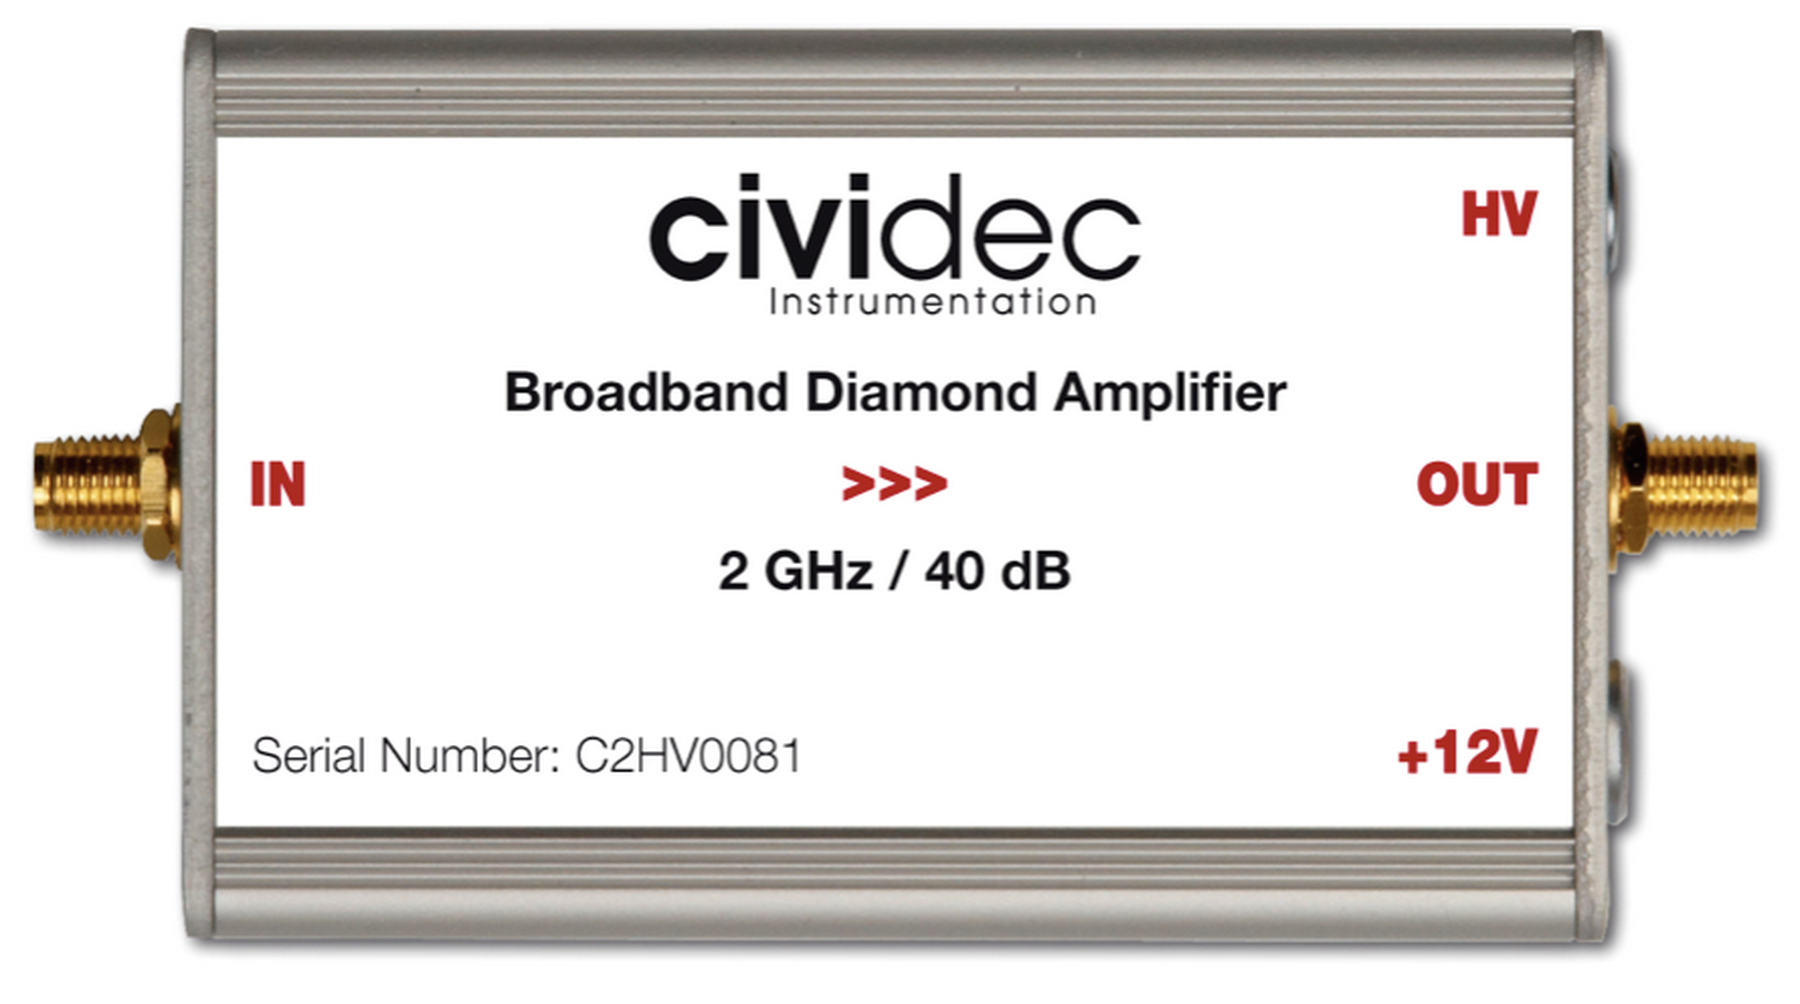
\includegraphics[width=0.45\textwidth]{pics/setup/C2}  \label{fig:ampc2}}
\end{tabular}
\caption{Amplifiers used for the charge and current measurements}
\end{figure}


\subsubsection{Calibration}
The amplifiers were calibrated before use to determine their gain. Both were calibrated using a square signal generator with a known amplitude step of $U_{in}=(252\pm5)$~mV. A 2~GHz oscilloscope with a 10~GS/s sampling was used to carry out these measurements. 

In the case of the Cx charge sensitive amplifier, the signal was routed through a capacitor with a calibration capacitance $C_{cal}=(0.717\pm0.014)$~pF and then to the input of the amplifier. The pulse area behind the capacitor was $a_{cal}=5.0\pm0.5)$~pVs and the signal amplitude on the output was $U_{amp}=(1.95\pm0.05)$~V. The input voltage step combined with the calibration capacitance yields a calibration charge $Q_{cal}=C_{cal}\cdot U_{in}=(181\pm5)$~fC. The gain of the Cx amplifier is therefore $A^{Q}_{Cx}=\frac{U_{Cx}{Q_{cal} }}=(9.3\pm0.4)$~mV/fC or  $A^{a}_{Cx}=\frac{U_{Cx}}{a_{cal} }=(390\pm40)$~mV/pVs. The area-based amplification factor has a higher uncertainty ($\sim10~\%$) than the amplitude-based factor ($\sim4~\%$) due to the measurement limitations of the oscilloscope. Nevertheless, it can be used as an estimate for the integrated charge of a current pulse.

To calibrate the C2 current amplifier, only the amplitude gain had to be measured. The input signal amplitude had to be such that it kept the output amplitude within the amplifier's linear range, that is $\pm1$~V. The signal from the generator was therefore routed through a 36~dB attenuator to decrease its amplitude to $U_{inAtt}=(3.95\pm0.05)$~mV. The output of the amplifier was $U_{amp}=(860\pm5)$~mV. This yields the amplification gain equal to $A_{C2}=\frac{U_{inAtt}}{U_{C2}} =(217\pm3)$.





\subsection{Diamond samples}
\label{sec:diamsam}
The diamond detector business is a niche market, with only a handful of producers existing worldwide. Detector-grade diamonds are very difficult to produce, mostly because it is very difficult to ensure a high enough purity of the lattice. It takes companies years of trials to produce high enough quality product. Since the target market are almost exclusively particle physics research institutes, the companies work closely with them to make sure the product is up to par with the requirements. All sensor samples used to carry out these studies were bought at Element Six (E6). They all have the same dimensions, which have become a kind of standard. sCVD diamonds with dimensions $4.7\times4.7$~mm$^2$ are already sufficiently large for most of the beam monitoring applications and still affordable; the price for sCVD diamonds grows exponentially with the area. There is also an ongoing race among the producers to produce larger and larger diamonds while maintaining the price tag. For instance, a rather young player in this field, IIa from Singapore, has produced high-quality samples with larger dimensions and the diamond detector community is currently involved in extensive tests of their products. One of the samples with dimensions of $5.6\times5.3$~mm$^2$ was also sent to the PH-ADE-ID group at CERN to be characterised. The target thickness for all the samples is 500~$\upmu$m. Diamonds this thick yield a high enough signal-to-noise ratio for MIPs to be measured by the electronics.
\begin{figure}
\centering
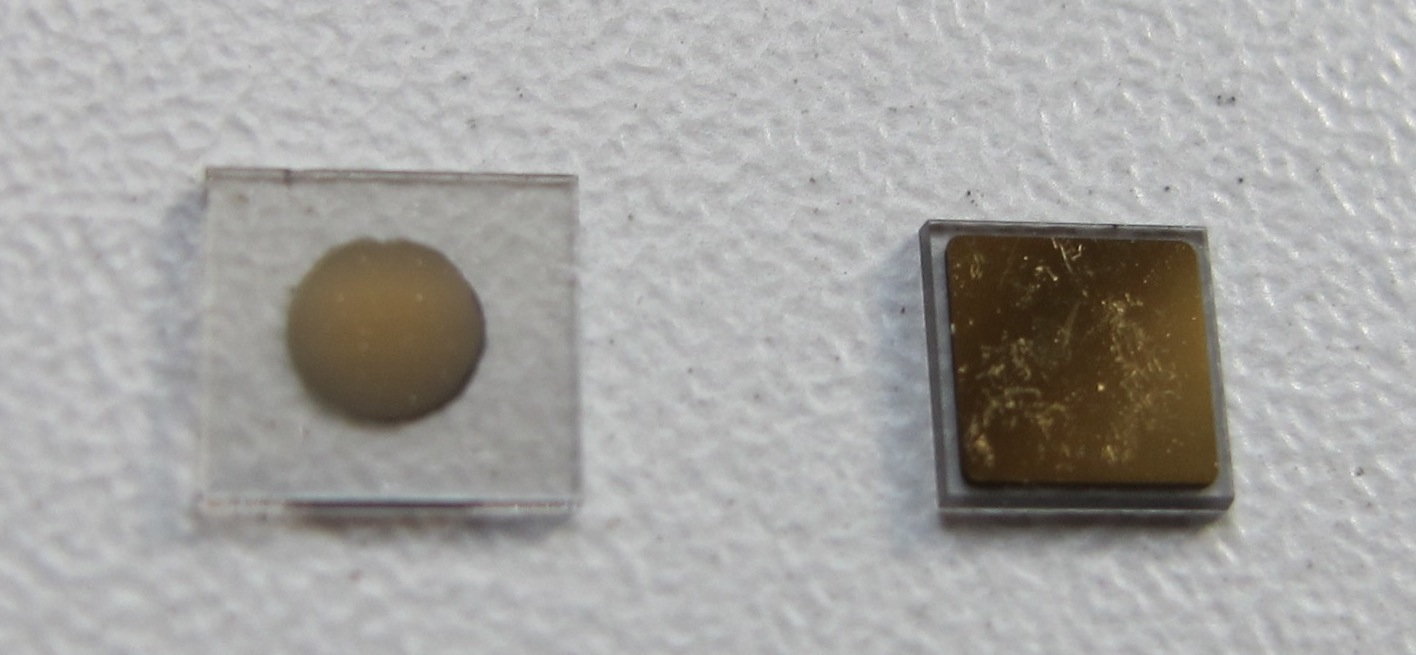
\includegraphics[width=0.8\textwidth]{pics/setup/diamond4}
\caption{Two scCVD diamond samples: A IIa 1scdhq (left) and an E6 S37 (right)}
\label{fig:diams}
\end{figure}
Table~\ref{tab:diamsamp} shows all the samples used for this study. Two of them were later irradiated with 300~MeV pions and then compared to the pre-irradiated state. Irradiation doses for damaging the material need to be high -- above $10^{12}$~particles per cm$^2$ to be able to observe change in the sensor's behaviour. 

\begin{footnotesize}
\begin{center}
\captionof{table}{Diamond sensor samples used}
\begin{tabular}{   l  c  c  c  c c }
\hline
Name & Type &Producer & Dimensions (x, y) [mm$^2$] & Thickness [$\upmu$m] & Irradiatied \\
\hline
S37 & sCVD & E6 & $4.7\times4.7$ & 548 & no \\
S50 & sCVD & E6 & $4.7\times4.7$ & 537 & no \\
S52 & sCVD & E6 & $4.7\times4.7$ & 515 & $1\times10^{14}~p/cm^{-2}$ \\
S79 & sCVD & E6 & $4.7\times4.7$ & 529 & $3.63\times10^{14}~p/cm^{-2}$ \\
ELSC & sCVD & E6 & $4.7\times4.7$ & 491 & no \\
1scdhq & sCVD & IIa & $5.6\times5.3$ & 460 & no \\
\hline
\end{tabular}
\label{tab:diamsamp}
\end{center}
\end{footnotesize}

The diamond samples have quoted impurity densities of $\leq2\times10^{14}$~cm$^{-3}$ and nitrogen incorporation of $\leq1$~ppb. The electrodes were added by various companies and institutes. For instance, S52 was metallised by DDL while the Physics Department of the University of Firenze, Italy metallised the S79. There are also several techniques for producing the electrodes. The DDL contacts consist of three layers: DLC (diamond-like carbon)/Pt/Au with 4/10/200 nm thicknesses, respectively. The metallisation for S79, on the other hand is made up of Cr/Au with a total thickness of $\sim$400~nm. The area coverage also differs from sample to sample. Diamonds must not be metallised until the very edge as the proximity of contacts with a high potential can lead to sparking. However, since only the areas not covered by the metallisation are sensitive, this effectively reduces the sensitive area of the sensors. In the diamonds used here the effective area was anywhere from 9~mm$^2$ to 18~mm$^2$. Leakage current through the bulk was below 1~ns, but increased for the irradiated samples. The capacitance was of the order of (2.0$\pm$0.3)~pF.


\subsection{Readout devices}
\label{sec:readoutdev}
Electrical signals in diamond detectors are in the GHz frequency range. To preserve this information, the readout device has to have a high bandwidth limit. For instance, a 250~MHz limit is enough for the spectroscopic measurements with the Cx charge amplifier, but might be insufficient for the current measurements with the C2 amplifier. Two devices were used take data shown in this chapter. The first choice was a 2~GHz LeCroy WaveRunner 204MXi-A. This specific model has a high enough limit for the fast current preamplifier signals. It offers a versatile solution for analogue signal readout -- it is fast to set up and reliable. It is very convenient for use in lab tests and for experiments where small amounts of data are taken and where speed is not crucial. However, its slow acquisition speed turned out to be a bottleneck in the test beam experiment. Its initial 100~Hz readout rate decreased to a mere 20~Hz within 20 minutes, because every single trigger was saved as a separate file and the Windows operating system was not capable of handling 10000+ files in a single directory easily. This is why it was exchanged with a DRS4, an analogue readout device developed by PSI, Switzerland. This compact device is capable of recording up to four waveforms at a time at a steady rate of up to 500~Hz. Its 700~MHz bandwidth limitation was sufficient for the signal from the charge amplifier.



\subsection{Setup for the efficiency study using $\upbeta$ particles}
The efficiency study of the diamond sensors was carried out at CERN in a test beam facility called the North Hall. There a straight high-energy particle beam of 120~GeV pions (marked $\uppi$) was provided to the users to calibrate their detectors. The size of the beam was approximately $\sigma=10$~mm and the particle rate was of the order of $10^4~\uppi$~cm$^{-2}$~s$^{-1}$. A diamond sensor embedded in a PCB carrier was placed in the beam spot perpendicular to the beam. It was connected via an SMA connector directly to a charge amplifier (described below). The amplified signal was read out using a LeCroy oscilloscope and a DRS4 analogue readout system (both described below). A computer was used as a controller and data storage for the readout device. A separate system was used as a reference detector. The so-called \emph{beam telescope} is a device used to cross-check the measurements of the devices under test (DUTs) and to carry out spatially resolved studies on the DUTs. It consists of several pixellated sensor planes placed in series, which can track a particle's trajectory with a precision of a few microns. The sensor planes are positioned in front of the DUT and behind it. Then the beam telescope acts as a trigger system -- it triggers the readout of both the telescope data and DUT data when both the planes in front and behind the DUT recorded a hit by the impinging particle. A particle detected by all the planes within the DUT window and the DUT itself counts towards its efficiency whereas a hit missed by the DUT counts against it. To discard the hits missing the DUT, a region of interest (ROI) can be chosen in the beam telescope planes.


\subsection{$\upalpha$-TCT setup}
Room-temperature TCT measurements were carried out in the lab. The setup consisted of a diamond sensor embedded in a PCB carrier, a current amplifier and an oscilloscope. To measure $\upalpha$ particles, their energy loss during their trajectory had to be minimised. Therefore the diamond was placed inside a vacuum chamber. The chamber was a steel tube with a diameter of 5~cm. On one side it was connected to a vacuum pump via an steel pipe. A feedthrough with an SMA connector was placed on the other side. A C2 current amplifier was connected directly onto the feedthrough. The amplified output was connected to the oscilloscope via an SMA cable. An $^{241}$Am source with a diameter of 2~cm and a height of 0.5~cm was placed onto the sensor carrier (figure~\ref{fig:carrier}) and fixed in place using kapton tape (figure~\ref{fig:carsrc}). Then the carrier was inserted in the chamber and fixed in place using an air-tight clamp. The pump was then switched on. It was capable of providing the inside pressure as low as $10^{-4}$~mbar after approximately one hour of operation, but measurements could take place even after five minutes of evacuation, at around $10^{-3}$~mbar. The most important thing to bear in mind was to switch the bias voltage of the sensor OFF during the process of evacuation, because the air becomes more conductive at the pressure of the order of $10^{-1}$~mbar. A failure to switch off the bias voltage would cause a spark between the signal and ground line, destroying the amplifier. Yes, this did happen in the course of carrying out these measurements.

\begin{figure}[!t]
%\centering
\begin{tabular}{cccc}
\subfloat[PCB carrier with an embedded diamond sample]{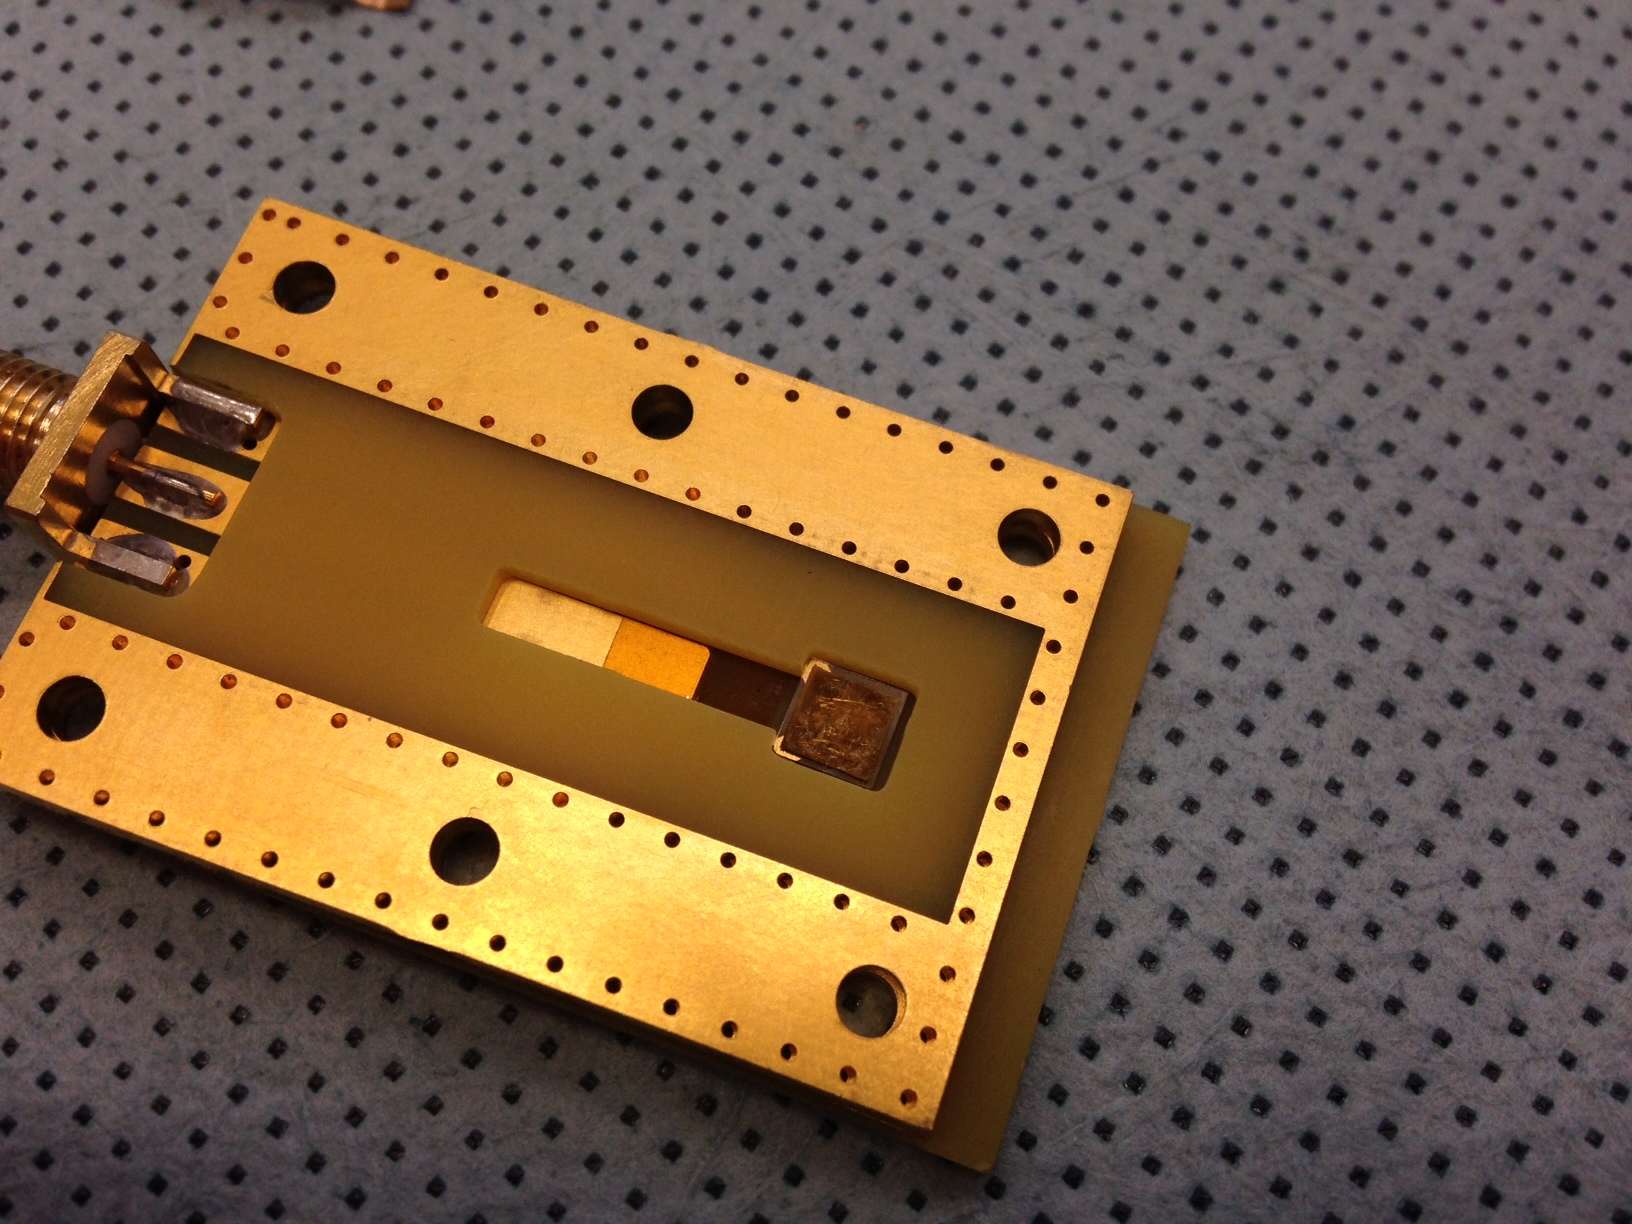
\includegraphics[width=0.45\textwidth]{pics/setup/carrier2} \label{fig:carrier}} &
\subfloat[Radioactive source over the carrier]{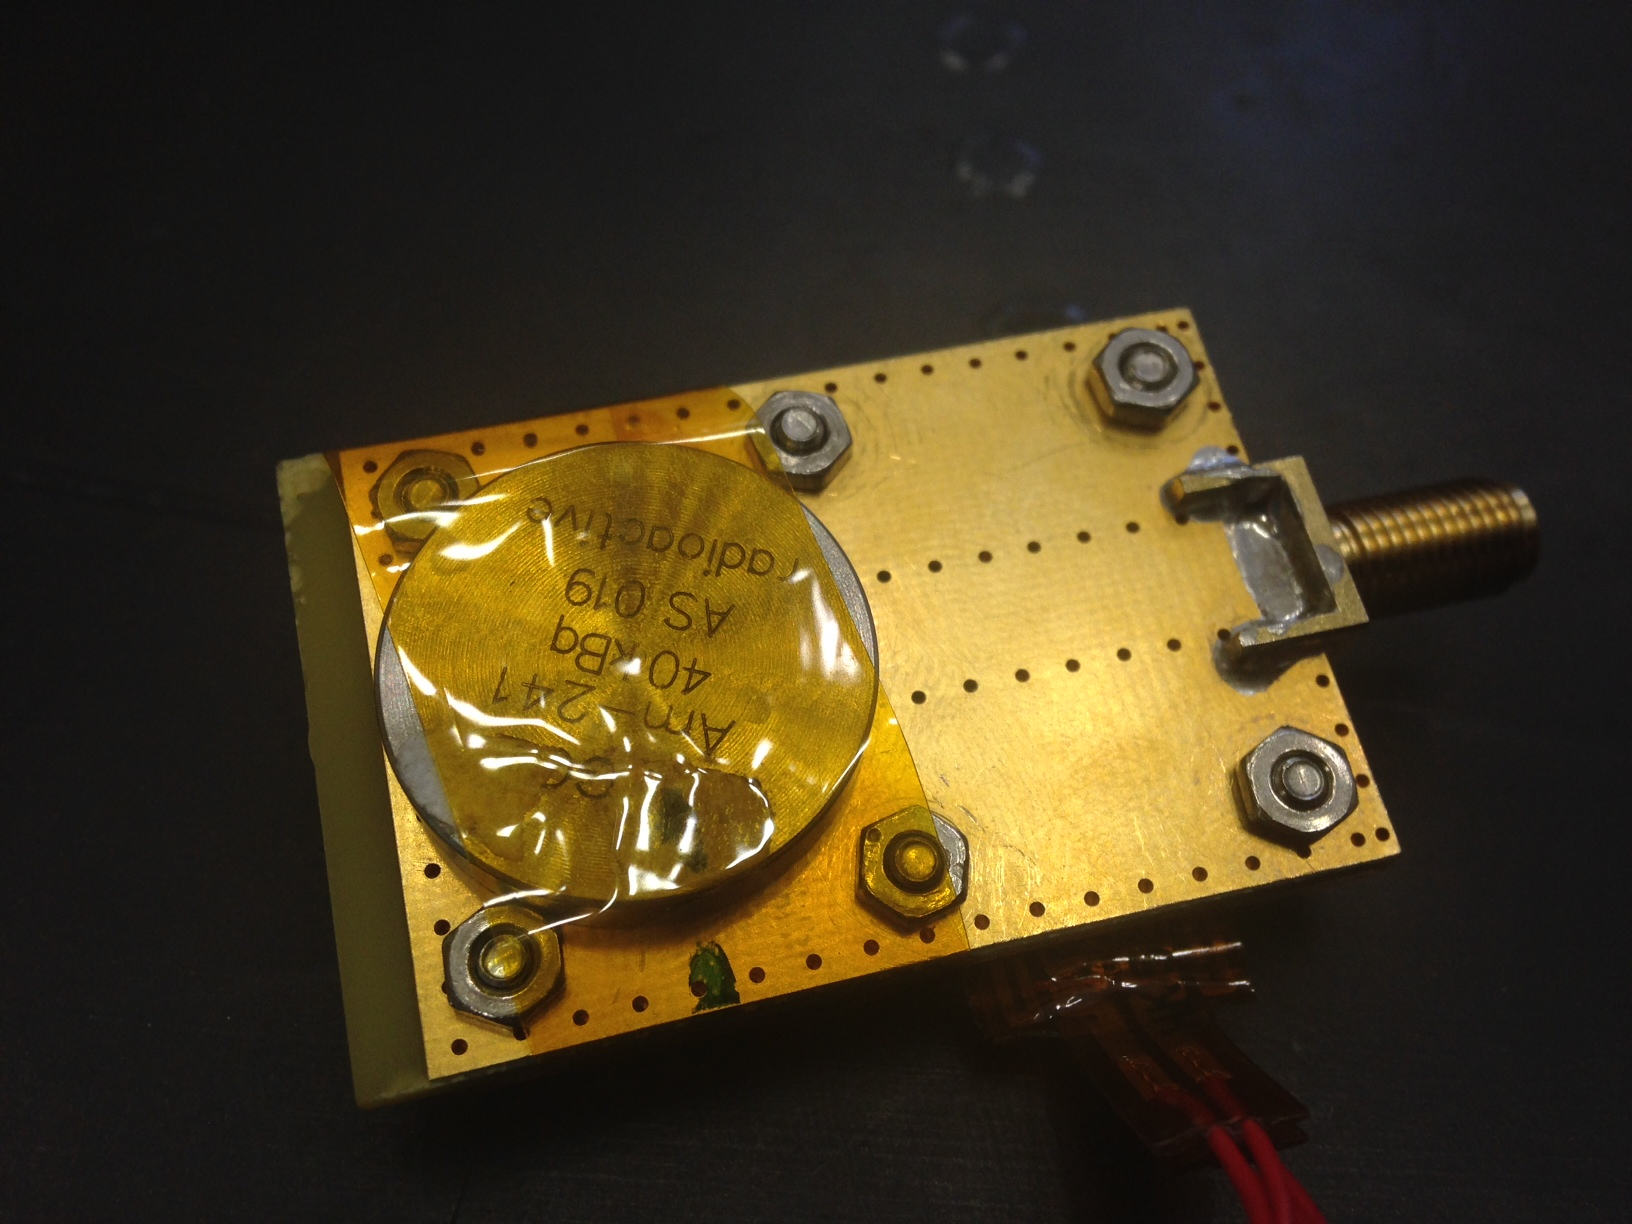
\includegraphics[width=0.45\textwidth]{pics/setup/carriersource2}  \label{fig:carsrc}}
\end{tabular}
\caption{Positioning of the $\upalpha$-source on top of the sensor carrier}
\end{figure}


\subsection{Cryogenic $\upalpha$-TCT setup}
\label{sec:cryosetup}
The experiment at cryogenic temperatures was carried out in the cryolab at CERN. The room-temperature TCT setup had to be modified to allow for measurements at temperatures as low as 2~K. It consisted of three parts: 1) a cryostat --  a thermally insulated cylinder capable of containing liquid helium, 2) an inlet -- an air-tight mechanical tube with valves and feedthroughs at the top that is lowered in the liquid helium and 3) the diamond sample, a temperature sensor, a heater and cables leading to the feedthroughs.

When the diamond sample was placed in the PCB carrier and the $^{241}$Am source was in place, the inlet was sealed and lowered in the empty cryostat. Then the inside volume of the inlet was evacuated to down to $10^{-5}$~mbar while the liquid helium was flowing into the cryostat. To improve the thermal contact between the diamond and the outside of the inlet, a small amount of helium gas was added inside the evacuated inlet, setting the vacuum to around $10^{-3}$~mbar. This value changed with time, because the gas condensed on the walls of the inlet, reducing the number of floating particles. For this reason the helium gas had to be added from time. This caused a significant undershoot of the sample temperature, which had to be corrected for with the heater. Also, the added gas deteriorated the vacuum inside the inlet. It was very important to monitor the pressure so as not to let it rise above $10^{-2}$~mbar. The air at this pressure is significantly more conductive and could cause a short circuit between the two diamond plates or in the SMA connectors, destroying the amplifier. Actually, it once did. Furthermore, at approximately 60~K the helium gas had to be evacuated from the inlet to avoid a potential explosion due to the expansion of the gas with temperature. Anyway, when the sample was cooled to the minimum temperature achievable by use of liquid helium without over-pressurising it (4.2~K), the measurements started. After every temperature data point, the current through the heater placed in the PCB next to the diamond sample was increased, warming up the sample. The initial temperature time constant of the order of tenths of seconds at low temperatures increased with temperature and even more so when helium was evacuated from the inlet at 60-~K, removing the thermal bridge between the wall of the inlet and the diamond sample. At RT, the time constant was already of the order of minutes.







%TCT, testbeam DISCUSSED IN CHAPTER 2!!!!!



% ---------------------------------------------------------------------------------------------------------------
%\clearpage
\section{Particle and photon pulses and spectra}
\label{sec:pulsespectra}
% ---------------------------------------------------------------------------------------------------------------
In previous chapter the ionisation profiles for different types of radiation were discussed. It is known that $\upbeta$ particles and $\upgamma$ radiation both create a triangular pulse whereas $\upalpha$ particles create a rectangular one. However, their amplitude, width and rise/fall time depend heavily on the type of interaction with the diamond, the purity of the diamond and the bandwidth of the amplifier and the oscilloscope. This section shows the signal pulses of $\upalpha, \upbeta$ and $\upgamma$ radiation with their respective energy distributions for the case of a diamond detector. Then follows a discussion of effects of noise on these measurements. 

A CIVIDEC C2 current amplifier together with the LeCroy oscilloscope (both with a bandwidth limit of 2~GHz) was used to record the pulse shapes whereas the Cx charge amplifier was used for area distribution measurement. A 2~GHz bandwidth limit defines the minimum rising time equal to $t_{r}\simeq\frac{0.34}{BW}=\frac{0.34}{2\times10^9}=170$~ps, therefore the system is capable of measuring pulses with a minimum FWHM$\simeq170~ps$. This already makes impossible to measure the initial peak in $\upalpha$ response due to the two flavours of charge carriers travelling. If the flavour travelling through the bulk takes t$_{t1}\sim~$6~ns to get to the electrode on the other side (d$_1\sim500~\upmu m$), the other with a shorter path to the closer electrode -- max. d$_2\sim10~\upmu$m -- already recombines in t$_{t2}\sim \frac{d_2}{d_1}t_{t1}=120$~ps. This is too fast for the C2 amplifier or the oscilloscope to be able to observe.

Figure~\ref{fig:pulsesaby} shows a set of pulses and an averaged pulse for $\upalpha, \upbeta$ and $\upgamma$ radiation as measured by the non-irradiated sCVD diamond S37. $\upalpha$ particles always produce the same signal pulse, with a high noise RMS. The averaging suppresses the noise while still retaining most the information. It does, however, smear the rising and falling edge, increasing the rise time. The t$_{r}$ is now of the order of 0.5~ns. Both $\upbeta$ and $\upgamma$ pulses look similar - triangular and with a wide range of amplitudes. Here the pulse count is low, so the really high pulses were not recorded, because they are very rare. A trigger set very high would be needed to "catch" them with the oscilloscope.

\begin{figure}[!t]
%\centering
\begin{tabular}{rrr}
%\subfloat[$\upalpha$ pulses]{\includegraphics[width=0.27\textwidth]{} \label{fig:alpha1}} &
%\subfloat[$\upbeta$ pulses]{\includegraphics[width=0.27\textwidth]{}  \label{fig:beta1}} &
%\subfloat[$\upgamma$ pulses]{\includegraphics[width=0.27\textwidth]{}  \label{fig:gamma1}}
\end{tabular}
\caption{PLACEHOLDER Current pulses for three types of radiation}
\label{fig:pulsesaby}
\end{figure}

%---------------------------------------------------------------------------------------------------------------
%%\clearpage
\subsection{Noise limitations}
\label{sec:noiselimit}
%---------------------------------------------------------------------------------------------------------------
%TO DO: Take 8 runs with the 2GHz oscilloscope while increasing the noise. 
%TO DO: leakage current, irradiated.
Noise is a major limiting factor in particle detection. It defines the minimum measurable particle energy and the minimum measurement resolution. It is hence important to minimise the electric noise in the detector signal. The major noise contribution comes from poor shielding from external electromagnetic sources. These often cause so-called ringing, whereby the signal oscillates with a frequency defined by the external source. The ringing makes high-frequency measurements impossible. Another source of noise is the sensor itself. In the case of silicon, natural light increases the number of thermally excited free charge carriers, increasing the leakage current. This is not the case for diamond, which is with its high energy band gap insensitive to visible light. Nevertheless, any noise produced by the sensors is amplified by the signal amplifiers, which add an additional noise of the analogue electrical circuit to the amplified signal. Finally, the digitisers add the quantisation noise to the digitised signal. If the measurement range is significantly higher than the actual measured signal, the quantisation noise can be a significant contributor to the decrease of the overall measurement resolution.






% ---------------------------------------------------------------------------------------------------------------
%\clearpage
\section{Radiation limitations}
\label{sec:radlimit}
% ---------------------------------------------------------------------------------------------------------------
Exposure to ionising radiation degrades sensors. It introduces so-called charge traps by damaging the sensor material. The electrons and holes created by the impinging particle get trapped in these traps, decreasing the induced current on the electrodes. This yields a lower integrated charge in an irradiated sensor than that in a non-irradiated one. Charge collection efficiency is therefore correlated with the level of irradiation. In semiconductors, it follows an inverse exponential curve ?????

\subsection{Quantifying radiation damage in diamonds}
The last few decades have seen extensive efforts put into understanding and quantifying radiation damage in semiconductors. This varies with the type of radiation (particles or photons) and its energy. There are models existing that try to explain the impact of irradiation and to provide \emph{hardness factors} to compare the radiation damage between different particles. The standard way is to convert the damage into \emph{neutron equivalent}. Some models have been extensively verified with simulations and experimentally. In these experiments charge collection in sensors is measured before and after irradiation. This procedure is repeated several times, with a measurement point taken after every irradiation. When a set of measurements of charge collection is plotted against the radiation dose received by a specific particle at a specific , a damage factor $k_\lambda$ can be extracted. Damage factors across a range of energies and types of particles (photons) have to be measured to properly quantify the damage in the sensors. They are then compared against the simulations to verify that the experimental observations are in line with the theory.

Radiation damage in silicon, for instance, is well understood and explained. Silicon sensor is relatively cheap and widespread, which facilitated the irradiation experiments. Diamond, however, is an expensive material and the technology is relatively new as compared to silicon. Therefore not many institutes are carrying out diamond irradiation studies. To join the efforts, a collaboration called RD42 was formed. It gathers the experimental data from diamond irradiation studies. Unlike with silicon, the experimental results so far show no significant correlation with the NIEL (non-ionising energy loss) model~\cite{XXX}, which correlates detector efficiency with the \emph{number of lattice displacements}. Therefore an alternative model was proposed by Karlsruhe Institute of Technology~\cite{XXX}, correlating the diamond efficiency with \emph{displacements per atom} (DPA) in the bulk. Figure~\ref{fig:kitdpa} shows the DPA model for a range of energies of proton, pion and neutron irradiation in diamond. It has been normalised to damage in 24~GeV protons. According to the plot, a 300~MeV pion beam damages the diamond bulk twice as much as a 24~GeV proton beam.


\begin{figure}[!t]
\begin{center}
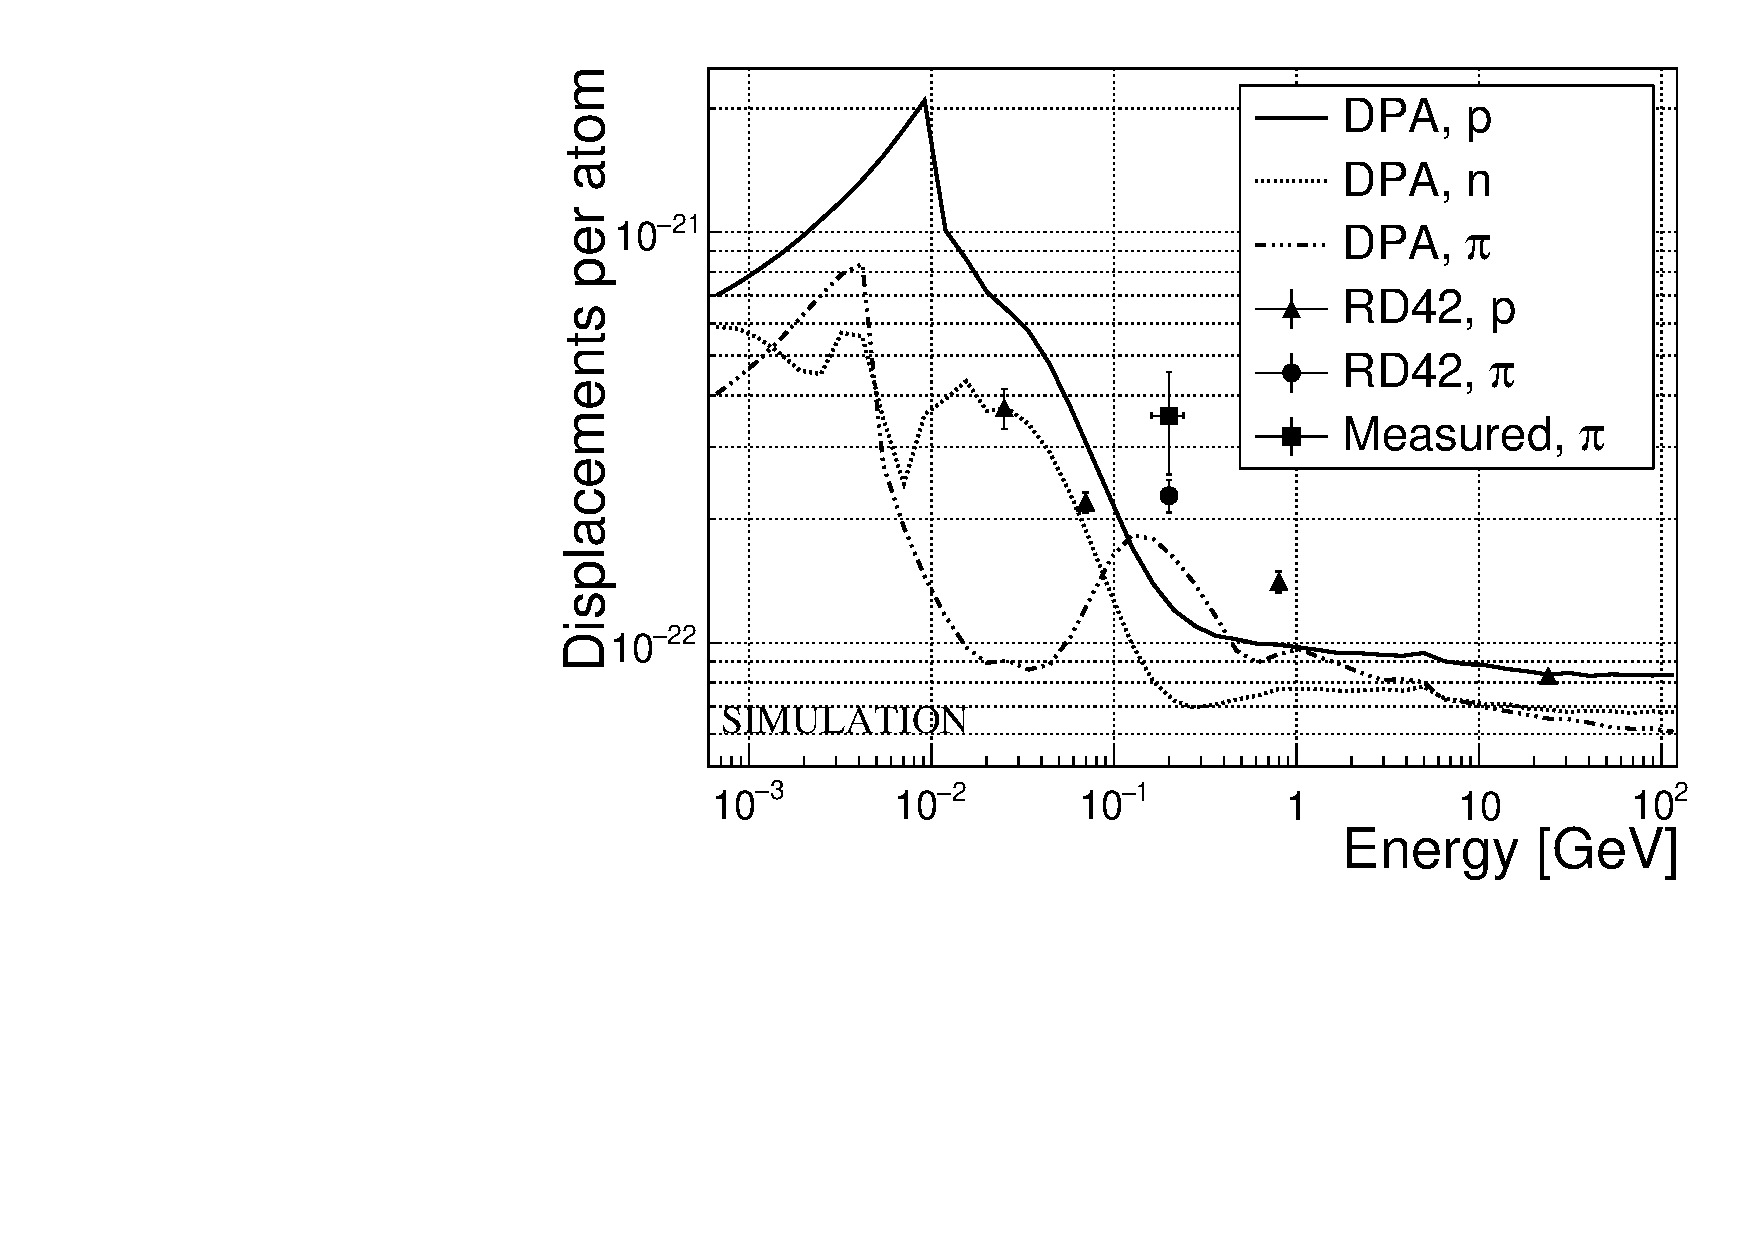
\includegraphics[width=0.6\textwidth]{scripts/plots/dpa1}
\caption{Diamond radiation damage - a model based on displacements per atom. Courtesy Karlsruhe Institute of Technology~\cite{}}
\label{fig:kitdpa}
\end{center}
\end{figure}



\subsubsection{Pion irradiation}
Paul Scherrer Institute (PSI) is the largest research institute for material sciences in Switzerland. Among other tasks they also carry out irradiation campaigns. They use a beam of    300~MeV/c pions $\pi$ (kinetic energy 191.31~MeV) with a flux of up to $1.5\times10^{14}~\pi$~cm$^{-2}$~day$^{-1}$. The machine has a 10~\% uncertainty on the beam energy. In addition, due to the uncertainty on the hardness factor, the equivalent fluences have an error of $\pm20~\%$. Looking at figure~\ref{fig:kitdpa}, $\pi_{300~MeV}$ sit on a steep section of the DPA function. After fitting a linear function to this part of the function (marked red), the error on the DPA due to the uncertainty on the beam energy amounts to 7~\%. Overall error on the fluence is therefore the root mean square of the uncertainty on the DPA and the uncertainty on the hardness factor: $\upsigma=21~\%$.

Two diamond samples, S52 and S79, were exposed to the pion beam in the 2014 PSI irradiation campaign; S52 to $(1\pm0.21)\times10^{14}~\pi$~cm$^{-2}$ and S79 to $(3.63\pm0.77\times10^{14}~\pi$~cm$^{-2}$. During the process, the golden electrodes got slightly activated, but the activation decayed in two weeks.

\subsubsection{Charge collection distance}
Three diamonds -- non-irradiated S37 and irradiated S52 and S79 -- were exposed to a 120~GeV test beam before and after irradiation to estimate the charge collection distance (CCD) and its decrease after irradiation. The samples were primed ("pumped") prior to data taking using a $^{90}$Sr radioactive source. Data were then taken at a range of bias voltages from 30~V to 500~V, yielding up to 1~V/$\upmu$m electrical field in the bulk. Every data point contained approximately $5\times10^4$ measured particles. The charge deposited by the particles was measured using a CIVIDEC Cx charge preamplifier. As expected, the integrated amplitude spectrum followed a landau distribution.
%, as seen in figure~\ref{fig:landausample}. 
Its most probable value (MPV) was used to calculate the most probable collected charge $Q_i$:
\begin{equation}
\label{eq:ccdcalc}
Q_i~[e] = Q_i~[fC] \cdot 6.241\times 10^{18} = \frac{MPV~[mV]}{A~[mV/fC]} \cdot 6.241\times 10^{18}
\end{equation} 
where A$=9.2$~mV/fC is the preamplifier gain factor. The CCD was then calculated using the average number of electron-hole pairs produced per micrometer in diamond $\delta_d = 36~$\emph{e-h}$~\mu m^{-1}$:
\begin{equation}
\label{eq:ccdcalc1}
CCD = \frac{Q_i}{\delta_d}
\end{equation} 

% sample landau distribution  
%\begin{figure}[!t]
%\begin{center}
%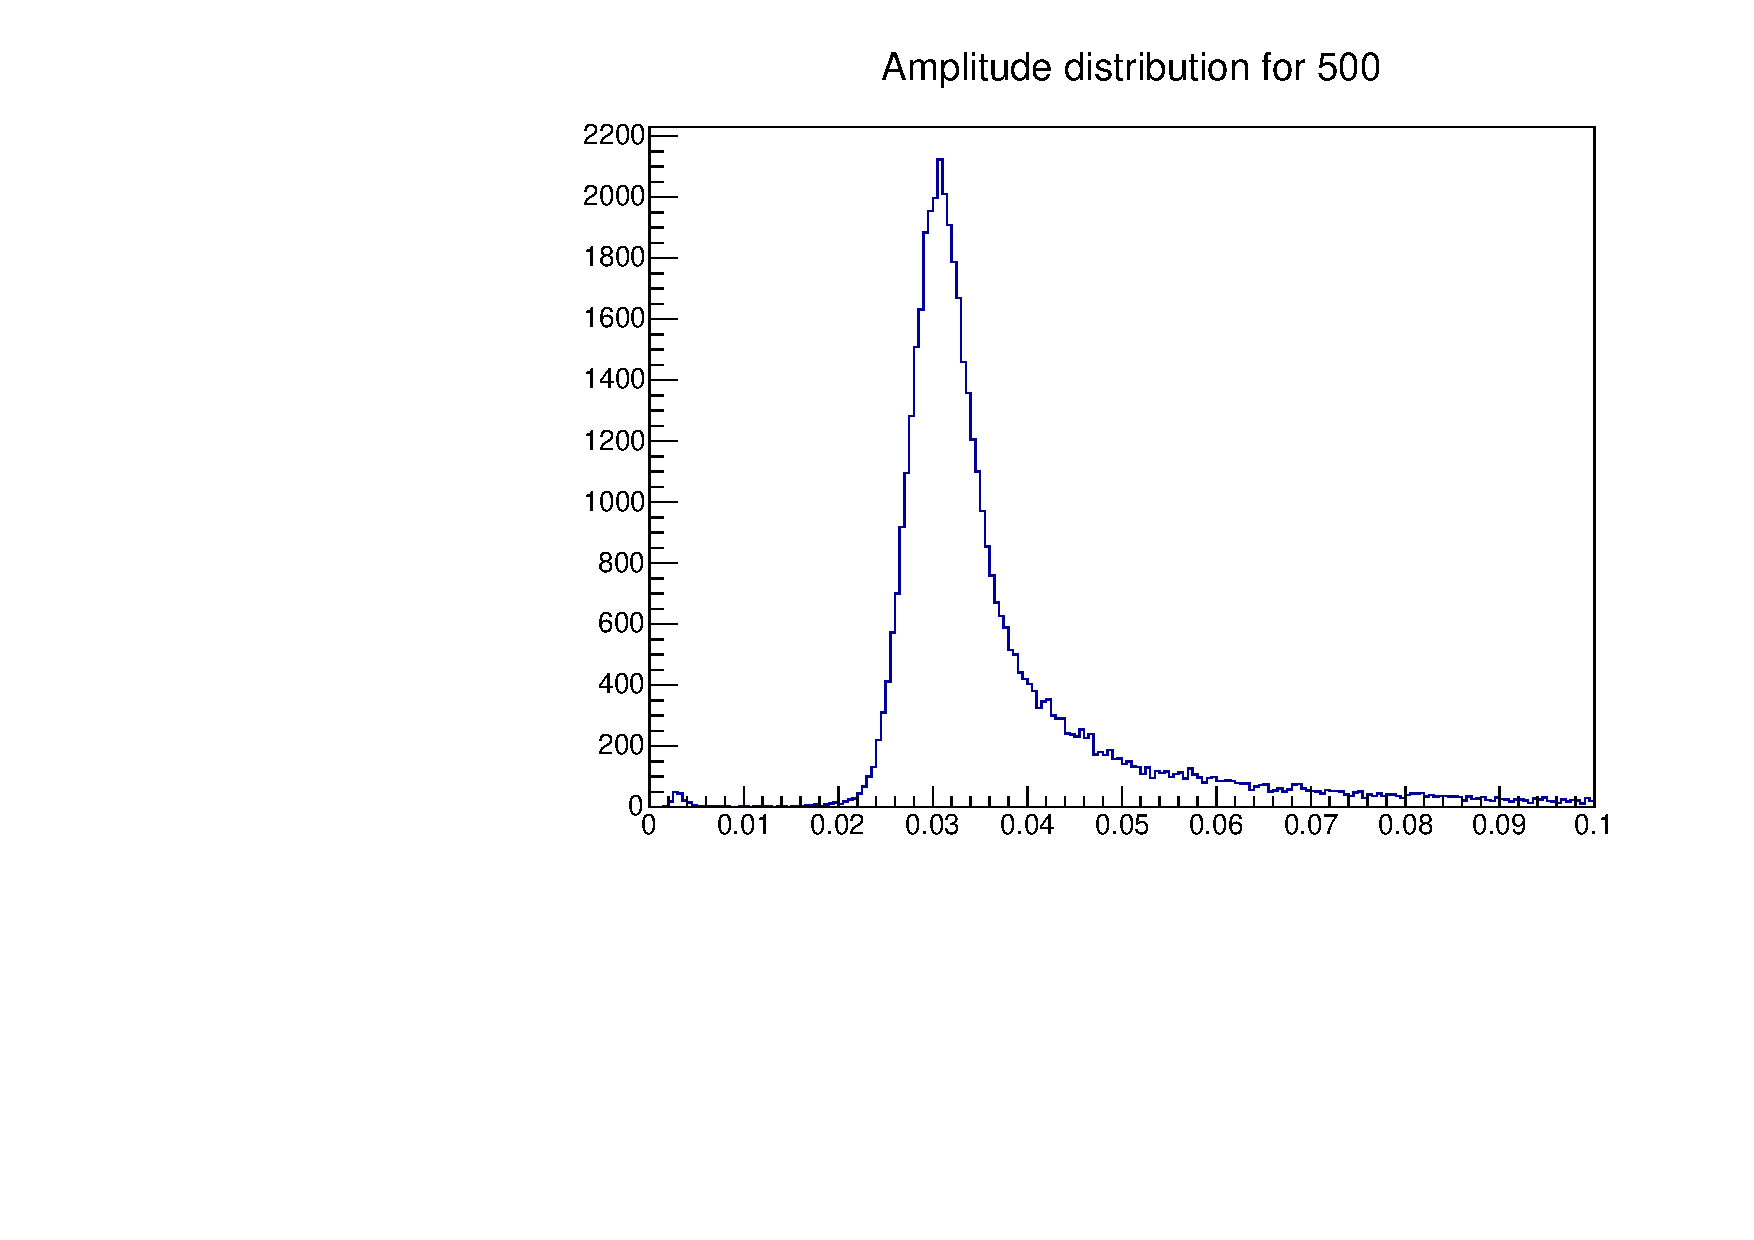
\includegraphics[width=0.6\textwidth]{scripts/pics/S37_500}
%\caption{An example of a landau distribution acquired by S37 at 500~V bias voltage PLACEHOLDER}
%\label{fig:landausample}
%\end{center}
%\end{figure}
The resulting CCD for the three measured samples at bias voltages ranging from 0.2--1.6~V~$\upmu$m$^{-1}$ is shown in figure~\ref{fig:ccd}. S37 exhibits full collection distance already at 0.4~V~$\upmu$m$^{-1}$ whereas the irradiated samples have a more gentle increase of CCD with increasing bias voltage. It is evident that at 1~V~$\upmu$m$^{-1}$  the maximum CCD has not been reached in the case of S79 and S52.

% CCD against HV 
\begin{figure}[!t]
%\centering
\begin{tabular}{cccc}
\subfloat[CCD for S37, S79 and S52]{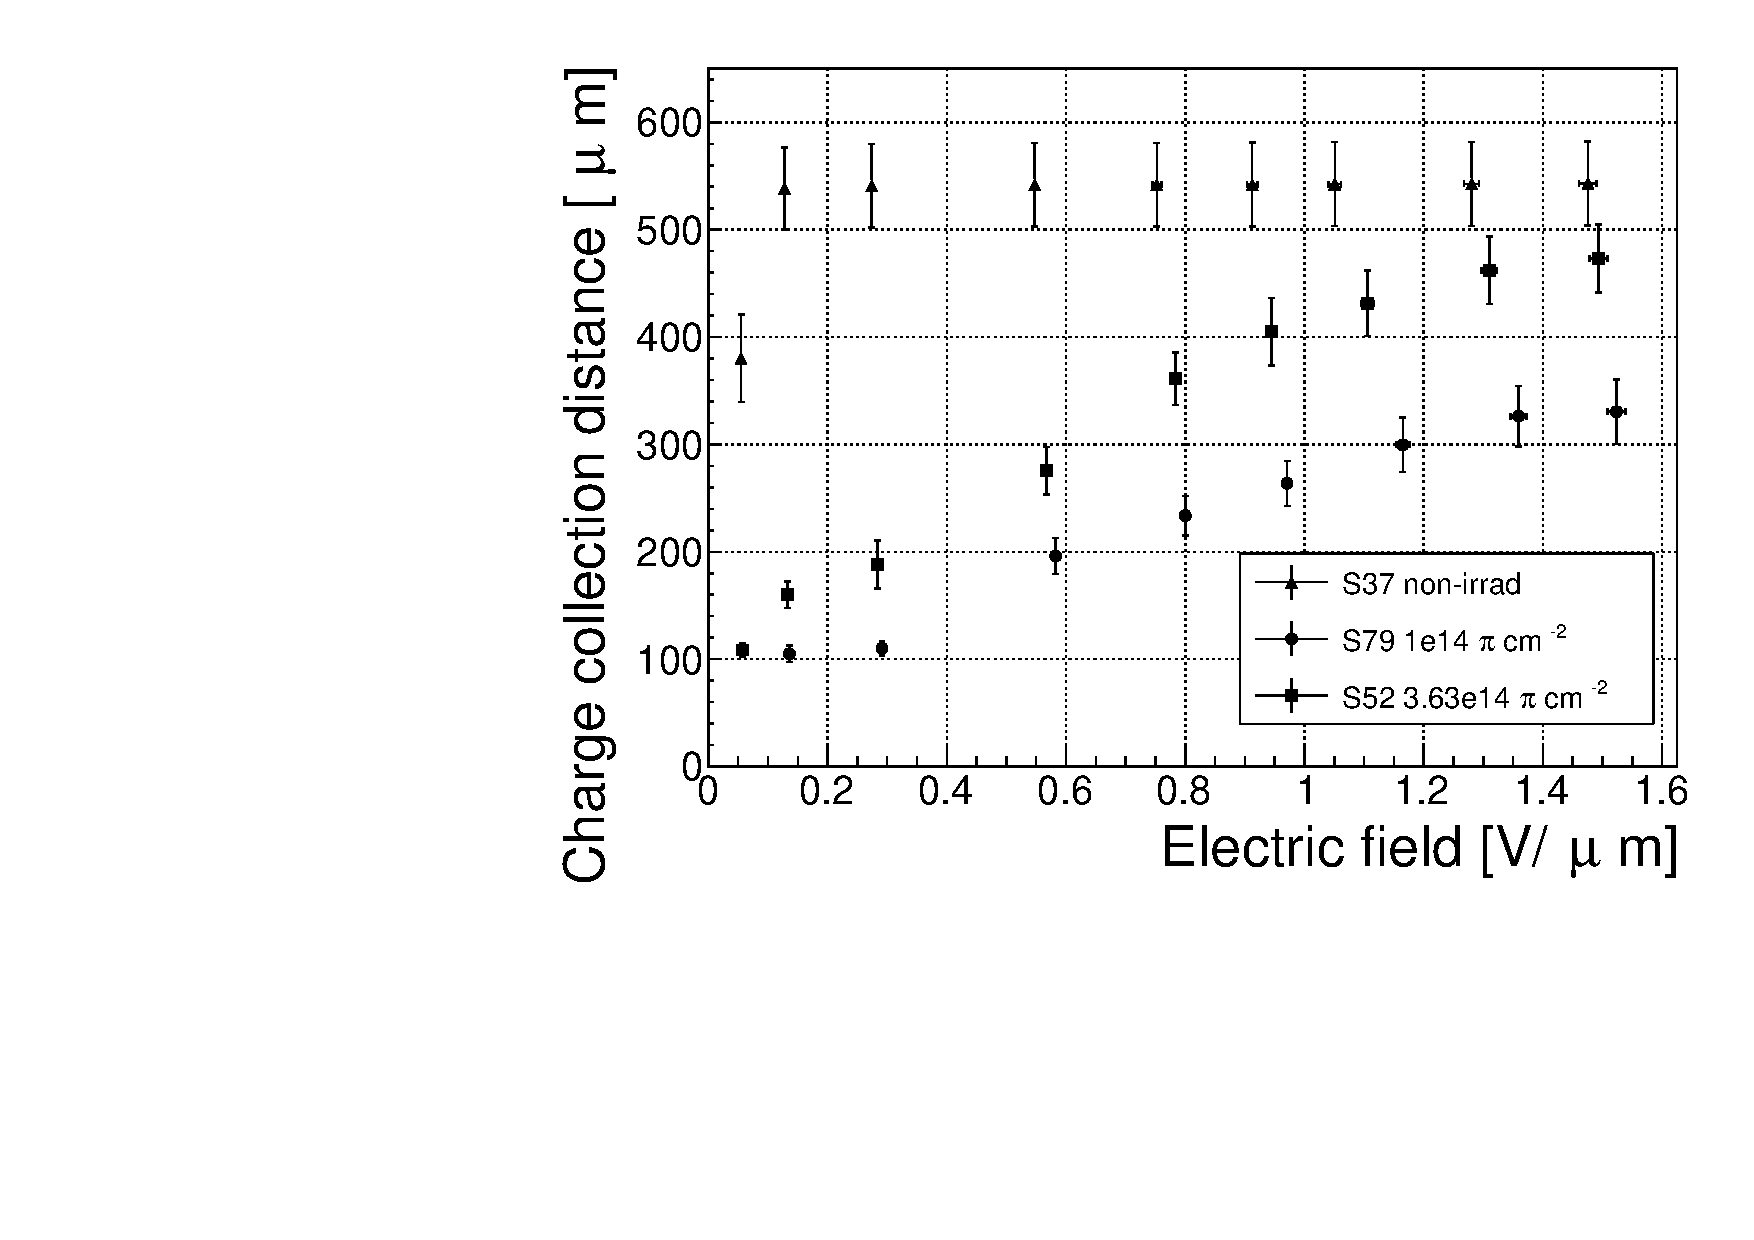
\includegraphics[width=0.45\textwidth]{scripts/plots/ccd} \label{fig:ccd}} &
\subfloat[Comparing the data points obtained in a test beam against the RD42 data]{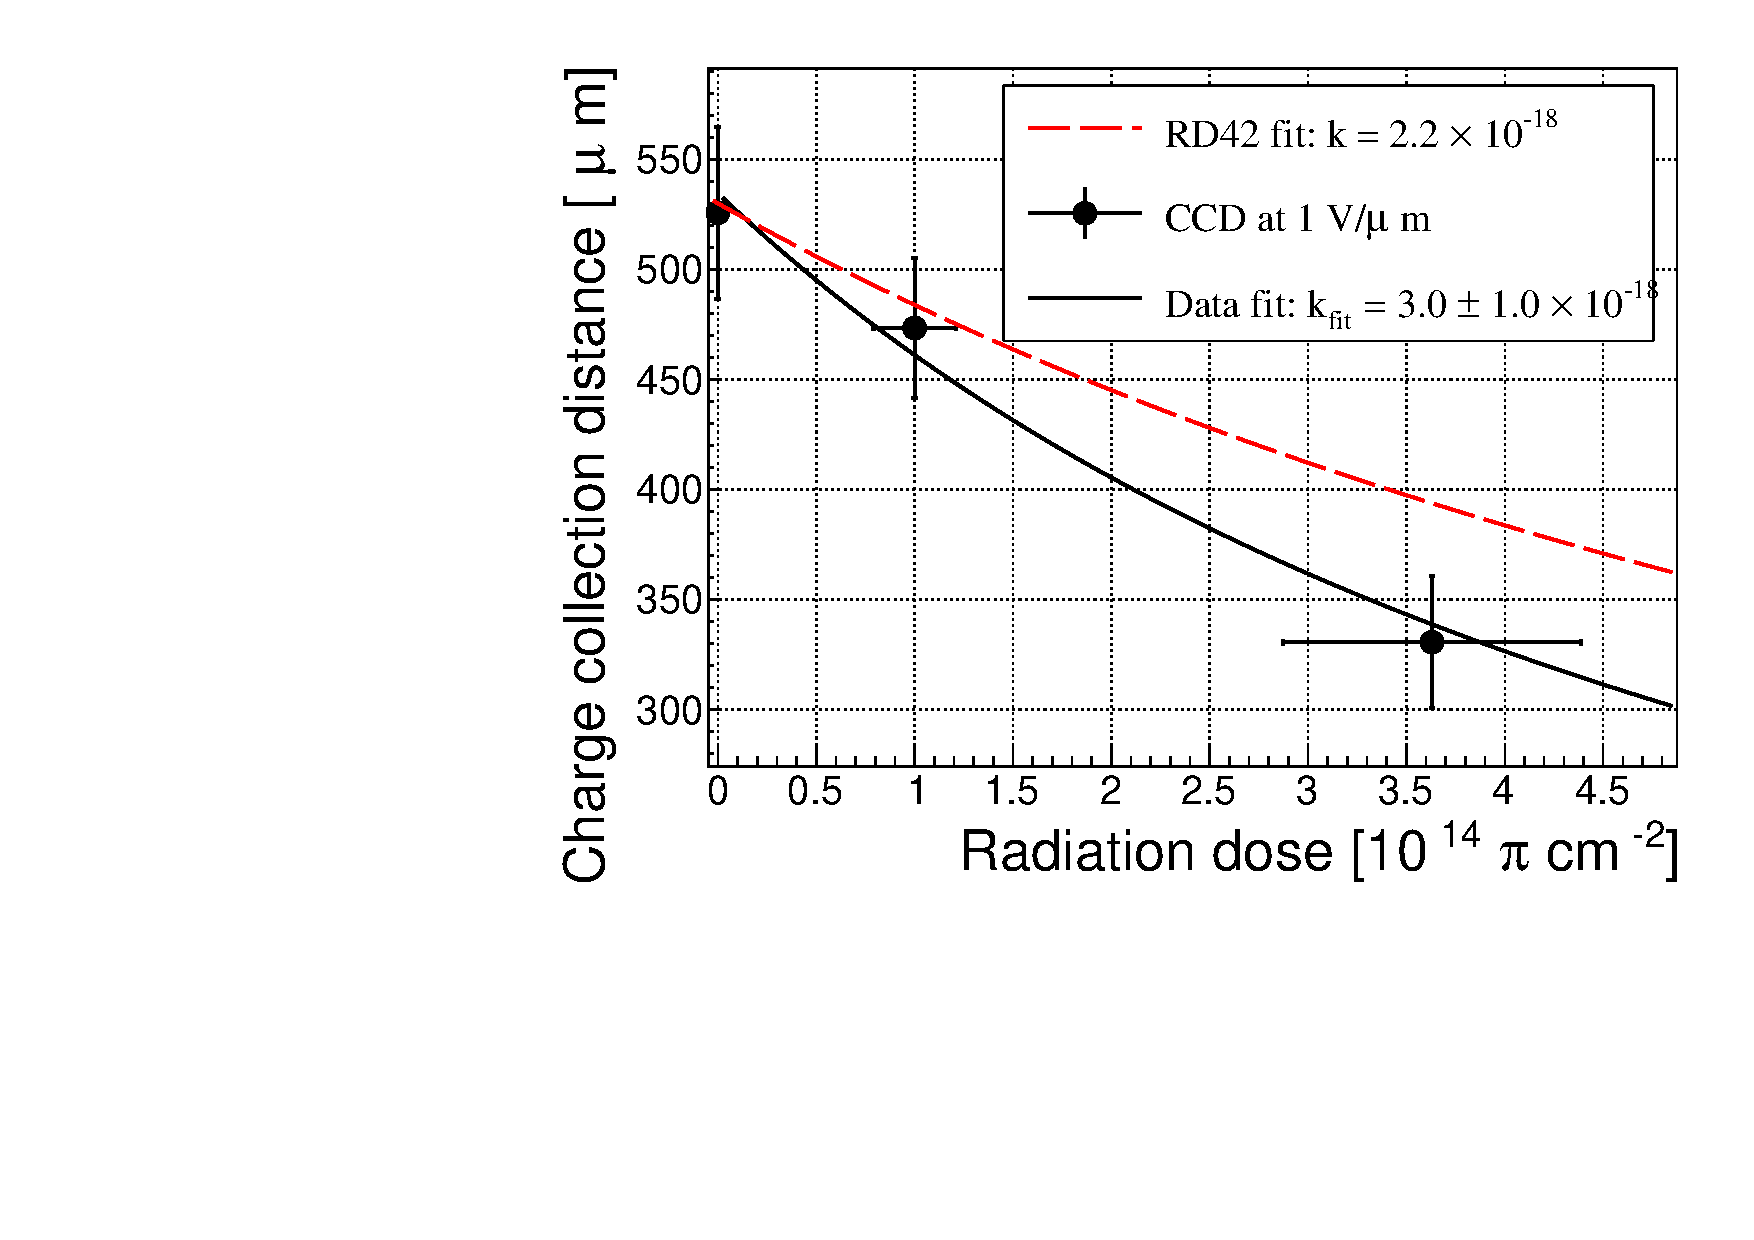
\includegraphics[width=0.45\textwidth]{scripts/plots/radfactor}  \label{fig:radfactor}}
\end{tabular}
\caption{The charge collection distance at 500~V bias voltage for the three diamond samples was compared to the RD42 data for pion irradiation. The data points are for about 5--15~\% lower than expected from the RD42 data.}
\end{figure}

\subsubsection{Irradiation damage factor}
The irradiation damage factor $k$ is a way to quantify irradiation damage of a specific particle at a specific energy. Via this factor different types of irradiation can be compared. It is obtained experimentally by measuring the CCD of a number of samples at various irradiation steps and fitting the function~\ref{eq:radfactor1} to the data. $\lambda$ is the measured CCD, $\lambda_0$ is the CCD of a non-irradiated sample and $\Phi$ the radiation dose.


\begin{equation}
\label{eq:radfactor}
\frac{1}{\lambda} = \frac{1}{\lambda_0}+k_{\Lambda}\cdot\Phi
\end{equation} 
\begin{equation}
\label{eq:radfactor1}
\lambda = \frac{\lambda_0}{k_{\Lambda} \lambda_0 \Phi + 1}
\end{equation} 

The data points with the maximum CCD obtained in the test beam measurements were plotted against radiation dose received (see figure~\ref{fig:radfactor}). Function~\ref{eq:radfactor1} was fitted to the data points and a damage factor $k_{\Lambda}=(3.2\pm1)\times10^{-18}~\upmu$m$^{-1}$~cm~$^{-2}$ was obtained. This value is higher than the damage factor obtained by RD42. A possible cause is that the irradiated samples did not yet have a full charge collection at 1.5~V~$\upmu$m$^{-1}$.




\subsection{Long-term measurement stability}
An important requirement for particle detectors is stable performance over long periods of time. For instance, the charge collection for a defined type and quantity of radiation must not change over time or has to change in a predicted way. Diamonds are arguably stable, as long as their environment and operating point does not change. The stability of diamond detectors depends on many external factors. The aim is to study the behaviour of diamond under controlled conditions, with the goal to understand its limitations. One of these limitations is for sure the received radiation dose. It might affect the long-term stability of the sensor during operation. 

The three diamond samples (S37, S79 and S52) were exposed to two different types of ionising radiation for a longer period to see if their behaviour changes over time. Two parameters were observed in particular: 1) charge collection of $\upbeta$ particles and 2) charge collection and ionisation profile of $\upalpha$ particles. The results showed in both cases that \emph{priming} plays an important role in diamond measurement stability. The $\upbeta$ particles have a healing effect on the diamond; MIP detection is therefore rather stable in the long run, despite the degradation due to irradiation. Alpha particles, on the other hand, deteriorate the measurement by introducing space charge into the sensor bulk. 

\subsubsection{$\upbeta$ measurements}
The samples were intentionally not primed before the measurements took place. The same initial conditions are usually found in HEP experiments. The measurement setup consisted of a diamond sample with the Cx spectroscopic amplifier, a silicon diode with a C6 amplifier for a trigger and a $^{90}$Sr source on top. A particle emitted by the source traversed the sensor bulk and hit the silicon diode, triggering the analogue signal readout. The source was left on the top for the course of the experiment. The measurements, however, took place at discrete times. For every data point, approximately $10^4$ triggers were recorded. The offline analysis of the recorded signal pulse amplitudes yielded a landau distribution for every data point. The resulting graph of charge collection over time showed that the charge collection efficiency improves over time. This is especially evident in the case of the two irradiated samples. S79 achieves close to full efficiency whereas S52 reaches about 75~\%. Both increases are significant. After some time the signal stabilises. As expected, the signal of the non-irradiated S37 did not change with time -- this pure sCVD diamond sample had the maximum collection efficiency from the start.

It should be noted that the $\sim$2.28~MeV electrons emitted by this source are not MIPs, because they sit far to the left on the Bethe-Bloch function and therefore deposit more charge in the bulk than the regular MIPs. Nevertheless, for the purpose of these measurements this energy was adequate since only the relative change in charge collection was of our interest.

To sum up, diamond is an adequate material for use in $\upbeta$ radiation detection. Even if damaged by radiation, it reaches equilibrium in the order of an hour and exhibits stable charge collection from then on. The efficiency decreases with received radiation dose, but the decrease can be accounted for if the damage factor and the rate energy of the particles are known. 

$\upgamma$ radiation has a similar impact on the diamond as the $\upbeta$. The impinging photons prime the diamond bulk, causing the increase in charge collection efficiency. The difference, however, is in the interaction probability (cross section), which is several orders of magnitude lower for gammas.

%%longterm pumping plot
%\begin{figure}[!t]
%\begin{center}
%%\includegraphics[width=0.6\textwidth]{}
%\caption{Increase of charge collection over time. PLACEHOLDER}
%\label{fig:ccincrease}
%\end{center}
%\end{figure}


TO-DO measure the MIPs with time.

\subsubsection{$\upalpha$ measurements}
This part discusses the stability of irradiated diamond sensors during $\upalpha$ measurements. It is justified to assume that they will behave differently than when subject to $\beta$ radiation. This is due to the point-like charge carrier creation when an $\upalpha$ particle impinges the bulk. The energy is approximately 20 times higher than the most probable value of a MIP; deposited in a small volume, it will behave differently to the track-like energy deposition of MIPs. In addition, carriers of only one polarity drift through the sensor while the others almost instantly recombine with the adjacent electrode. Taking into account that the diamond bulk has been damaged by irradiation, these two phenomena might have an effect on the operation of the detector on a macro scale.

The measurement setup consisted of a PCB carrier for a diamond with a fitted $^{241}$Am source and a vacuum chamber. The carrier was placed into the chamber, which was evacuated. It acted as shielding for external noise pickup and ensured that the $\upalpha$ particles didn't lose energy traveling through air. An SMA feedthrough ensured the electrical connection to the outside. The samples were measured before and after priming, at both polarities, to compare the behaviour of both electrons and holes as charge carriers. The scope of the measurements was to observe the eventual changes in charge collection efficiency and/or in the pulse shapes. 

The first test was carried out using the Cx spectroscopic amplifier. The bias voltage of the samples was set to +500~V and the signals from the diamond were measured for $\sim$15~minutes. Figure~\ref{fig:longtermcx} shows the results of these measurements. The collected charge for the non-irradiated sample was stable with time. It was expected that the irradiated samples will have a lower charge collection efficiency than their non-irradiated counterpart. However, their initial efficiency suddenly dropped after a certain period of time. Priming did improve their efficiency, but it only deferred its eventual drop. In addition, the spread of measured energies increased significantly. Also, the particle counting rate decreased with the decreased efficiency.


\begin{figure}[!t]
\begin{center}
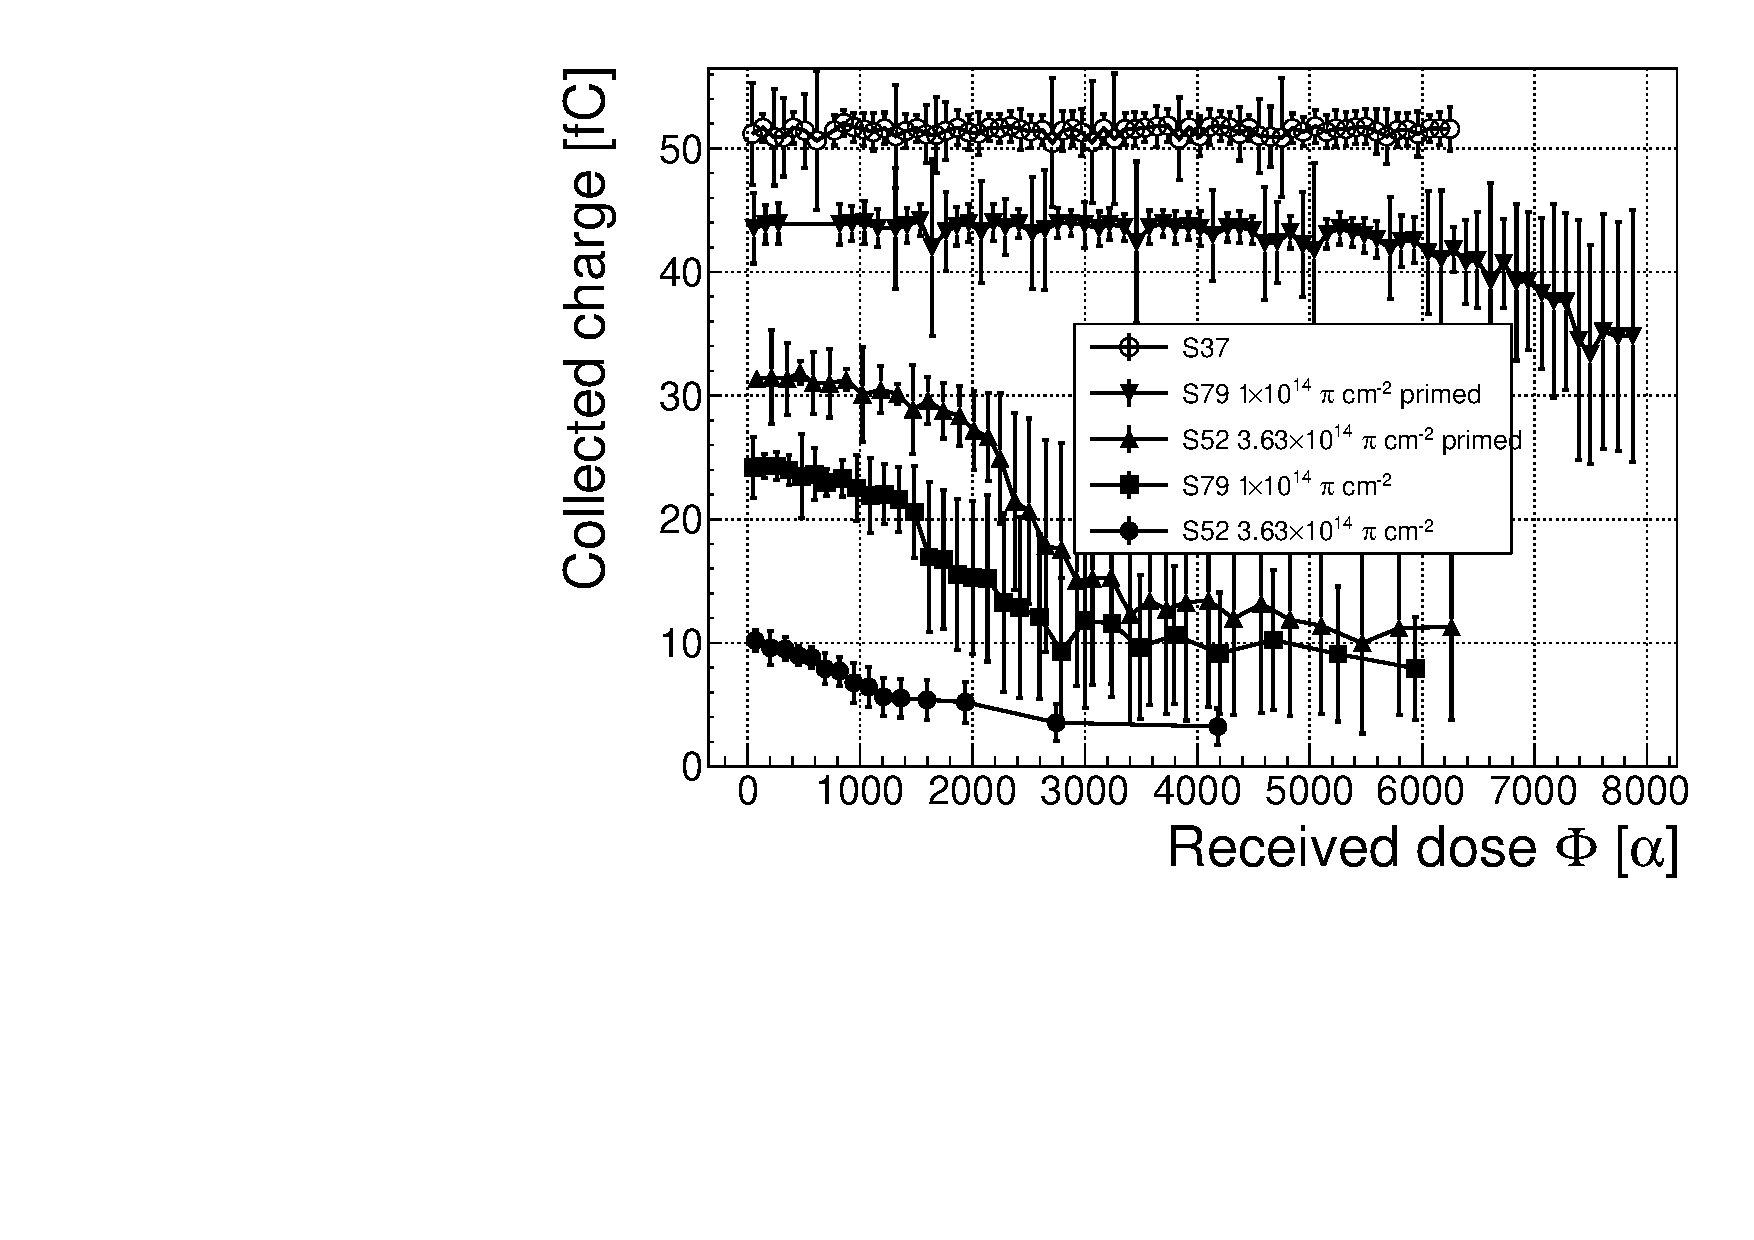
\includegraphics[width=0.6\textwidth]{scripts/plots/amplvstimecx}
\caption{Comparison of collected charge with time for non-irradiated and irradiated diamond samples.}
\label{fig:longtermcx}
\end{center}
\end{figure}

The next step was to observe the behaviour of the current pulse shapes with time using a C2 current amplifier. The shape of the pulse holds more information about the micro-processes in the sensor than solely the value of the integrated charge. This time only the primed sensors were tested. Both hole and electron collection were observed to determine whether they behave differently or not. The samples were measured long enough for the pulse shapes to start changing. The data show that the pulses start changing in a chaotic way -- suddenly there are several different shapes, some still the same as at the beginning while the others with almost zero amplitude. These data are difficult to interpret. Nevertheless, the idea is that some charges get trapped in the charge traps in the bulk for a long time, building up regions of space charge. Since only one charge flavour is drifting through the bulk whereas the other is quickly recombined, this already determines the imbalance in spatial distribution of trapped charges. The built up space charge affects the electric field, making it non-uniform. The non-uniform field in turn affects the drifting carriers, slowing them down or speeding them up, depending on the field gradient. Since the movement of the carriers is the electric current, the field gradient can be observed in the signal. Unfortunately the effects are very convoluted, probably due to the impinging point of the $\upalpha$ particle. 

TO-DO show the degrading pulses. PLOT!

Finally, an effort has been made to find a way for the pulse shapes to return to their initial state. Three methods were tested: 1) Priming with $\upbeta$ at bias voltage applied, 2) priming with $\upbeta$ without bias voltage and 3) priming with $\upgamma$ without bias voltage. It turns out that the first method degrades the shapes further. This effect has already been described in~\cite{Kramberger}. The second and third method, however, improve the pulse shapes. The "healing" process depends on the radiation rate and the time of exposure. The ionising radiation creates free charges, which quickly recombine close to the place of generation. It is likely that they also release the charges trapped during the measurement, reducing the overall effect of the space charge. The traps get filled with both flavours of carriers, thus neutralised. The pulse shape returns to its initial state.

TO-DO show the healing process. PLOT!

TO-DO conclusions: limitations


%% sample landau distribution  
%\begin{figure}[!t]
%\begin{center}
%%\includegraphics[width=0.6\textwidth]{}
%\caption{Change of the pulse shape with time. PLACEHOLDER}
%\label{fig:landausample}
%\end{center}
%\end{figure}



%\begin{figure}[!t]
%\begin{center}
%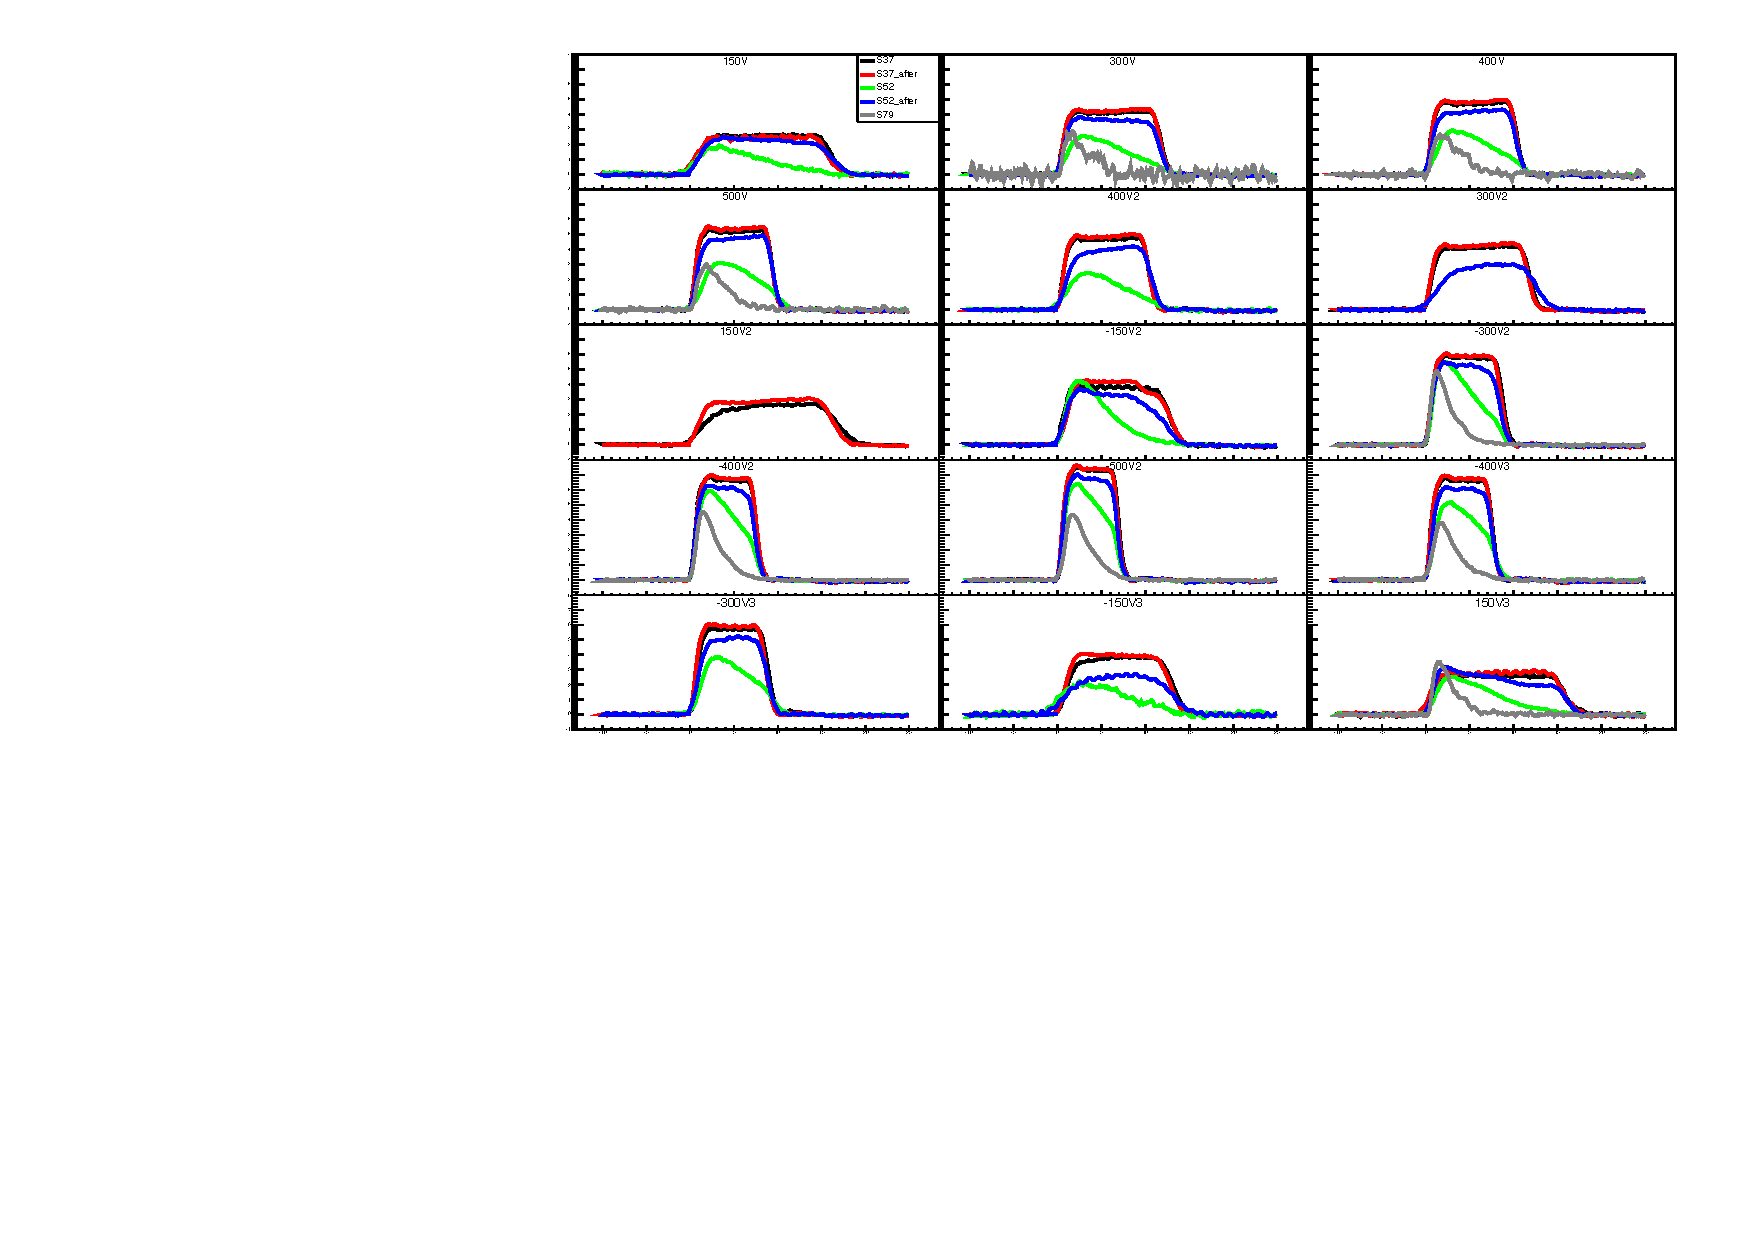
\includegraphics[width=1\textwidth]{plots/hysteresis/all_pulses_1}
%\caption{S37 non-irrad; S52 $1\times10^{14}~p~cm^{-2}$ non-pumped, pumped; S79 $3.63\times10^{14}~p~cm^{-2}$ non-pumped, pumped PLACEHOLDER}
%\label{fig:hystall}
%\end{center}
%\end{figure}















% ---------------------------------------------------------------------------------------------------------------
%\clearpage
\section{Temperature limitations}
\label{sec:templimit}
% ---------------------------------------------------------------------------------------------------------------
A test was carried out to evaluate the effect of temperature changes on the output signal of the diamond sensors. A cryostat filled with liquid helium was used to cool down the sensor during the measurement process. Current signal response to $\alpha$-particles was measured at 18 temperature points between 4~K and 295~K (room temperature - RT). At every temperature point, a set of 300 pulses was read out at various bias voltages. Resulting data showed that the charge collection is stable down to 150~K, where it starts decreasing and stabilises again at about one third of the initial value at 75~K. This behaviour was first measured and discussed by H. Jansen in~\cite{JansenThesis}.

%\subsubsection{Acoustic phonon scattering}
The band gap energy in diamond equals to $E_g=5.5$~eV while the average energy to produce an electron-hole pair is $E_{e-h}=13.25$~eV. This means there is excessive energy deposited in the diamond bulk. The impinging $\upalpha$-particle stops within $\sim$10~$\upmu$m of the bulk, transferring all its energy to the lattice. A part of this energy, approximately 40~\%, directly ionises the carbon atoms, creating free electron-hole pairs. The remaining energy, however, is converted into lattice vibrations (phonons~\cite{Phonons}). This effectively means that the lattice within the ionisation volume (approximately $\sim$10~$\upmu$m$\times\sim$2~nm in size) is briefly heated up. The hot plasma then cools down to the temperature of the surrounding material by heat dissipation, (i.e. phonon transport).

%\subsubsection{Exciton formation and recombination}
The positively charged hole and negatively charged electron in the hole attract each other via the Coulomb force and may undergo a bonding process during which a phonon is emitted. That phonon is referred to as \emph{exciton}~\cite{Exciton}. The electron is pushed to a so-called exciton energy band, which is 80~mV under the conduction band. At higher temperatures, the lattice provides enough energy to excite the electron from the exciton state back to the valence band (so-called exciton recombination). At lower temperatures, however, the exciton lifetime increases, which means that it will take a longer time for the electrons to get re-excited to the valence band. The re-excitation lifetime at room temperature is $\sim$30~ps, increasing to $\sim$150~$\upmu$s at 50~K.
%The irradiated samples were put in the cryostat, which was cooled down to 4.2~K using liquid helium. TCT data were then taken at a range of bias voltages at temperature points ranging between 4.2~K and room temperature (RT). The results showed that irradiation causes forming of charge traps in the bulk.l;'
%
%TO-DO: get the Tau and plot it against T. 
%TO-DO: plot the drift time against square voltage.


\subsection{Temperature-variant $\upalpha$-TCT before irradiation}
% Show a set of pulses
Three sCVD diamond samples were tested at the range of temperatures using the $\upalpha$-TCT technique. At each temperature point, the bias voltage was set to several positive and negative values. A set of 300 pulses was recorded at every data point and averaged offline. The resulting averaged pulses of sample S37 at the 260~K temperature point and a bias voltage of $\pm$400~V, $\pm$500~V and $\pm$700~V are shown in figure~\ref{fig:voltpulse}.  The pulses induced by holes as charge carriers are shorter than those induced by electrons, confirming that holes indeed travel faster in diamond. The area of the pulse, however, is the same for both polarities, which corresponds to the fact that the same amount of charges is drifting in both cases.

\begin{figure}[!t]
\begin{tabular}{rr}
\subfloat{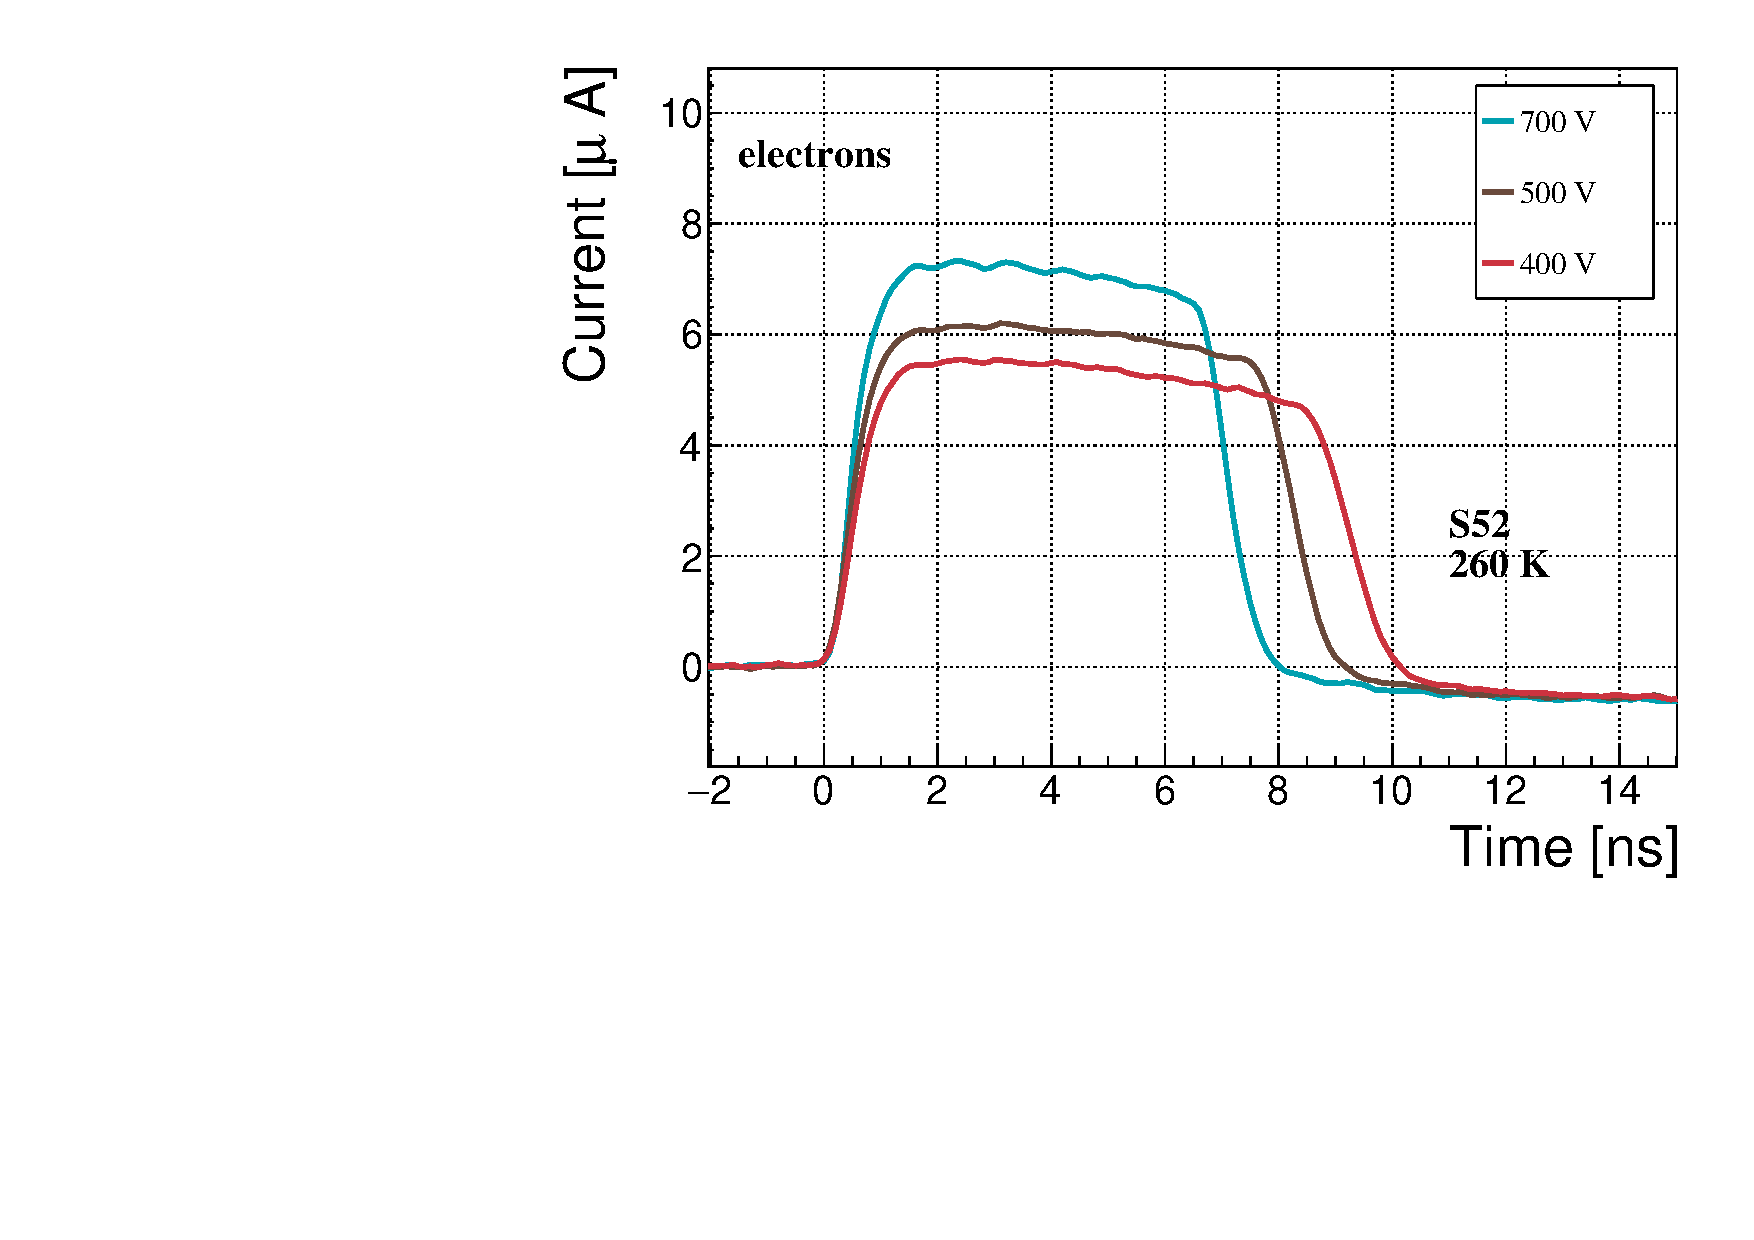
\includegraphics[width=0.47\textwidth]{scripts/plots/pulsesVolt/varVolt_S52_elecs_260k} \label{fig:S52cTplus}} &
\subfloat{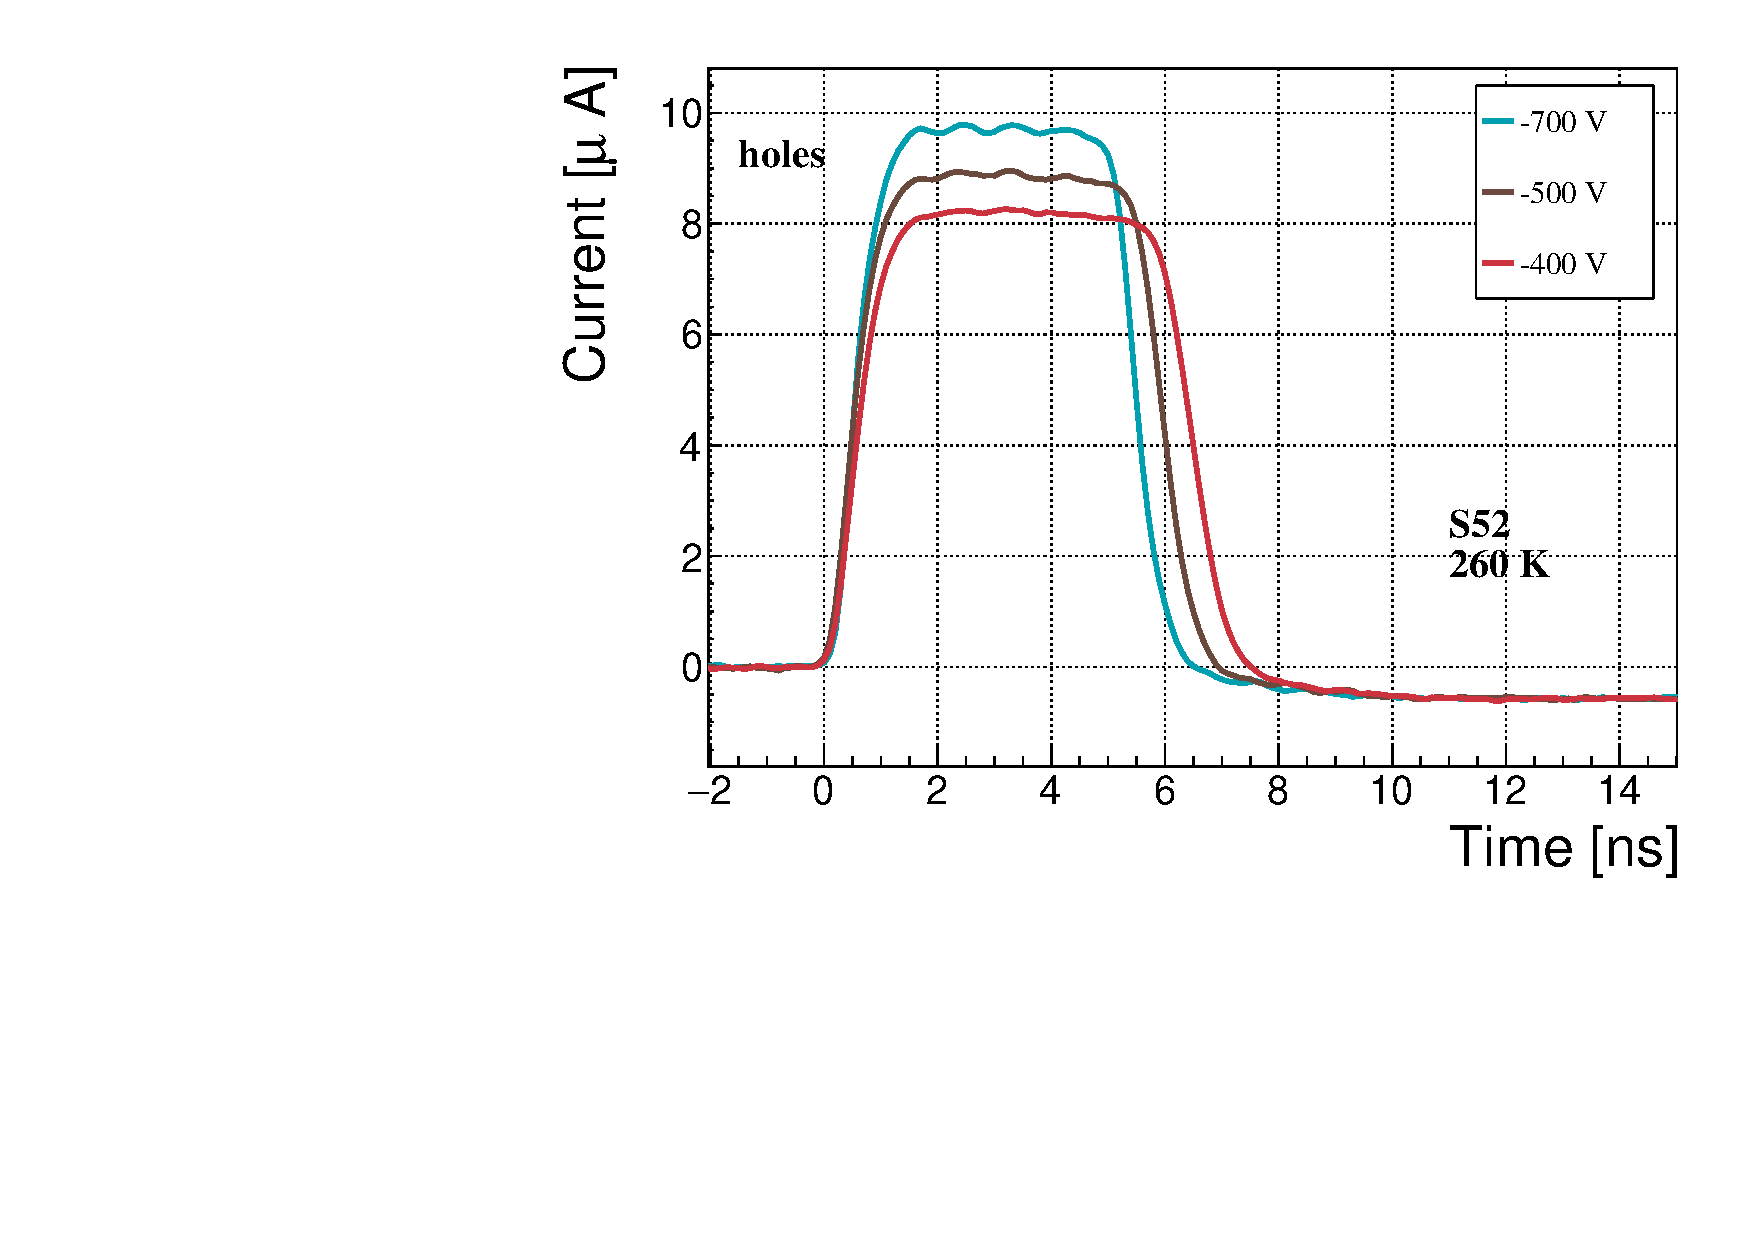
\includegraphics[width=0.47\textwidth]{scripts/plots/pulsesVolt/varVolt_S52_holes_260k}  \label{fig:S52ctTminus}}
\end{tabular}
\caption{Varied bias voltage at a fixed temperature}
\label{fig:voltpulse}
\end{figure}

Figure set~\ref{fig:temppulses} shows pulses at bias voltage set to $\pm500$~V across the range of temperatures between 4~K and 295~K -- room temperature (RT). Several conclusions can be drawn by observing their shape. First, the pulse shapes change with decreasing temperature. The pulse time gets shorter, hinting at the faster carrier drift velocity $v_{drift}$. Second, between 150~K and 75~K there is a significant change in shape - the time constant of the rising edge increases significantly and the pulse area decreases. From 75~K down to 4~K there is no significant observable change. Last, the top of the pulse at the S52 is not flat, which means that a portion of the drifting charge is lost along its way. This could be due to impurities in the diamond bulk, which act as charge traps, or due to the space charge built up in the bulk. A linear pulse top hints on the latter. All in all, the pulse shape changes significantly with temperature, which is predicted by Jansen's model.

\begin{figure}%[!t]
\begin{tabular}{rr}
\subfloat{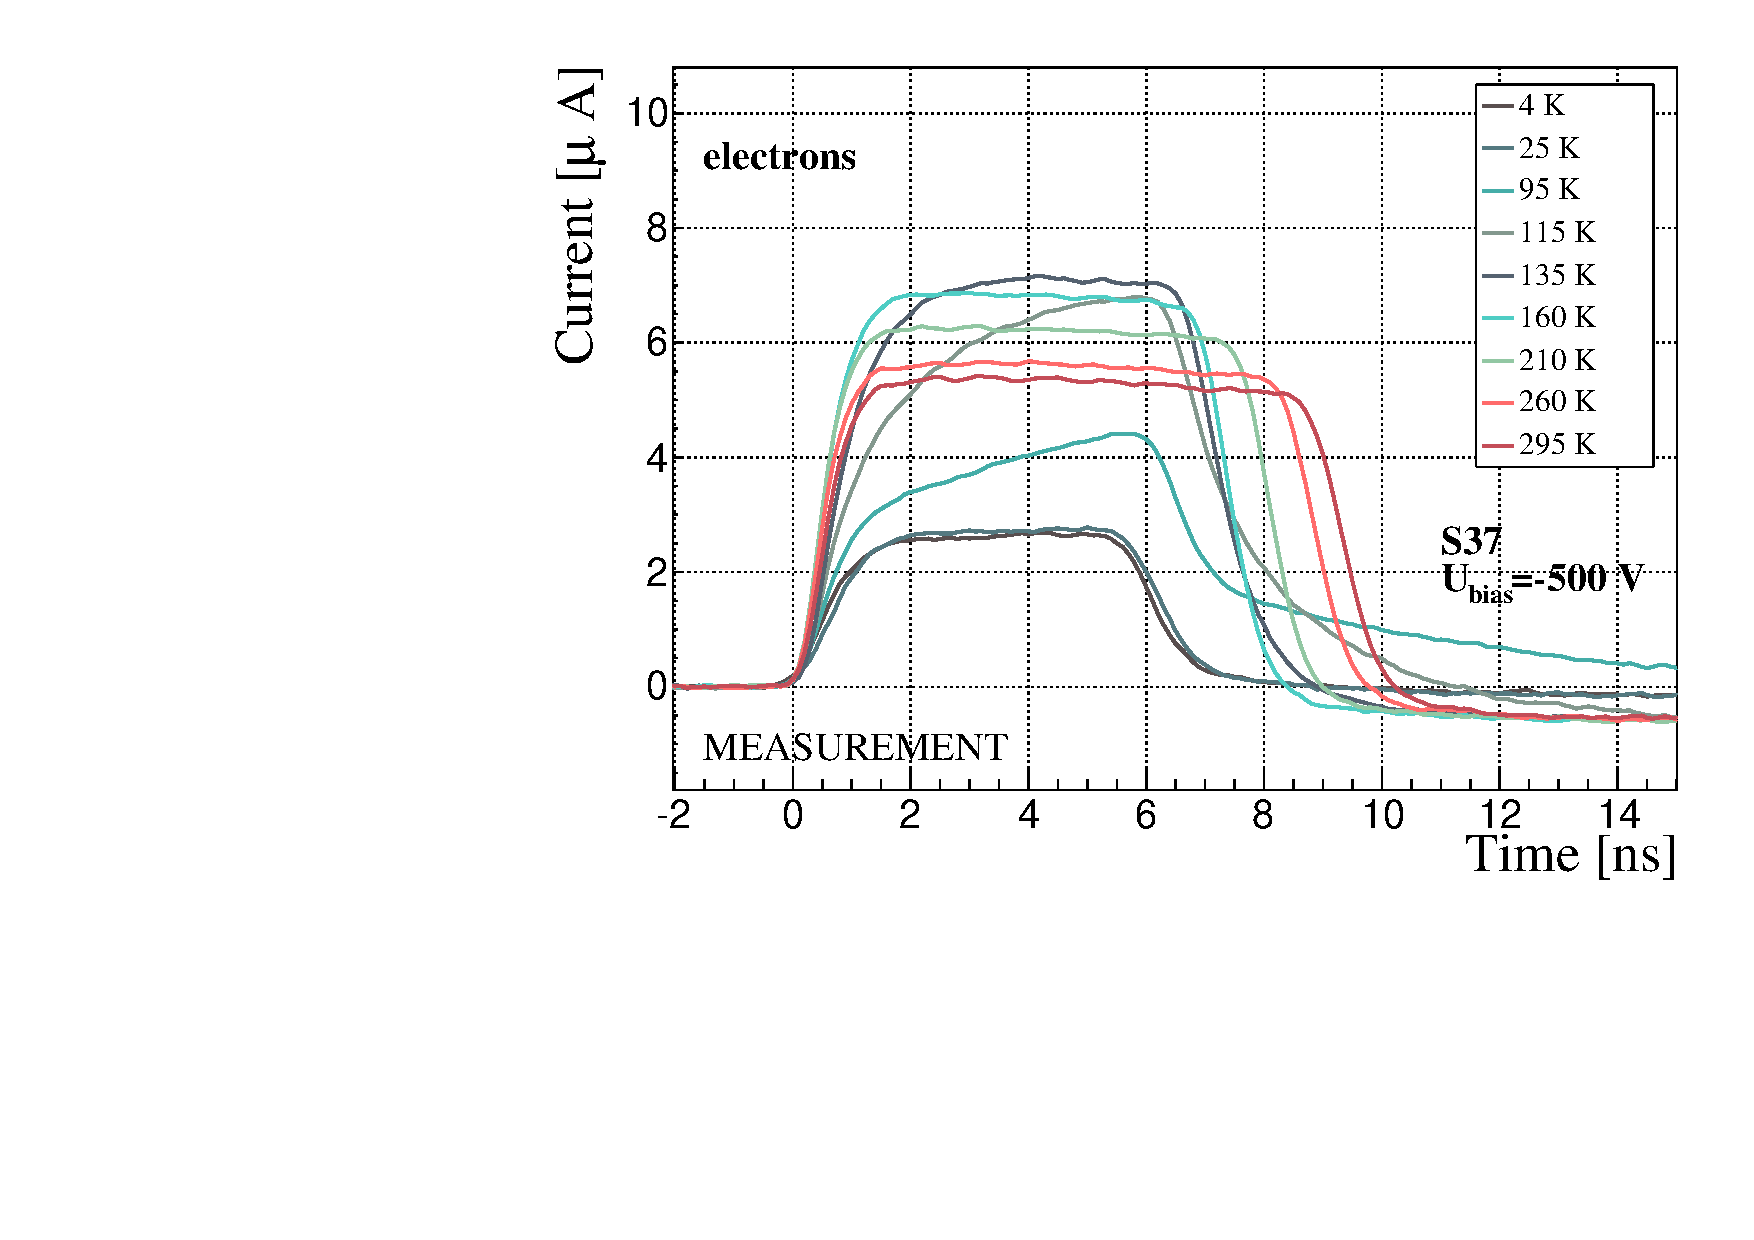
\includegraphics[width=0.47\textwidth]{scripts/plots/pulses/S37_elecs} \label{fig:S37plus}} &
\subfloat{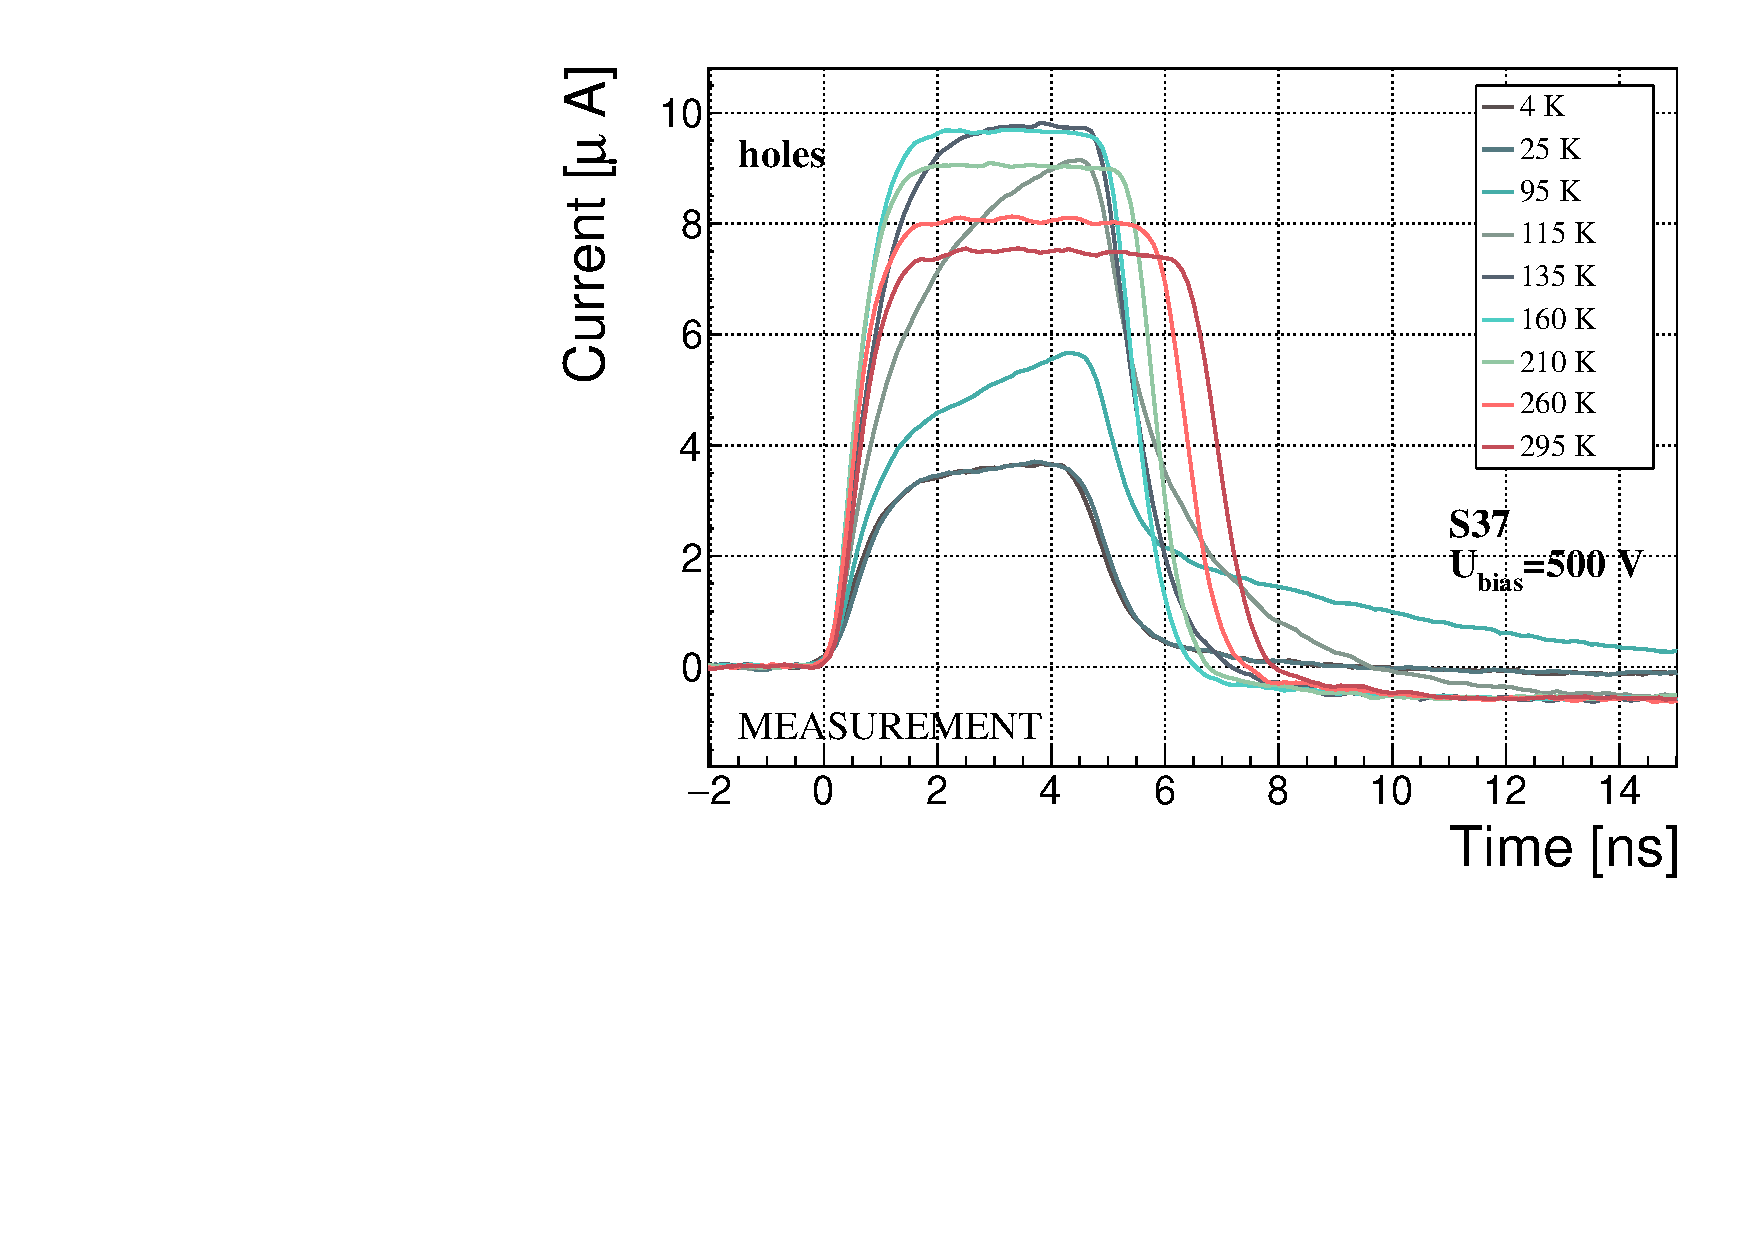
\includegraphics[width=0.47\textwidth]{scripts/plots/pulses/S37_holes}  \label{fig:S37minus}} \\
\subfloat{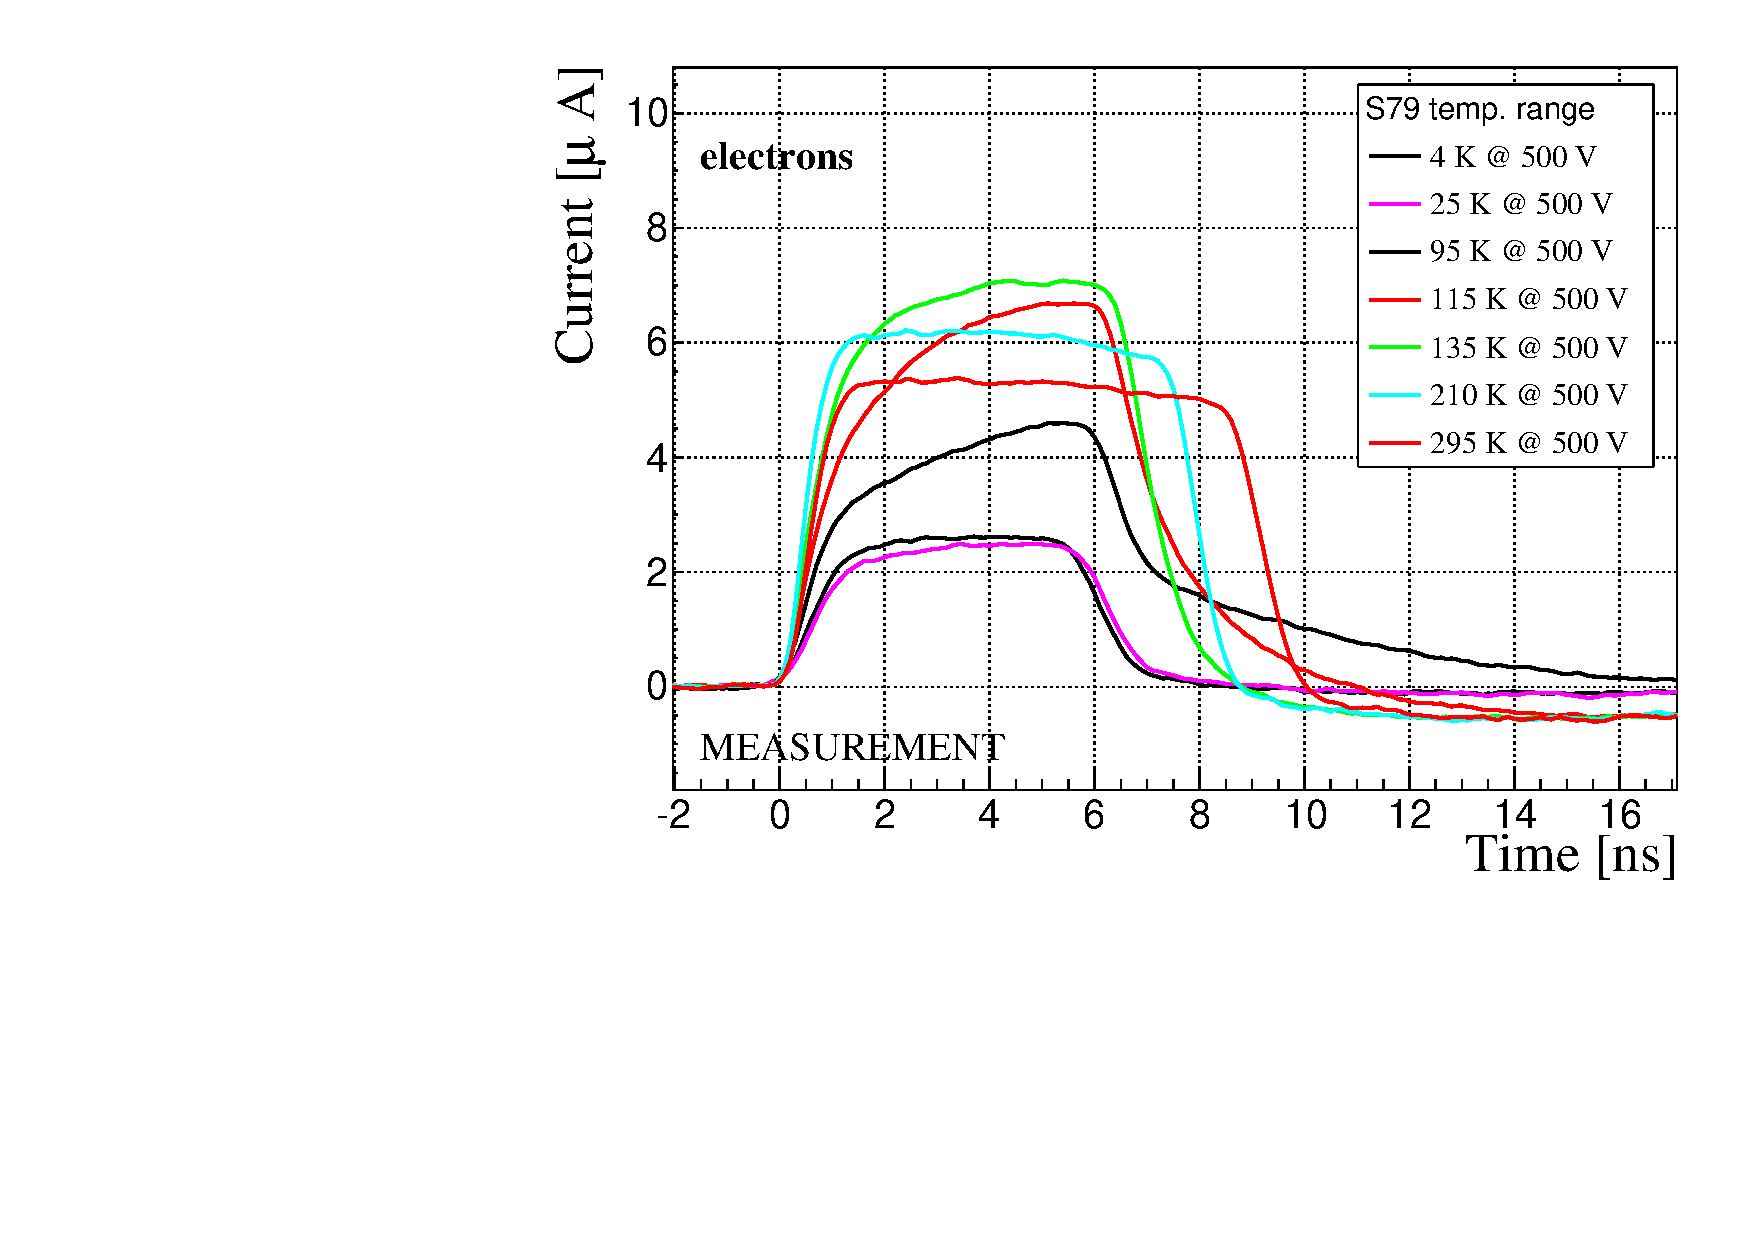
\includegraphics[width=0.47\textwidth]{scripts/plots/pulses/S79_elecs} \label{fig:S79plus}} &
\subfloat{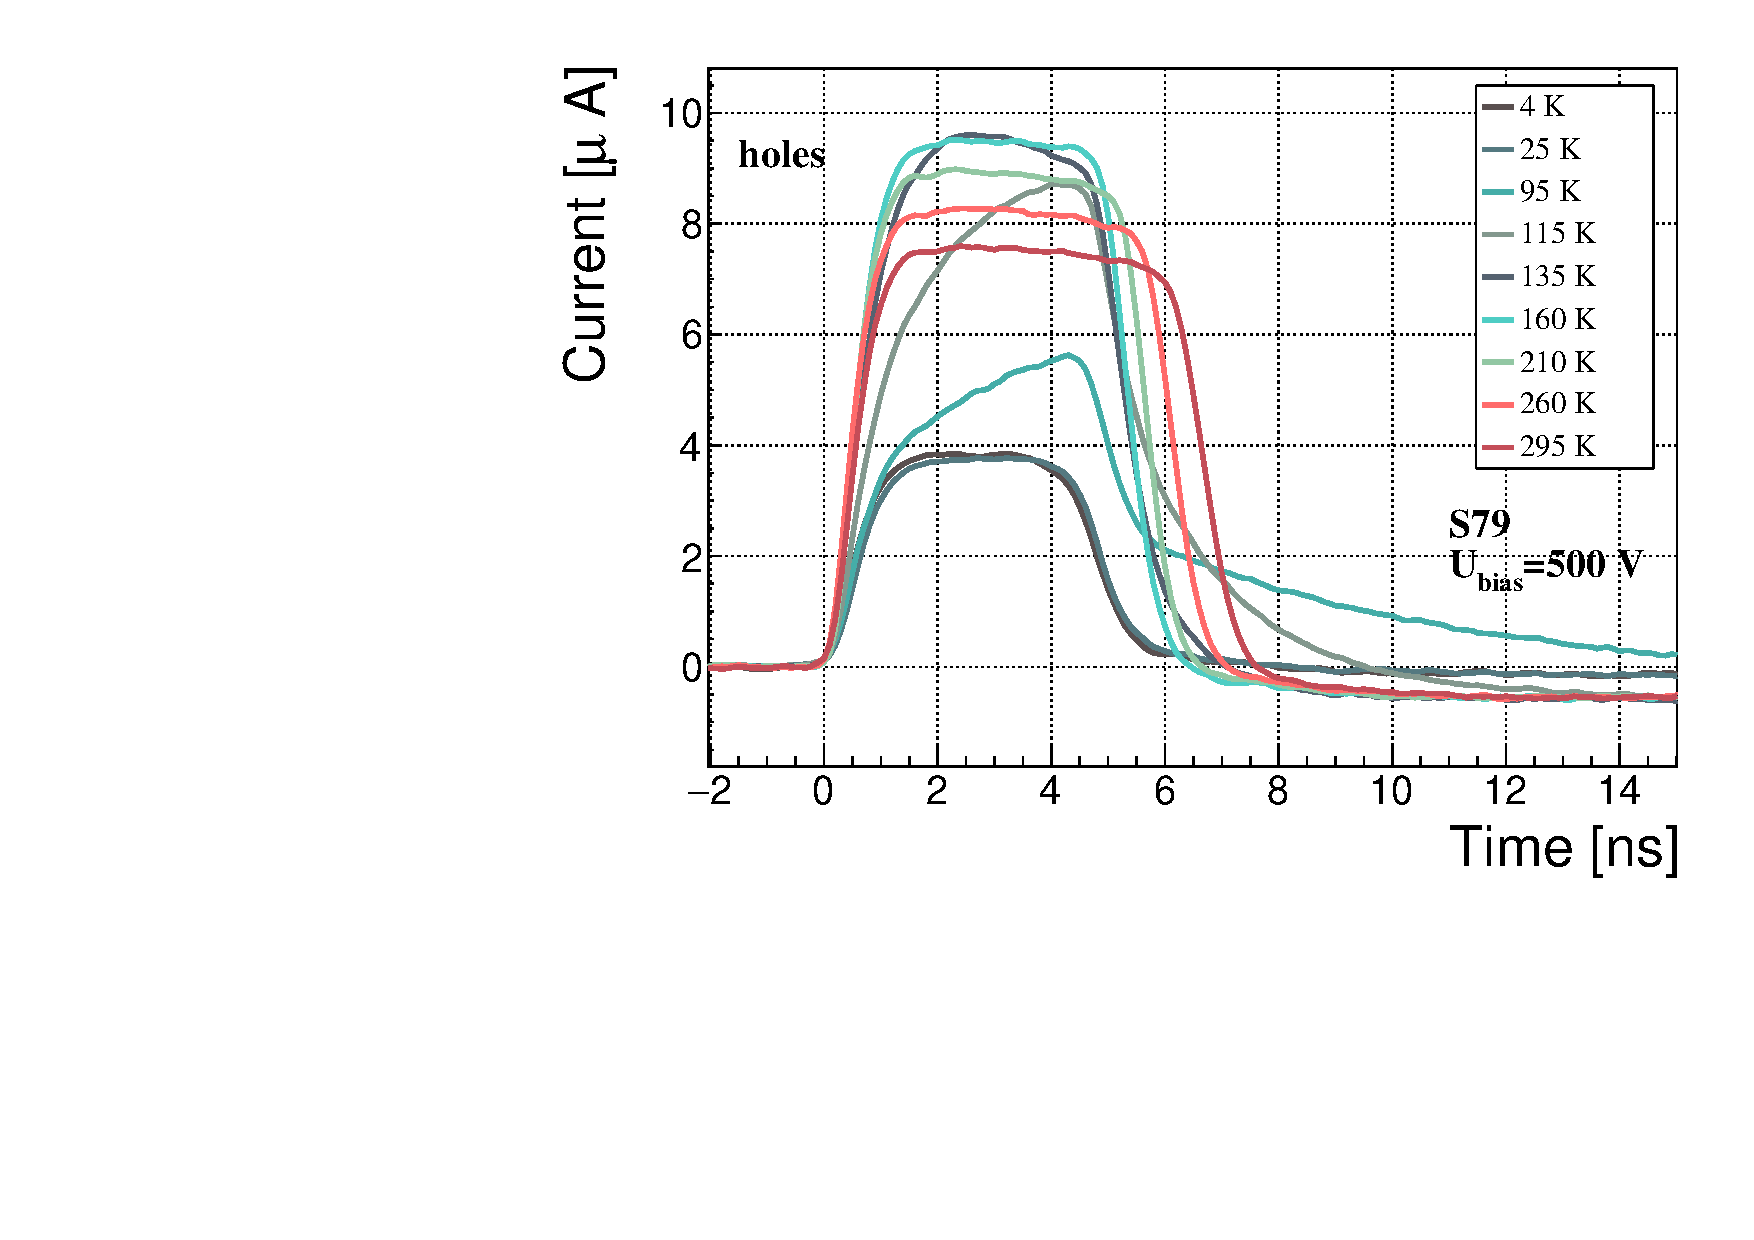
\includegraphics[width=0.47\textwidth]{scripts/plots/pulses/S79_holes}  \label{fig:S79minus}} \\
\subfloat{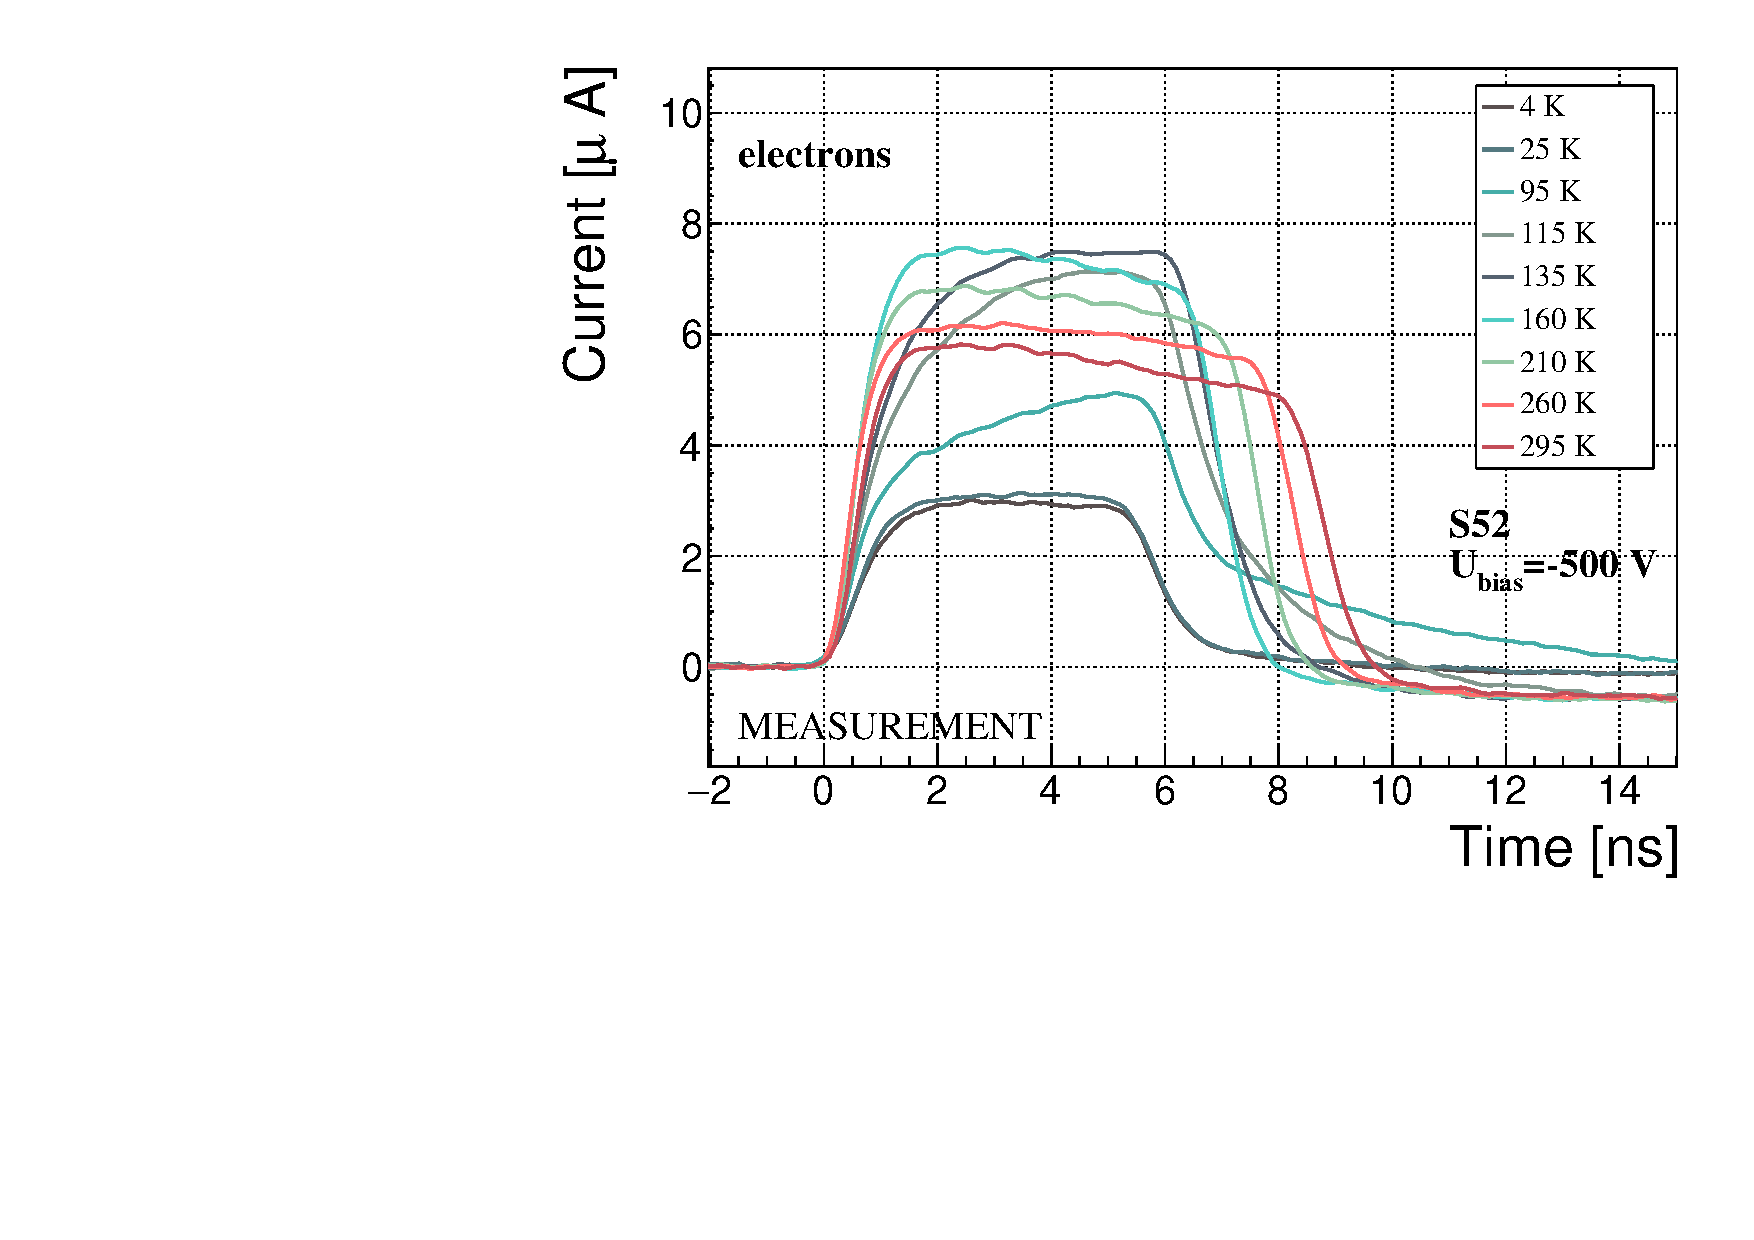
\includegraphics[width=0.47\textwidth]{scripts/plots/pulses/S52_elecs} \label{fig:S52plus}} &
\subfloat{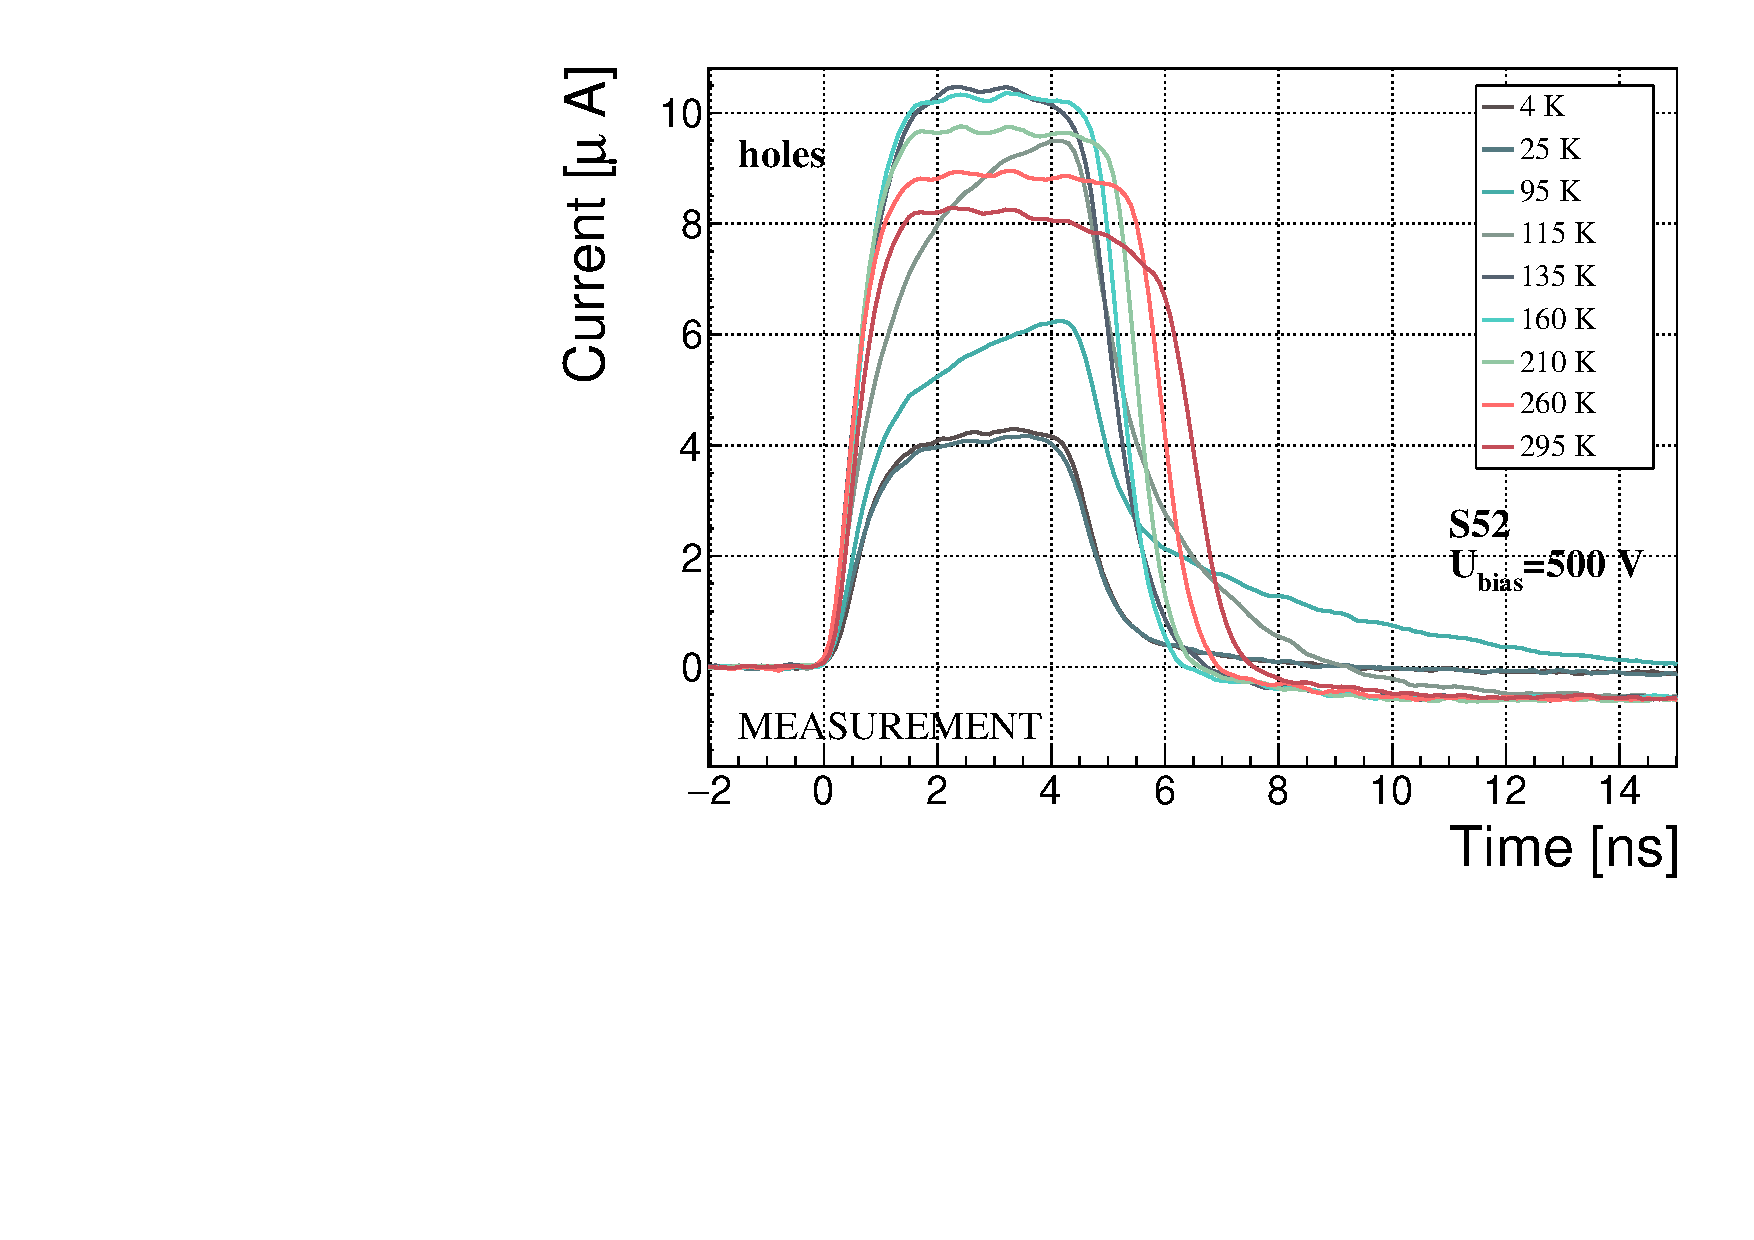
\includegraphics[width=0.47\textwidth]{scripts/plots/pulses/S52_holes}  \label{fig:S52minus}}
\end{tabular}
\caption{Several data points between 4~K and 295~K at a bias voltage of $\pm$500~V}
\label{fig:temppulses}
\end{figure}


% TO-DO Show drift velocity wrt volt
% TO-DO Show drift velocity wrt temp
% TO-DO Show integrated charge
% TO-DO Show Vdrift wrt 1/Voltage
%$(1\pm0.2)\times10^{14}~\pi~cm^{-2}$ and $(3.63\pm0.76)\times10^{14}~\pi~cm^{-2}$. 

\subsection{Temperature-variant $\upalpha$-TCT after irradiation}
The irradiated S79 and S52 were re-tested in the cryostat. The aim was to see how their pulse shapes change with decreasing temperature, in particular the decaying top of the pulses (see figure~\ref{fig:voltpulseAfter}). The decay time gives information on trapping of charge carriers while travelling through the diamond bulk. A variation of the decay time constant as a function of temperature might help to reveal the type and depth of the charge traps. To observe these effects (or lack thereof), a number of requirements had to be met. First, the diamond samples were intentionally not primed prior to the experiment because priming would improve the pulse shapes and the decaying tops. Second, keeping in mind that the pulse shape of irradiated diamonds changes with time, the length of the measurement of an individual data point had to be adequately short. Last, the sequence of the bias voltage settings was important, the reason for which is explained below.

Unfortunately it was not possible to avoid temporal pulse changes. For instance, one measurement point took approximately one minute. After the measurement, the bias voltage polarity was swapped for a few seconds to bring the diamond back into its initial state. But a few seconds with respect to a minute was not enough. Therefore, when the bias voltage was set to the next value, there was still some residual effect of the previous measurement. Similar to the effects of polarisation, this effect was also decreasing the pulse height. This can be observed in figure~\ref{fig:voltpulseAfter}, which shows the resulting pulses of S52 for bias voltages of $\pm$200~V, $\pm$300~V, $\pm$400~V and $\pm$500~V at 230~K and 260~K. In this case the measurements sequence was: 230K (200~V, 300~V, 400~V, 500~V, -500~V, -400~V, -300~V), 260~K (-200~V, -300~V, -400~V, -500~V, 500~V, 400~V, 300~V). The changes in pulse shapes for holes at 230~K and 260~K cannot be attributed to the temperature change. Instead, the explanation could lie in diamond \emph{"polarisation"}. This means that, when exposed to an electric field with $\upalpha$ measurements ongoing, the diamond builds up the internal electric field of inverse polarity, which effectively reduces the overall electric field. This internal field does not dissipate when the external bias voltage is switched off. It can be said that the diamond is "polarised". When switching the polarity of the external bias voltage, the internal and external electric field point in the same direction at the beginning, increasing the overall electric field and with it the pulse height. In figure~\ref{fig:voltpulseAfter}, this happens when switching from 500~V to -500~V at 120~K. The built up polarisation contributes to the pulse having a sharp rising edge and a high amplitude. This effect decays during the next two voltage points. There would be a handful of ways to avoid this polarisation effect in the data: 1) after every data point invert the bias voltage and leave it to return to a neutral state for the same amount of time, 2) make a hysteresis of data points, going from minimum negative to maximum positive bias several times, 3) reduce the measurement time at every bias voltage setting.
Unfortunately, possibility 1 and 2 are very time consuming and would increase the overall experiment time to over one day. The third option would worsen the resulting averaged pulses. In the end an alternative option was chosen: alternating the starting bias voltage and the sequence at every temperature point. With this option, the highest possible systematic error in analysing the pulse shapes could be attained.


\begin{figure}[!t]
\begin{tabular}{rr}
\subfloat{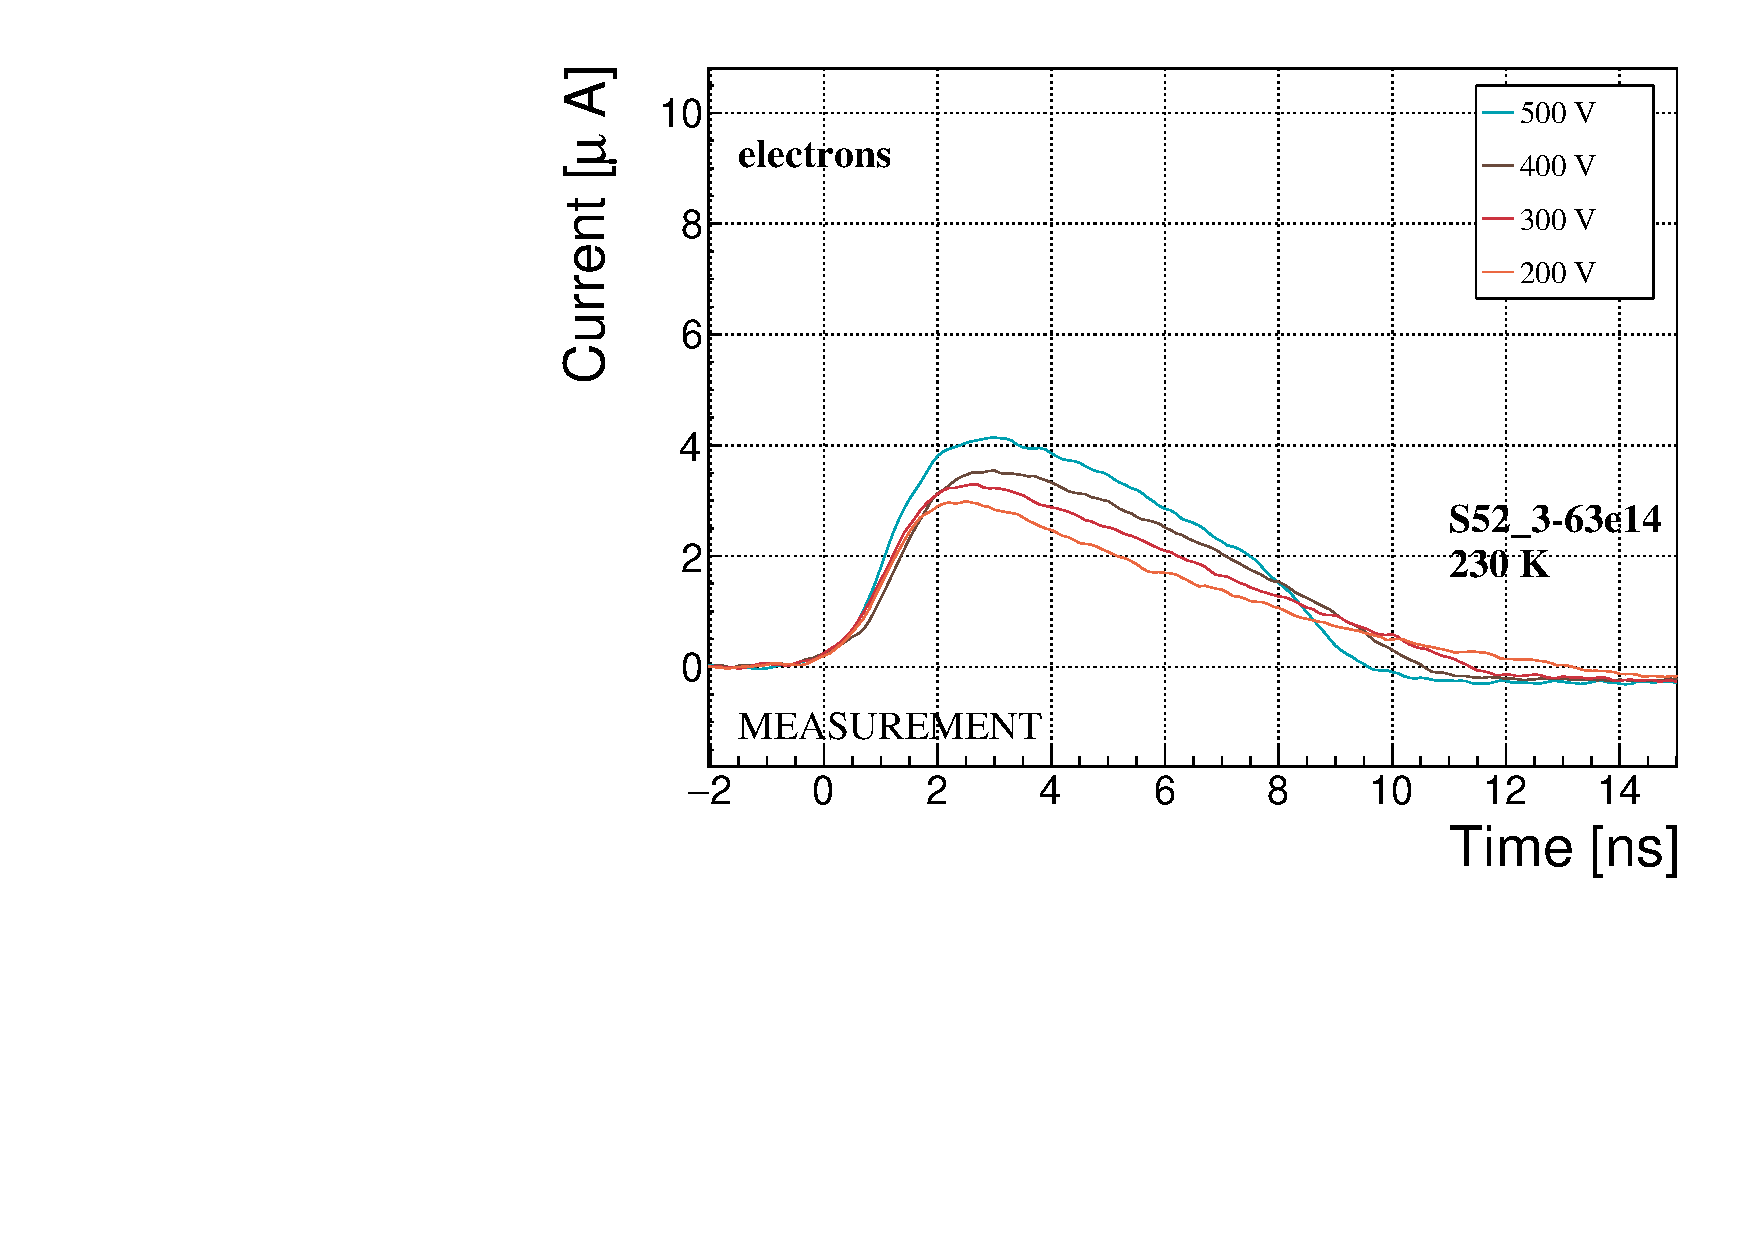
\includegraphics[width=0.47\textwidth]{scripts/plots/pulsesVolt/varVolt_S52_3-63e14_elecs_230k} \label{fig:S52cTplusAfter230}} &
\subfloat{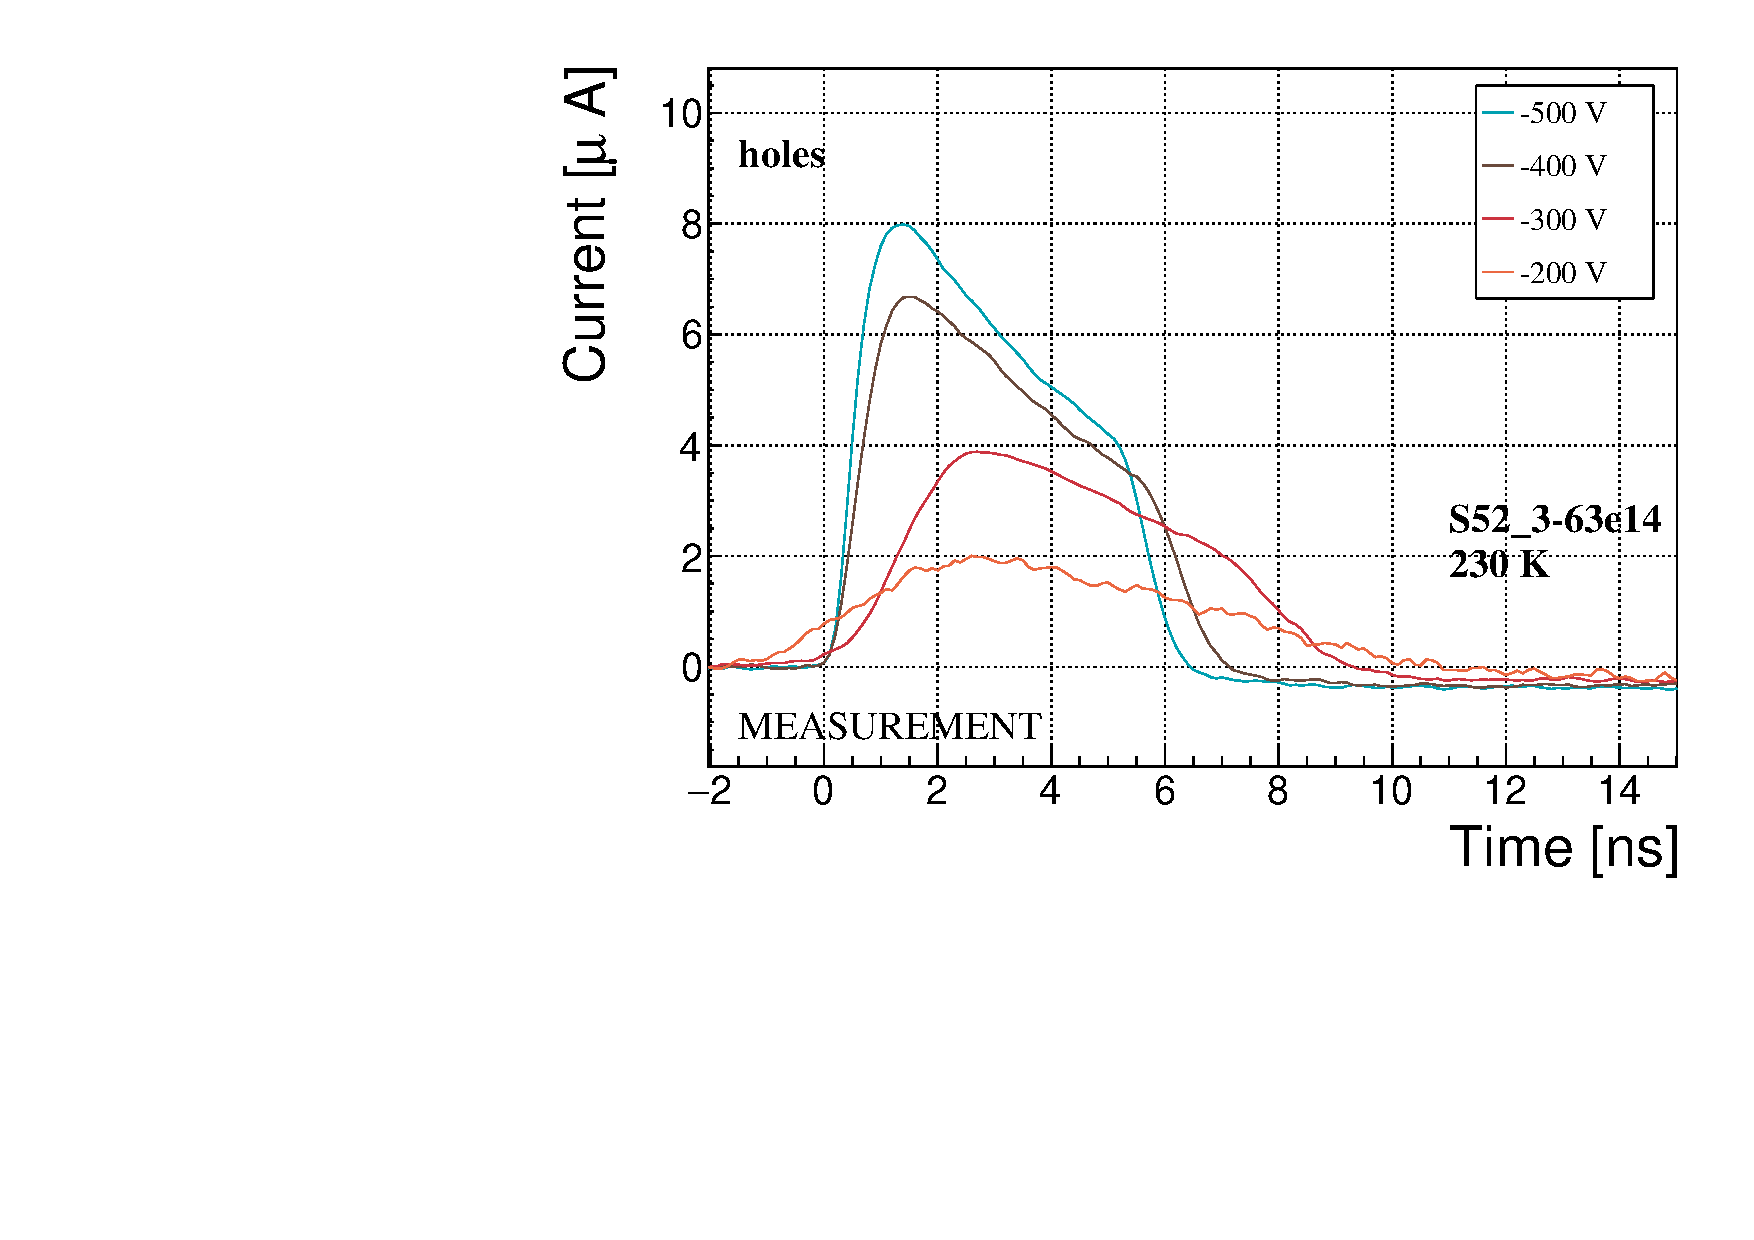
\includegraphics[width=0.47\textwidth]{scripts/plots/pulsesVolt/varVolt_S52_3-63e14_holes_230k}  \label{fig:S52ctTminusAfter230}} \\
\subfloat{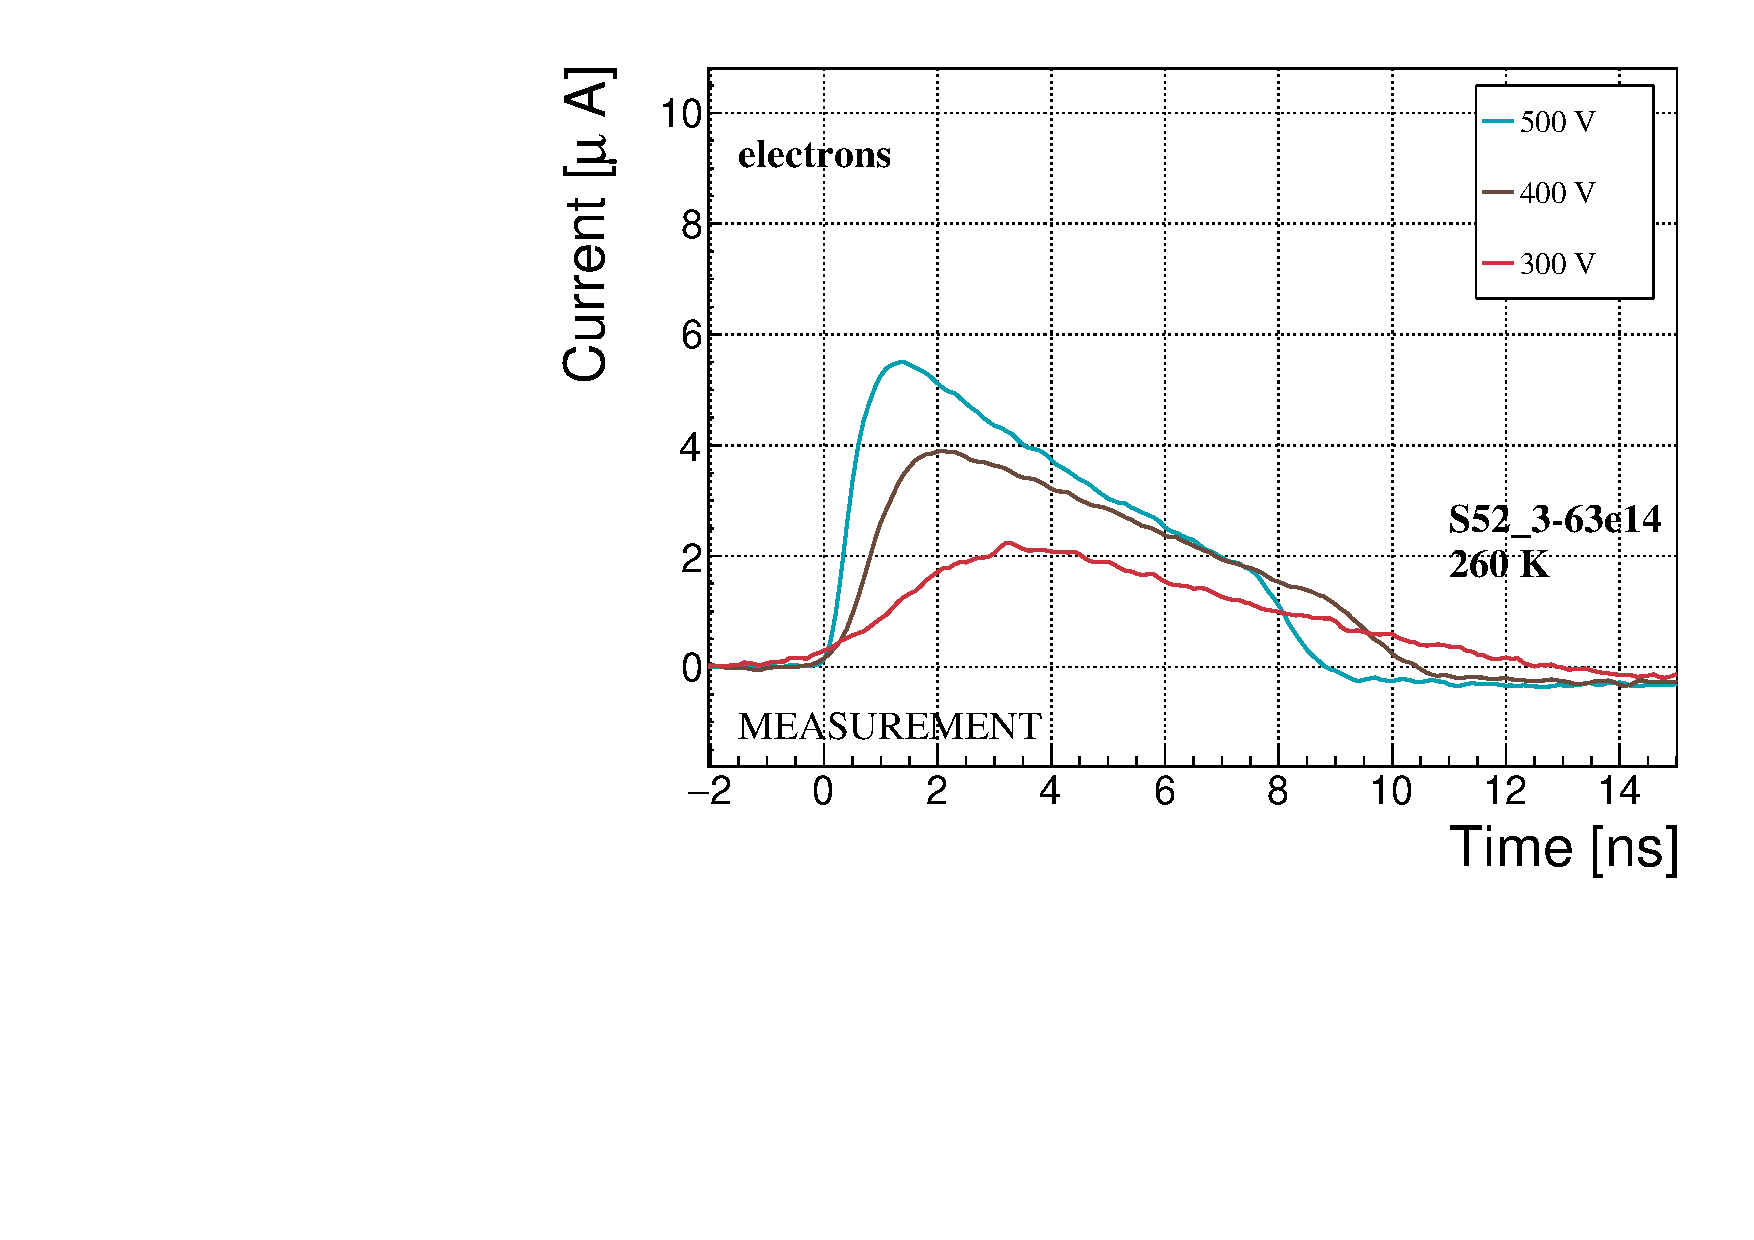
\includegraphics[width=0.47\textwidth]{scripts/plots/pulsesVolt/varVolt_S52_3-63e14_elecs_260k} \label{fig:S52cTplusAfter260}} &
\subfloat{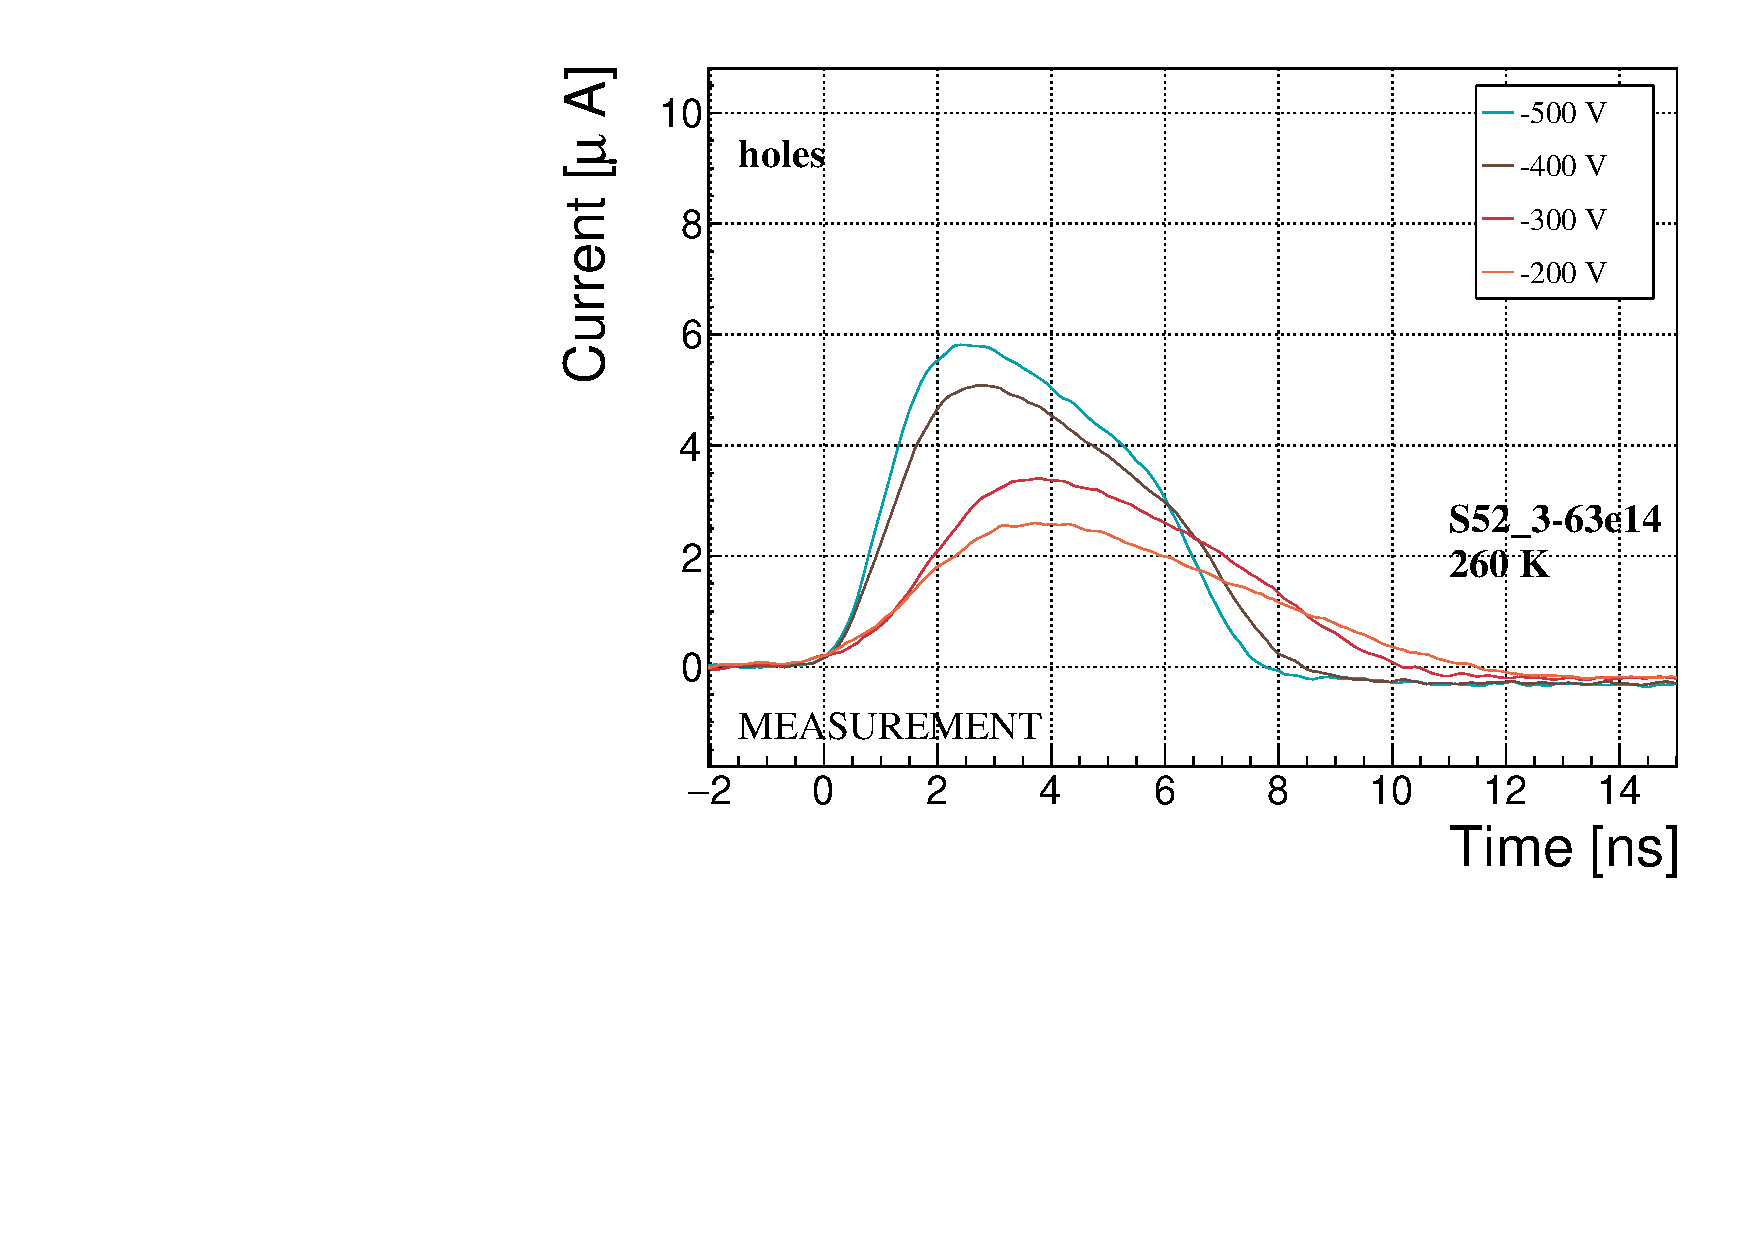
\includegraphics[width=0.47\textwidth]{scripts/plots/pulsesVolt/varVolt_S52_3-63e14_holes_260k}  \label{fig:S52ctTminusAfter260}}
\end{tabular}
\caption{Varied bias voltage at a fixed temperature for an irradiated sample}
\label{fig:voltpulseAfter}
\end{figure}


Figure~\ref{fig:temppulsesAfter} shows the irradiated S52 and S79 as well as the non-irradiated S37 for comparison, all at a bias voltage of $\pm$500~V and at several temperature points between 4~K and RT. It is evident that the irradiation affected the shape of the pulses across all temperatures. 


\begin{figure}[!t]
\begin{tabular}{rr}
\subfloat{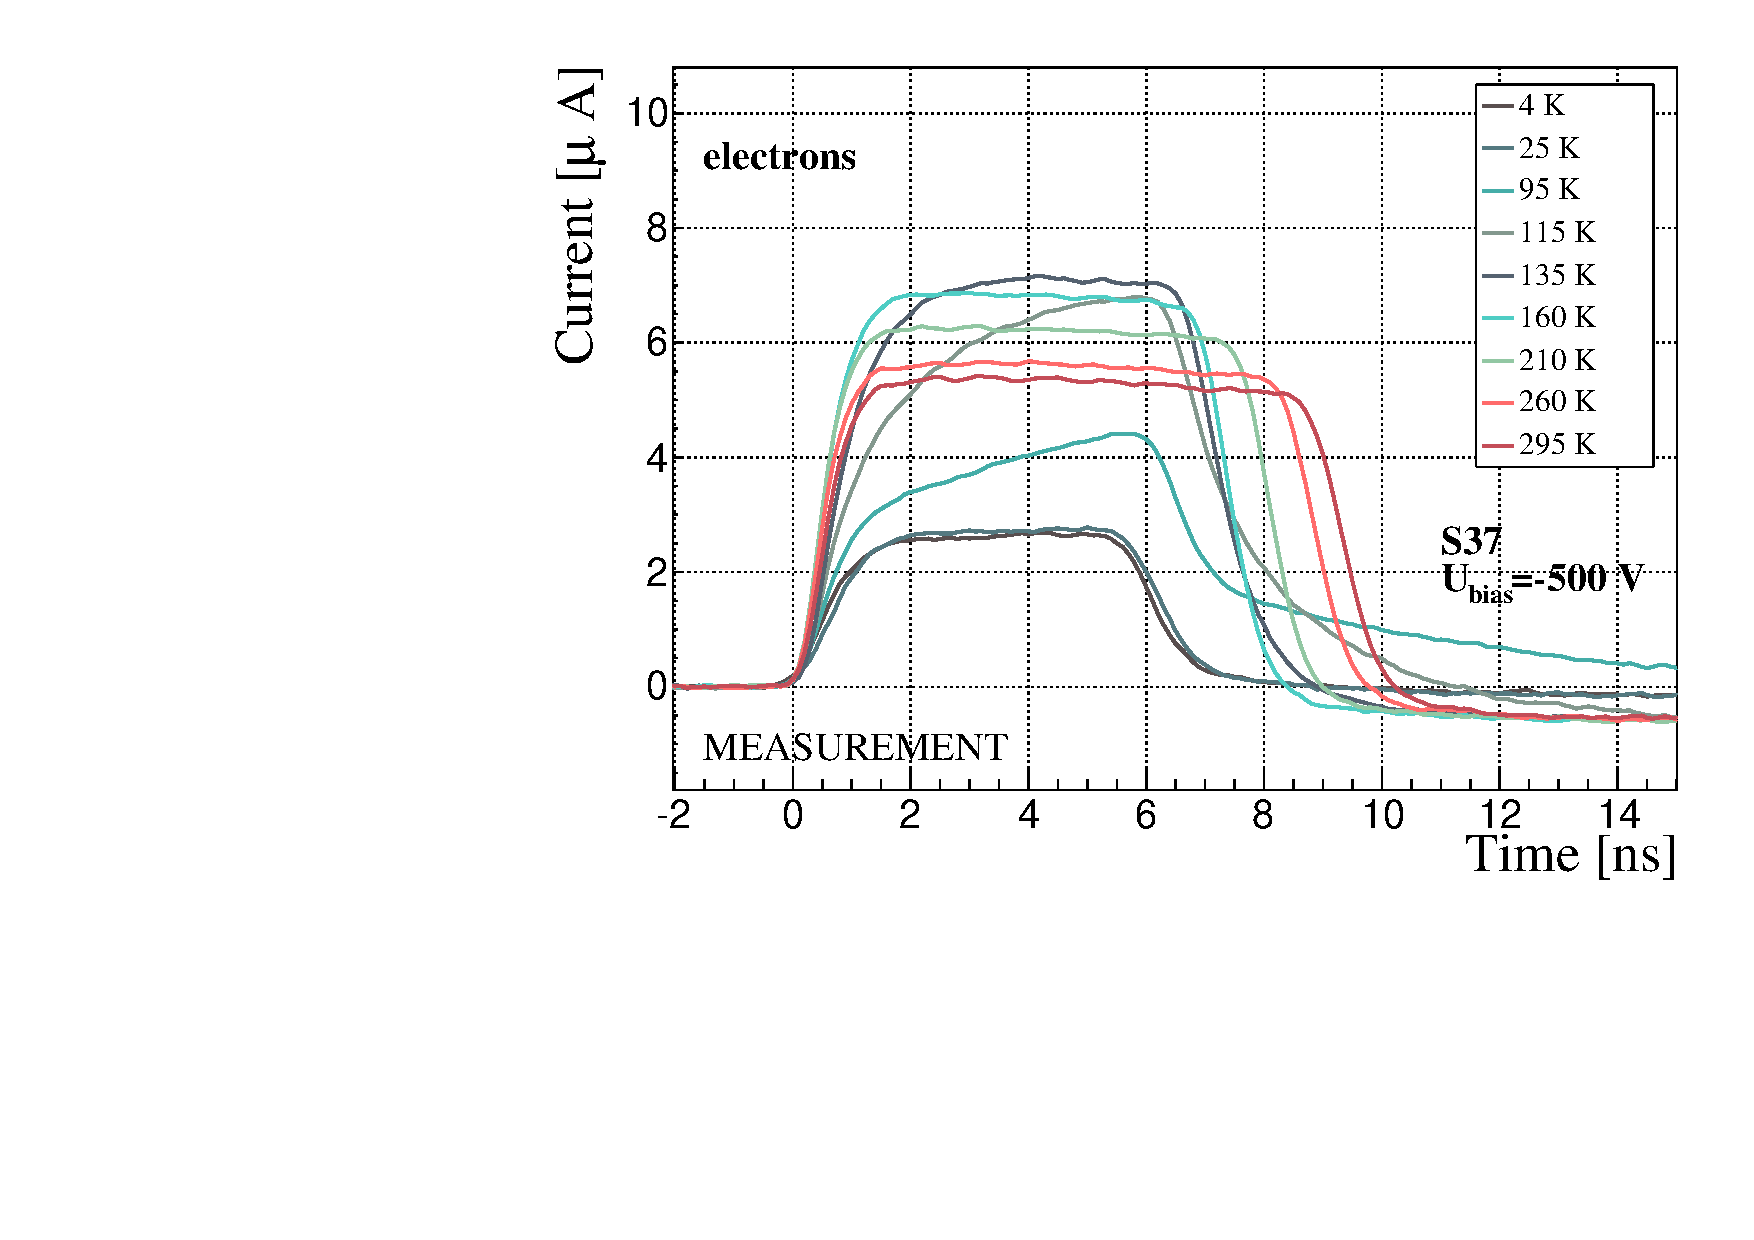
\includegraphics[width=0.47\textwidth]{scripts/plots/pulses/S37_elecs} \label{fig:S37plusAfter}} &
\subfloat{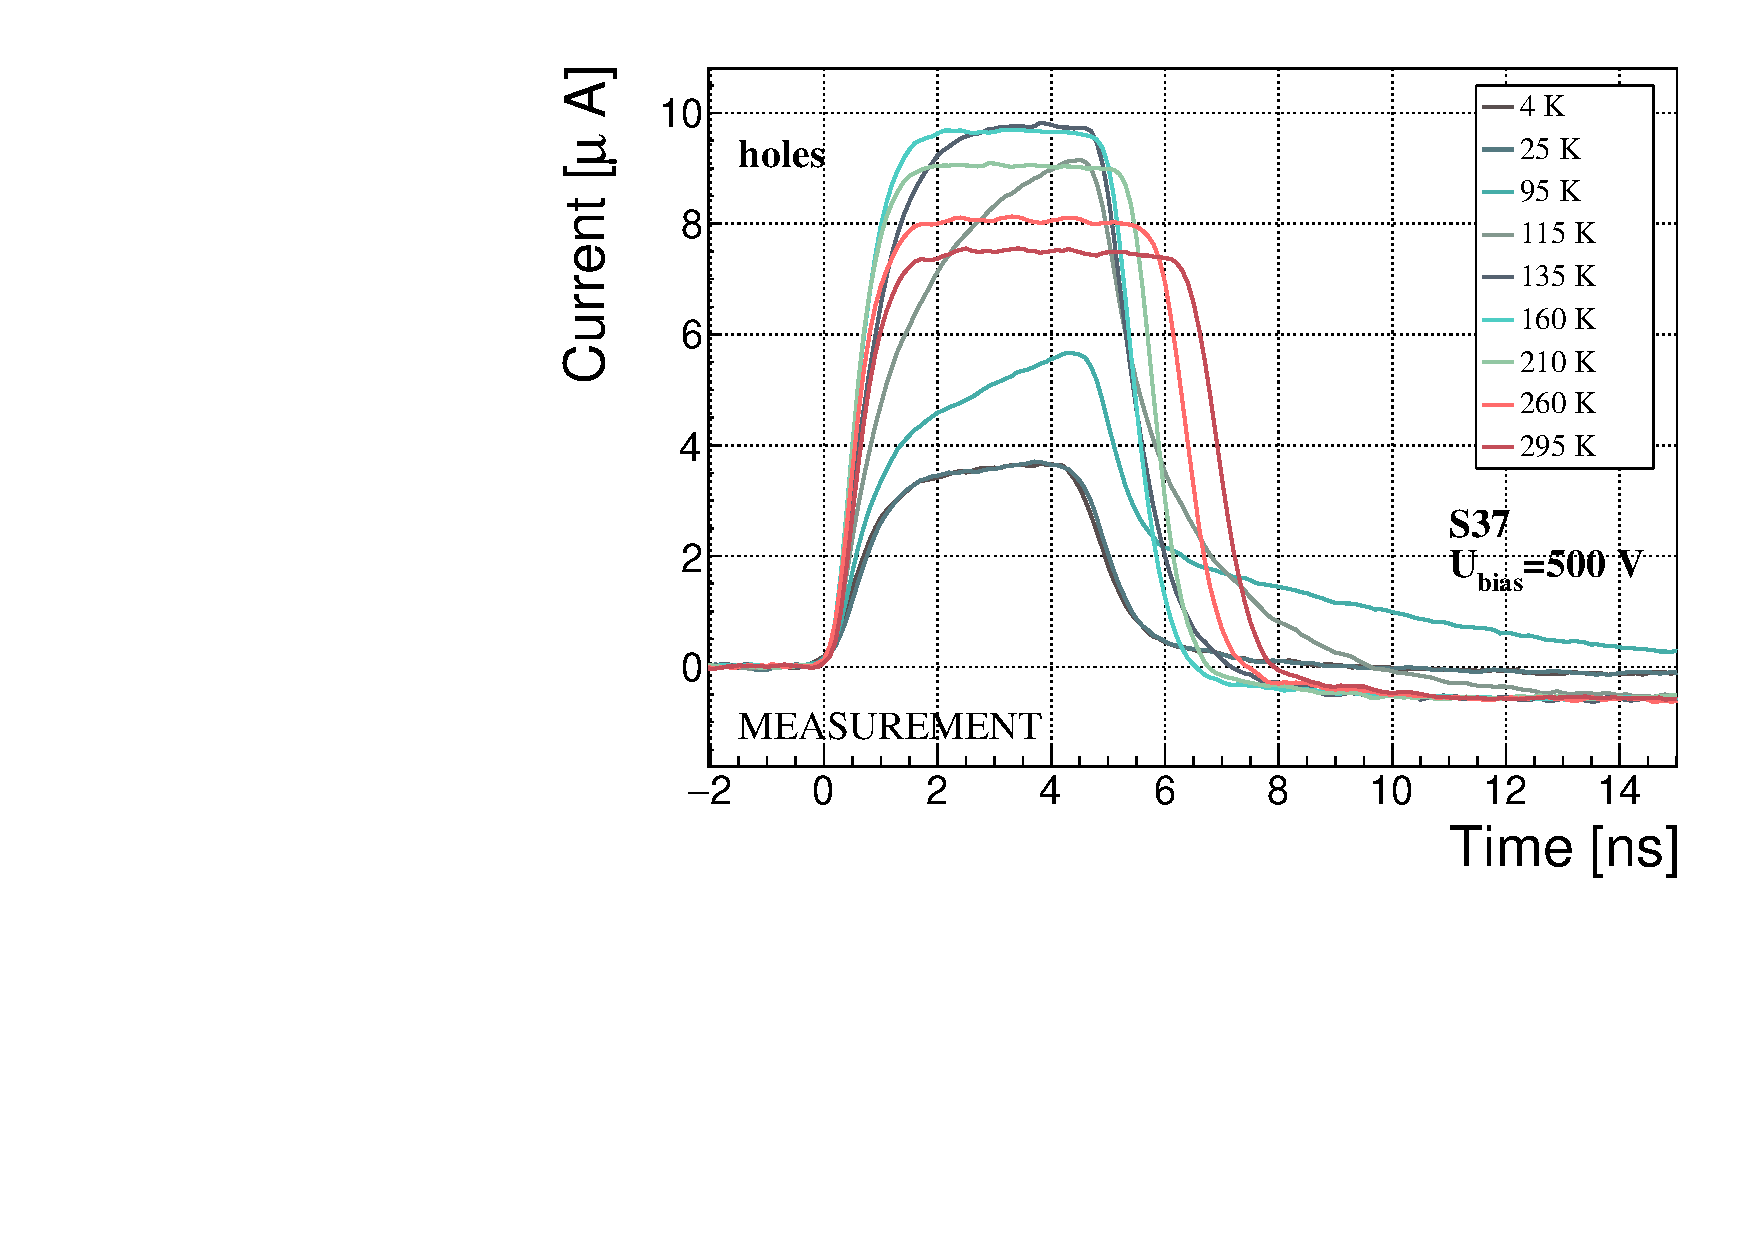
\includegraphics[width=0.47\textwidth]{scripts/plots/pulses/S37_holes}  \label{fig:S37minusAfter}} \\
\subfloat{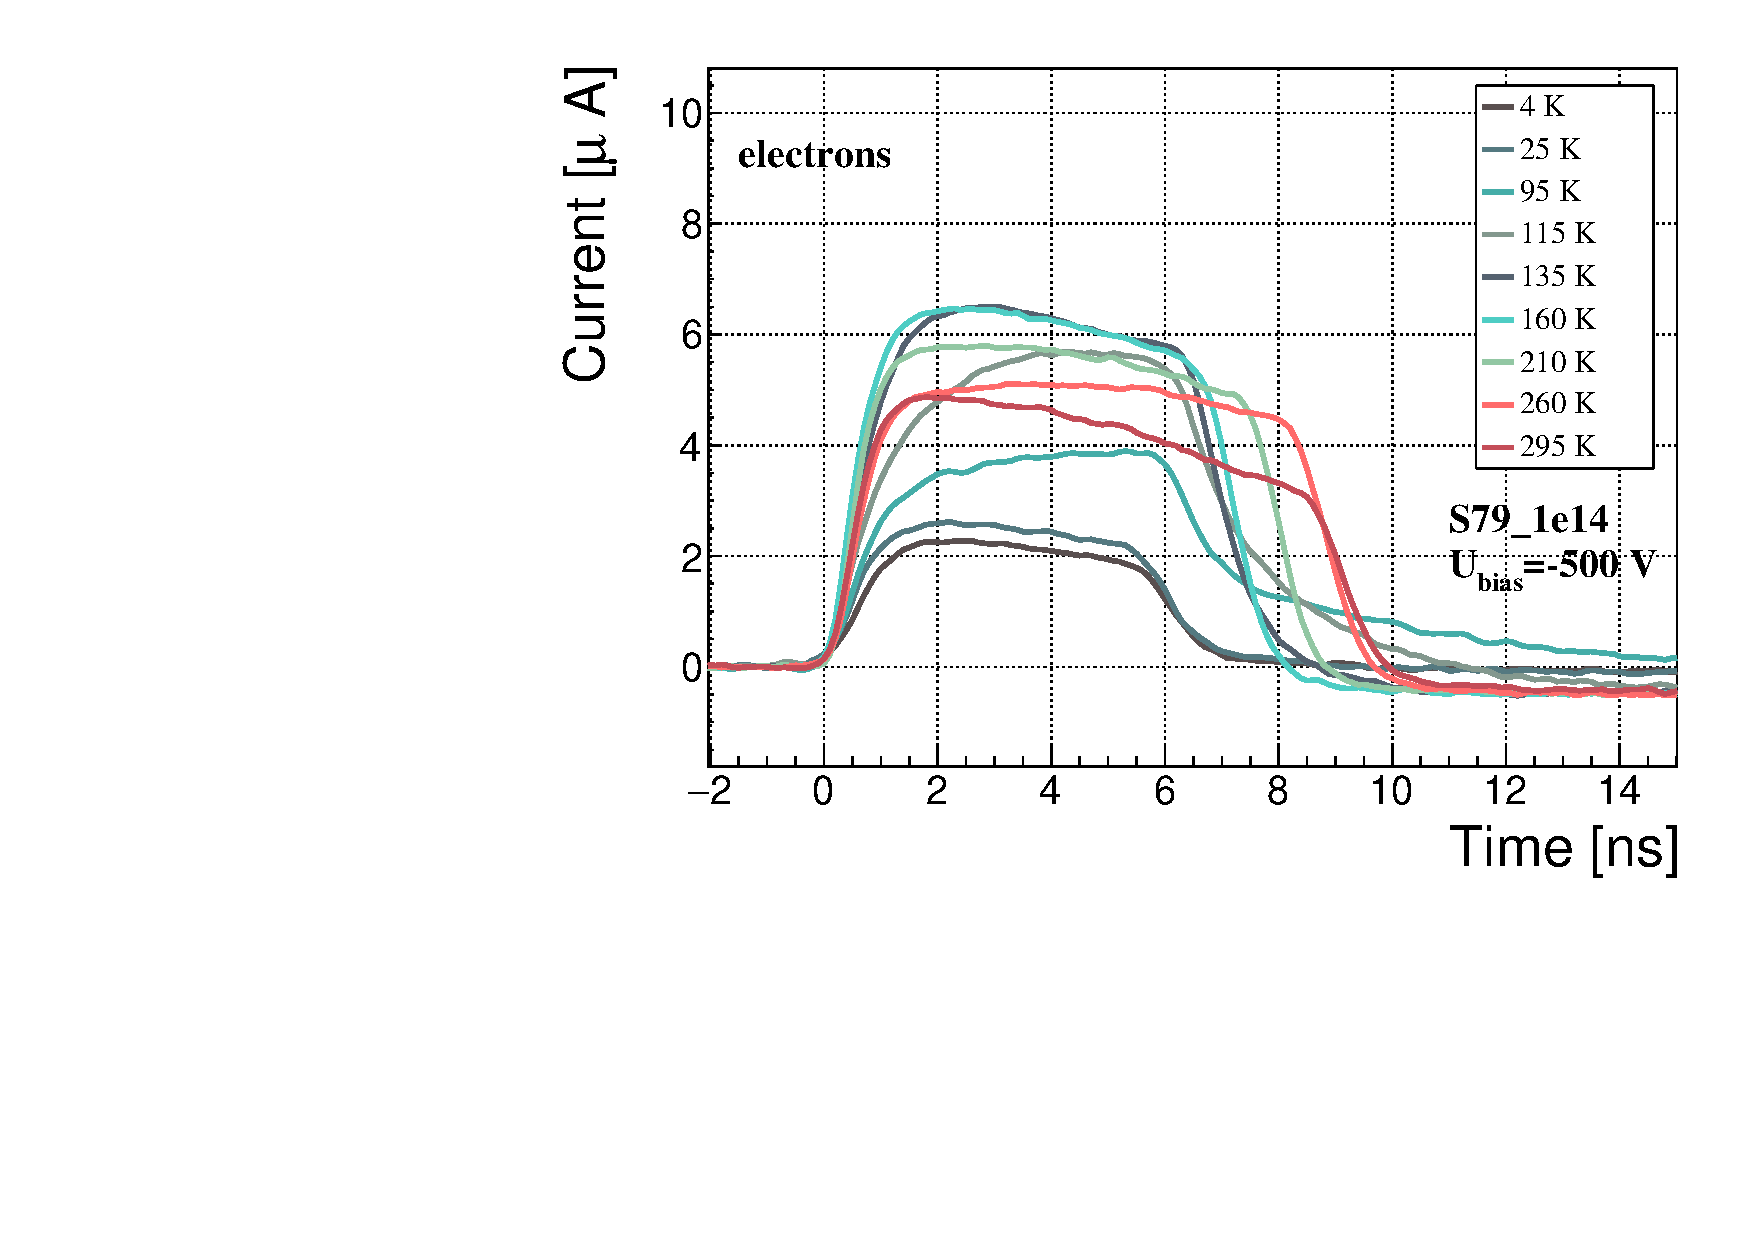
\includegraphics[width=0.47\textwidth]{scripts/plots/pulses/S79_1e14_elecs} \label{fig:S79plusAfter}} &
\subfloat{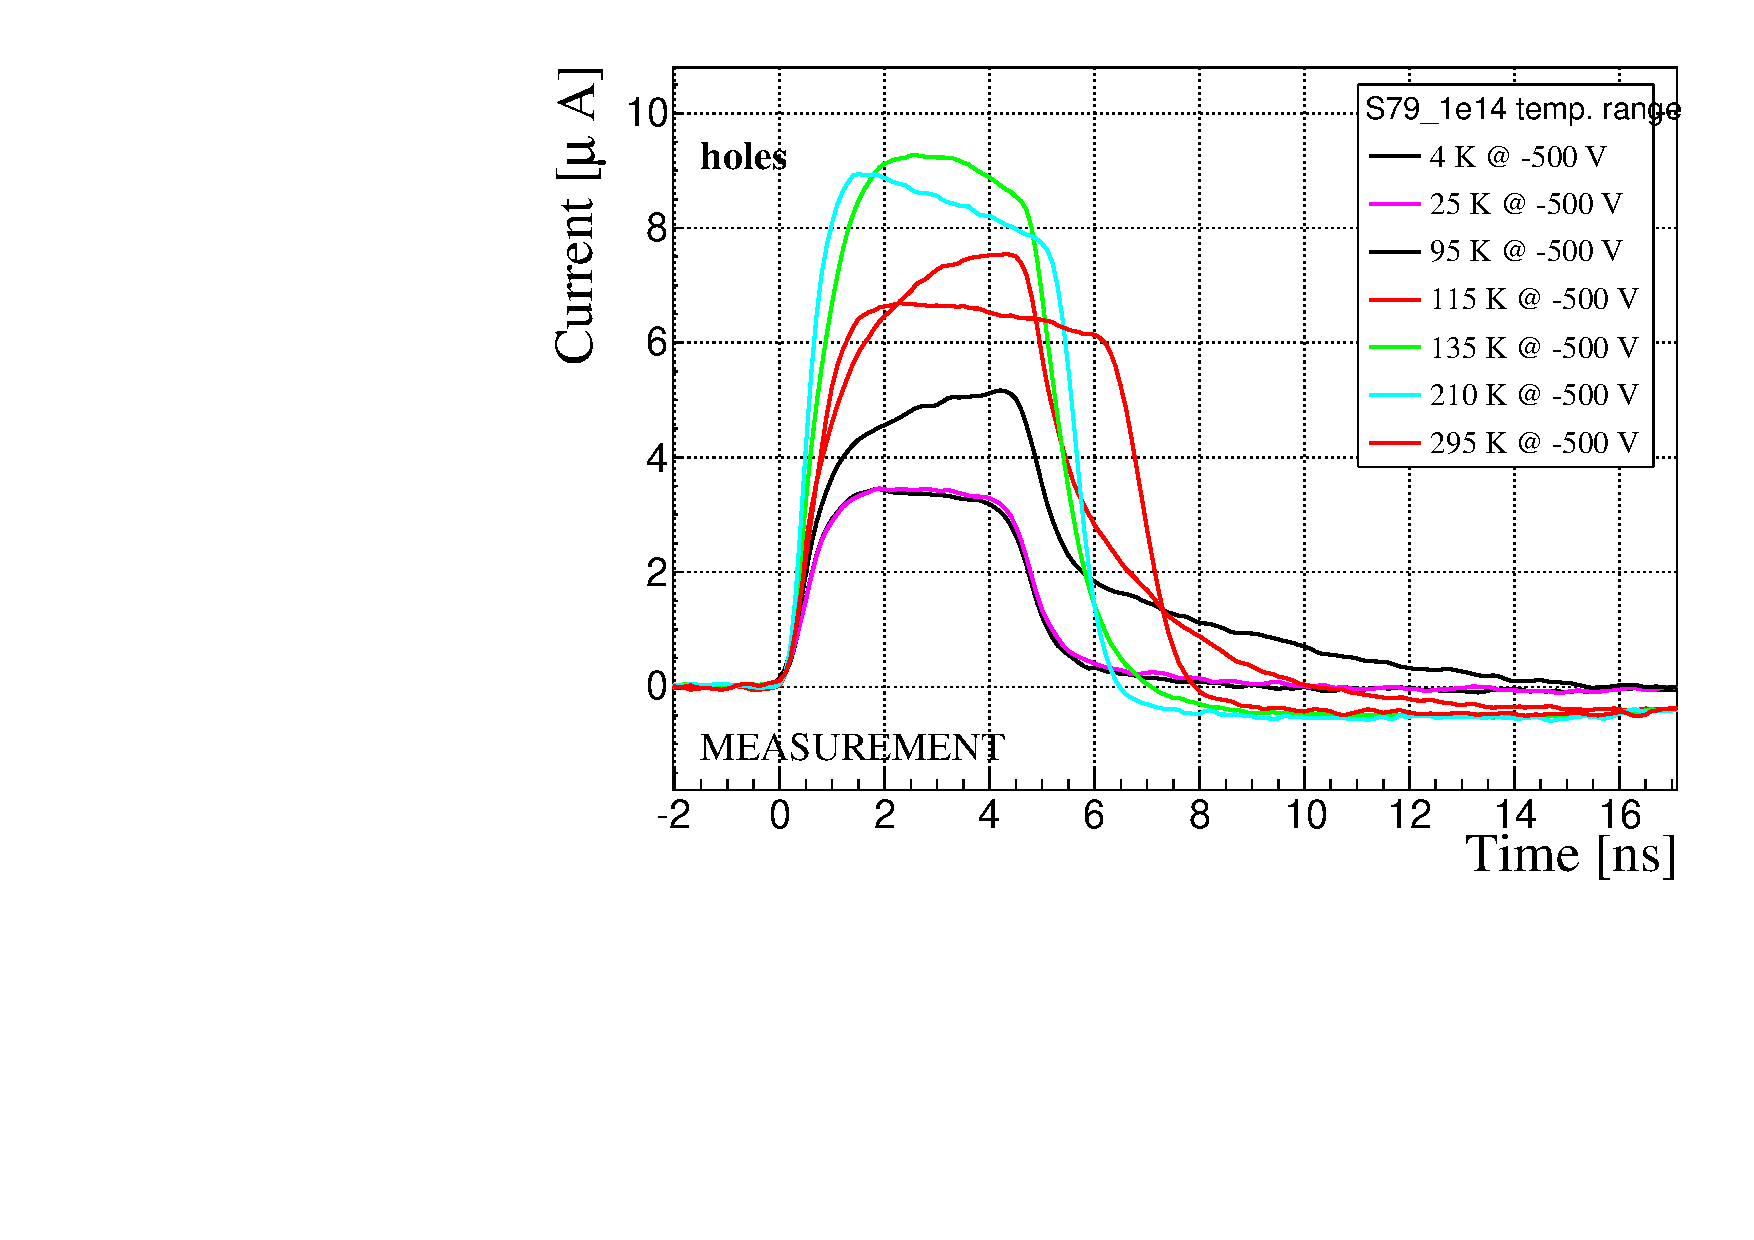
\includegraphics[width=0.47\textwidth]{scripts/plots/pulses/S79_1e14_holes}  \label{fig:S79minusAfter}} \\
\subfloat{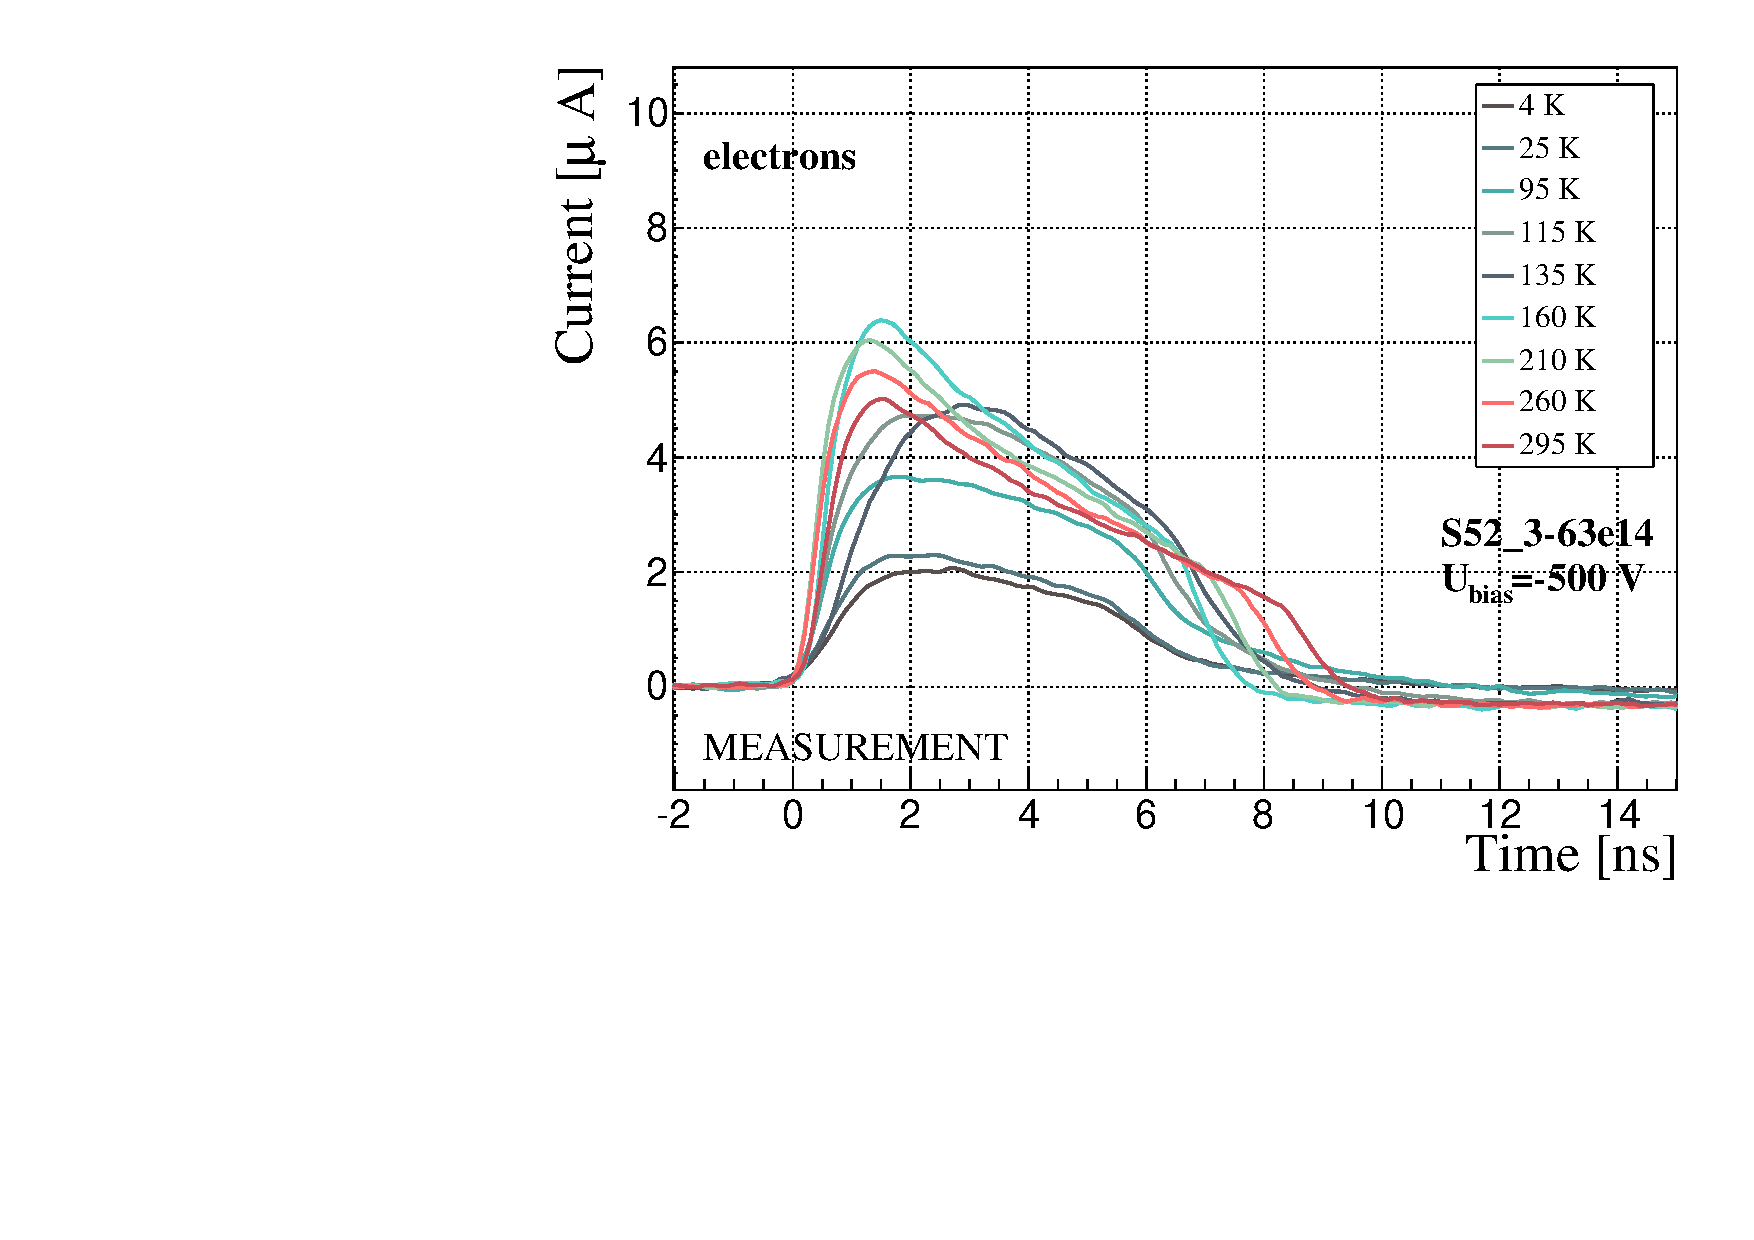
\includegraphics[width=0.47\textwidth]{scripts/plots/pulses/S52_3-63e14_elecs} \label{fig:S52plusAfter}} &
\subfloat{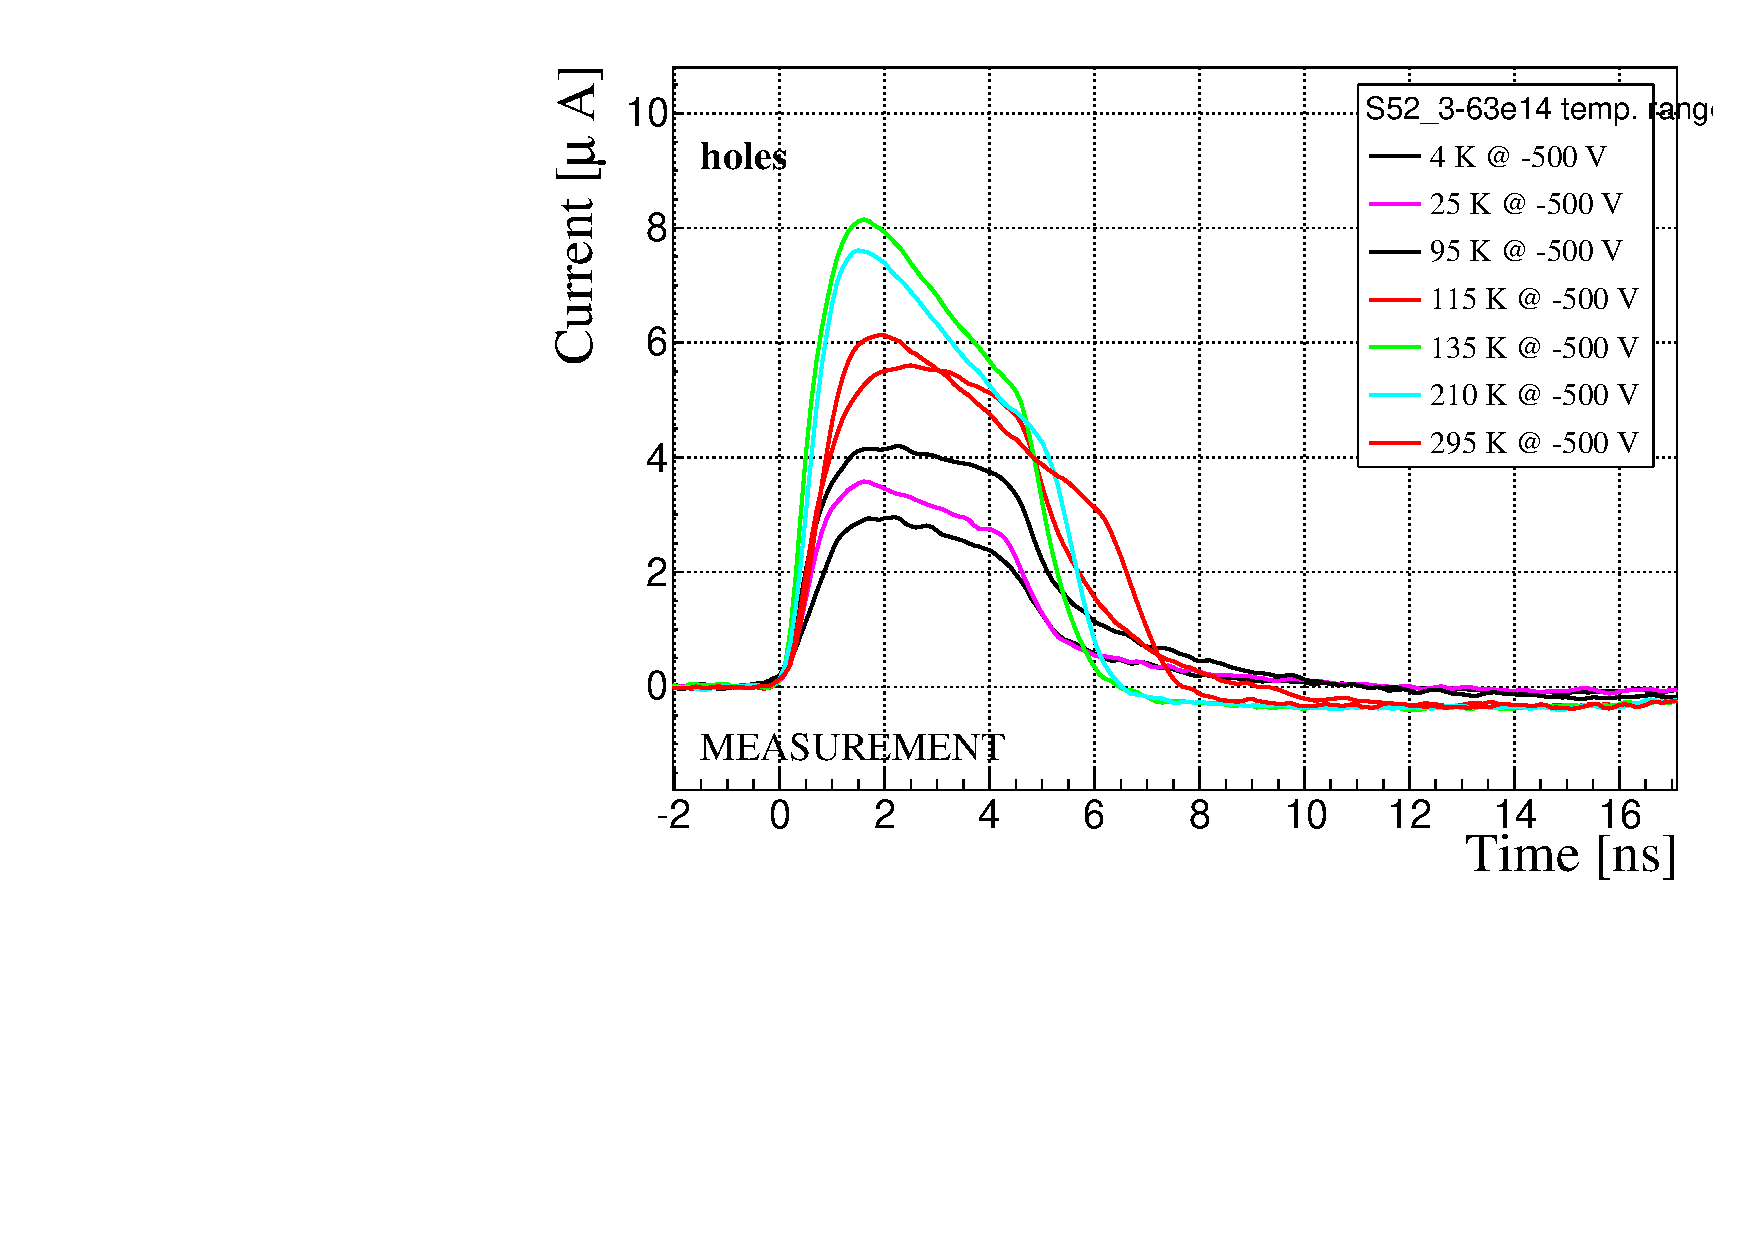
\includegraphics[width=0.47\textwidth]{scripts/plots/pulses/S52_3-63e14_holes}  \label{fig:S52minusAfter}}
\end{tabular}
\caption{After irradiation: several data points between 4~K and 295~K at a bias voltage of $\pm$500~V}
\label{fig:temppulsesAfter}
\end{figure}

A decaying exponential function was fitted to the decaying top at pulses at bias voltages of $\pm$400~V and $\pm$500~V across all temperatures excluding the transitional range between 75~K and 150~K. There was a spread of fitted values at individual temperature points, stemming from the fact that the pulses changed with time due to "polarisation". This counts as a systematic error. Therefore all four fitted values were averaged into one value representing the measurement at that temperature point. Figure~\ref{fig:lifetimevstemp} shows the fitted decay time constants for the five samples between 4~K and 295~K. In principle, the time constants should be infinite for a perfect and non-irradiated sample. Here a slightly decreasing top due to space charge was already successfully fitted with an exponential function, resulting in a time constant of the order of 200~s$^{-1}$. This is also why the spread is enormous. For the irradiated samples, the fit becomes increasingly more meaningful. As seen in the plot, the fitted values of the irradiated samples are fairly stable across all temperatures. There is a slight increase in the decay time constant of the S52 from $(6\pm0.5)$~s$^{-1}$ above 150~K to ($8.5\pm0.9$)~s$^{-1}$ below 75~K. On the other hand, this step is not observable in the S79 data. With only one sample exhibiting this behaviour, the effect is not significant enough. Judging by the data acquired, the samples would need to be irradiated to doses above $1\times10^{14}~\uppi~$cm$^{-2}$ to quantify this effect in detail. All things considered, this effect will not be regarded as significant for the scope of this thesis. Building on this assumption, the conclusion is that the signal decay time constant for irradiated sCVD diamond is constant across the temperature range between 4~K and 195~K, excluding the transitional range between 75~K and 150~K. 

Taking into account the conclusions above, all the values can be averaged into one decay constant. Figure~\ref{fig:lifetimevsdose} shows these values for all samples plotted against received $\uppi$ radiation dose. To estimate the carrier lifetime with respect to the radiation dose received, a similar model was used than that in section~\ref{sec:radlimit}. This model states that the inverse of the carrier lifetime is linearly decreasing with increasing radiation dose:
\begin{equation}
\label{eq:ltfactor}
\frac{1}{\tau} = \frac{1}{\tau_0}+k_{\tau}\cdot\Phi
\end{equation} 
\begin{equation}
\label{eq:ltfactor1}
\tau = \frac{\tau_0}{k_{\tau} \tau_0 \Phi + 1}
\end{equation} 
where $\tau_0$ is the lifetime for a non-irradiated sample (real lifetime, therefore of the order of 400~s$^{-1}$), $\tau$ is the lifetime of an irradiated sample, $\Phi$ is the received radiation dose and $k_{\tau}$ the lifetime degradation factor. For these data the fitted factor was equal to k$_{tau}=(3.6\pm0.8)\times10^{-16}~$s~cm$^2$~$\uppi_{300~MeV}^{-1}$. Using this factor, the steepness of the decay in the pulse shape with respect to radiation dose can be estimated. This can help when designing a system where current pulse shape is an important factor.
%introduce the kTau factor

\begin{figure}[!t]
%\centering
\begin{tabular}{cccc}
\subfloat[Carrier lifetime as a function of temperature]{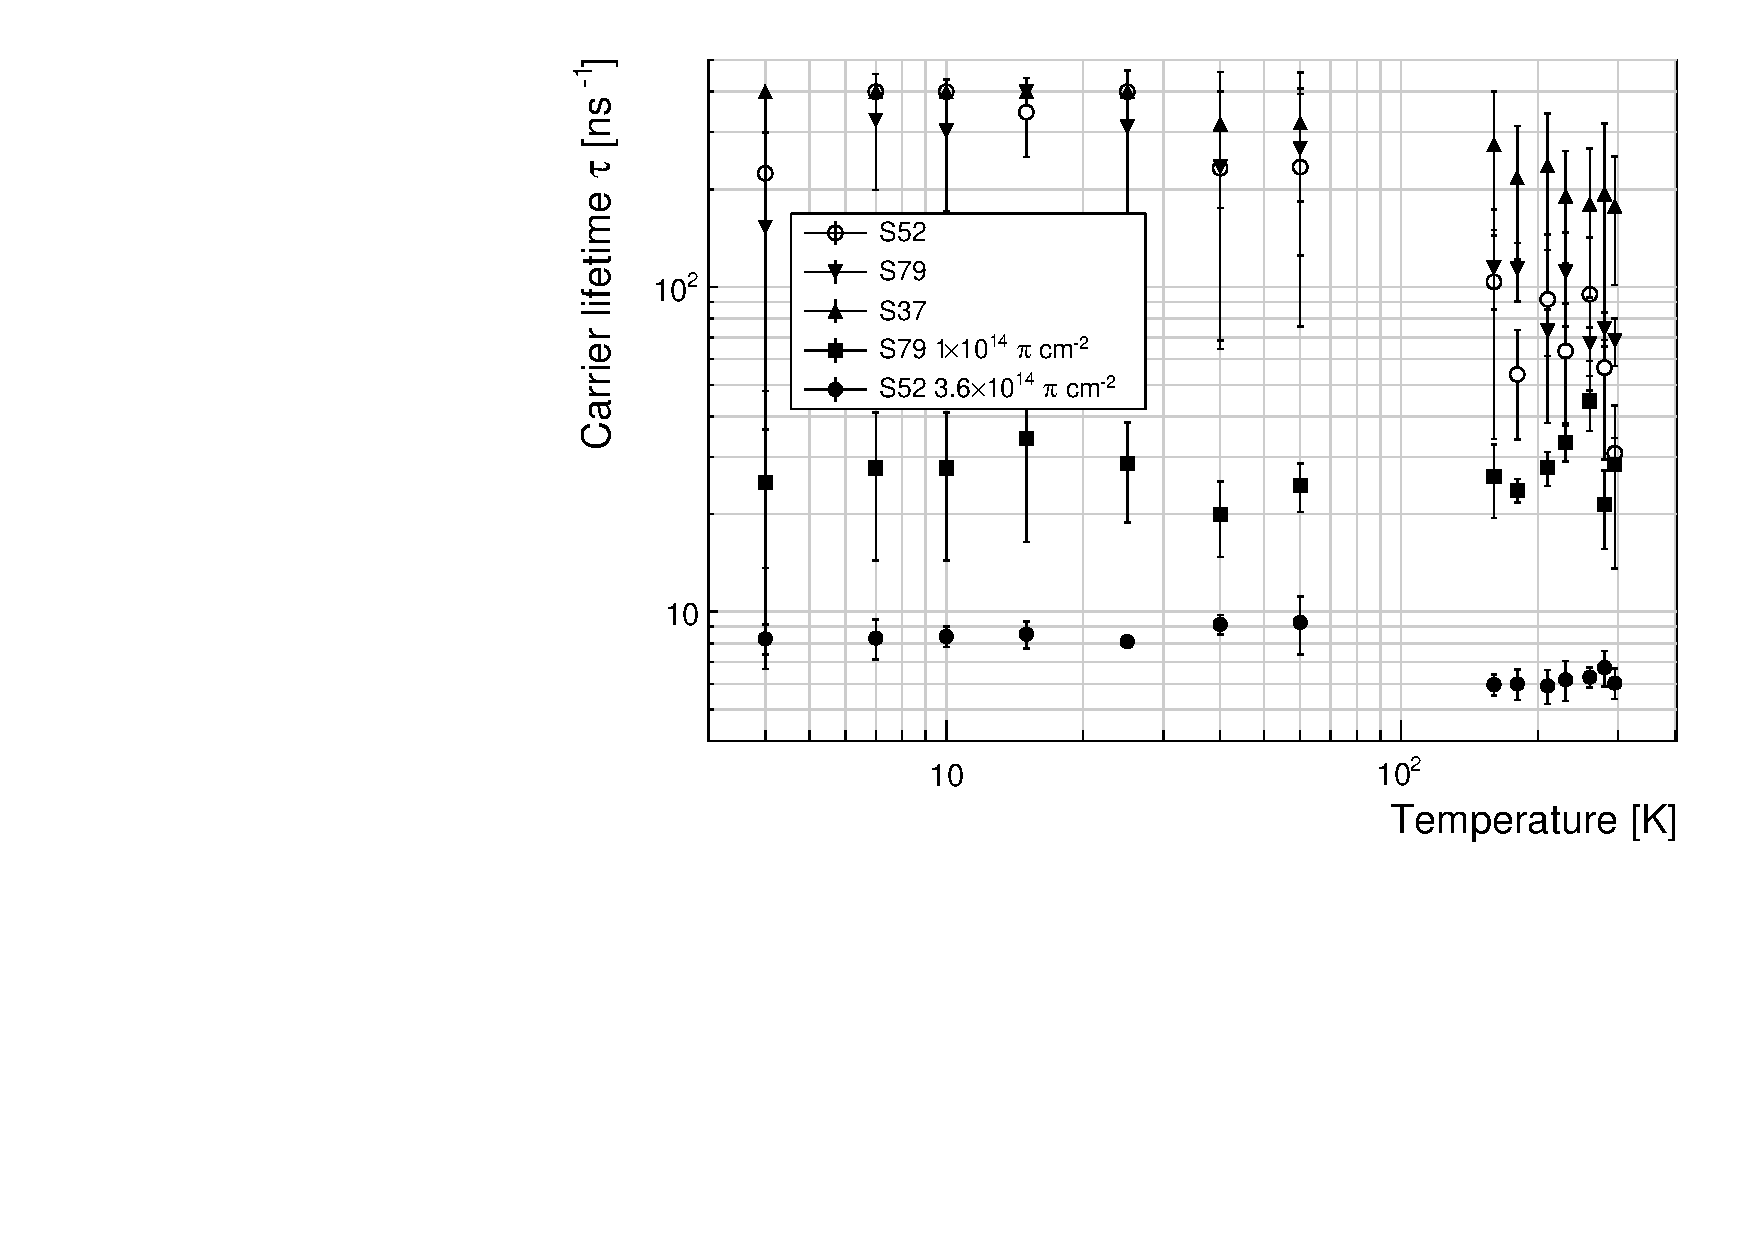
\includegraphics[width=0.45\textwidth]{scripts/plots/taunew/lifetimevstemp} \label{fig:lifetimevstemp}} &
\subfloat[Carrier lifetime averaged over all temperatures as a function of $\pi$ irradiation dose]{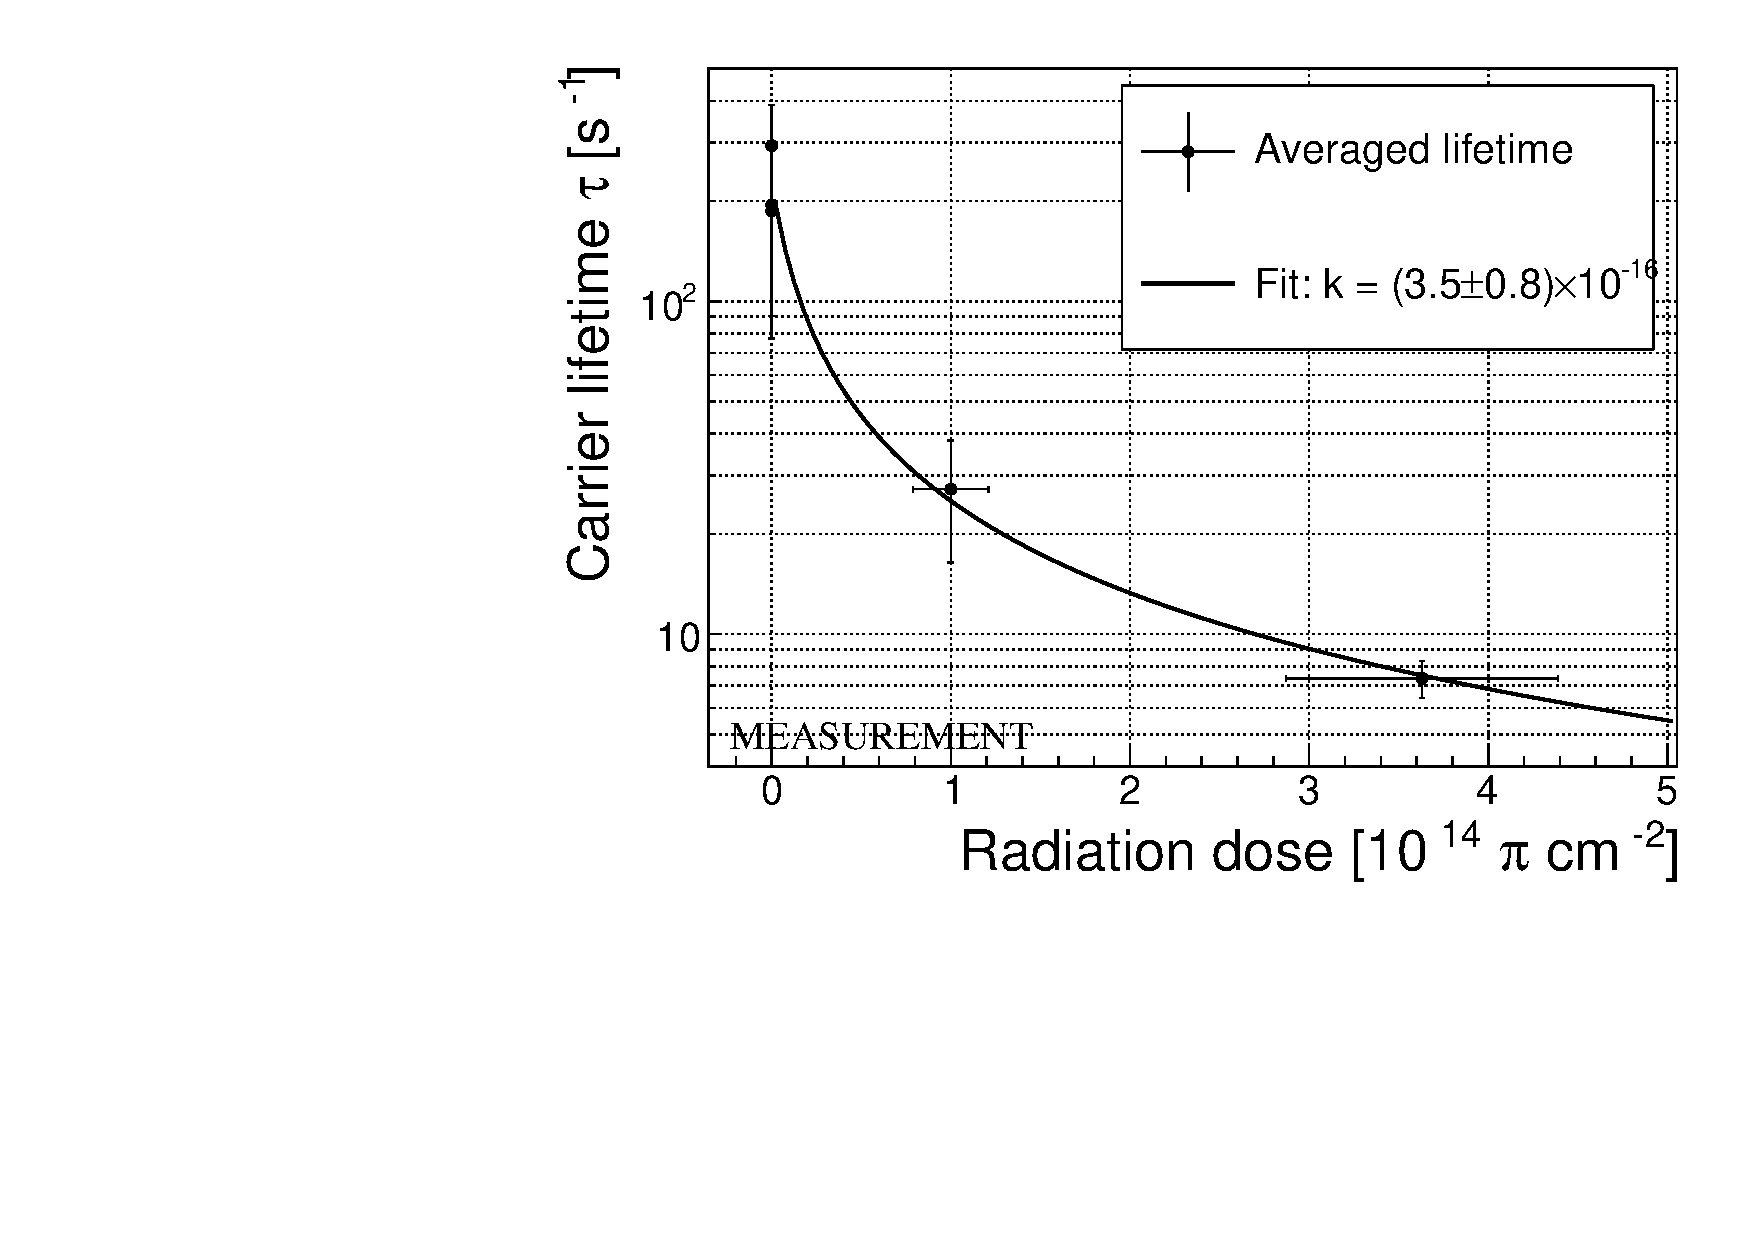
\includegraphics[width=0.45\textwidth]{scripts/plots/taunew/avglifetime}  \label{fig:lifetimevsdose}}
\end{tabular}
\caption{Charge carrier lifetime decreases with irradiation, but is stable across the range of temperatures between 4~K -- 75~K and 150~K -- 295~K.}
\end{figure}











% ---------------------------------------------------------------------------------------------------------------
%\clearpage
\section{Conclusion}
\label{sec:radlimit}
% ---------------------------------------------------------------------------------------------------------------
This chapter gave an overview of the capabilities and limitations of diamond as a particle detector. Three effects on diamond were studied -- noise, radiation and temperature, the focus being on the latter two. 

Two sCVD diamond detectors were irradiated with 300~MeV pions. They were tested alongside a non-irradiated sample to observe the changes in the ability to detect $\upalpha$, $\upbeta$ and $\upgamma$ radiation. Their charge collection efficiency was measured in a test beam facility using . The results were compared to the results from the RD42 collaboration and a DPA model provided by Karlsruhe Institute of Technology, Germany. A radiation damage factor $k=(3.2\pm1)\times10^{-18}$ was obtained. The data point did not fully overlap with the data provided by RD42 nor the model. However, the irradiation process and the low number of tested samples hold a relatively high statistical uncertainty. These results will also be fed into the existing pool of data in the RD42 collaboration, increasing the otherwise rather low number of measurement points of irradiated diamond samples. 

The next step was to test the long-term capabilities for $\upalpha$ detection. The shape of the ionisation profile was investigated to determine the behaviour of the charge carriers in the irradiated diamond. An exponential decay was observed in the pulse, proving that there are charge traps in the bulk that were created during irradiation.  Then a long-term stability test was carried out. The results show that the irradiated diamond detectors do not provide a stable and reliable long-term measurement of $\upalpha$ particles. Presumably this is due to a space-charge build-up in the bulk, which changes the electric field, affecting the charge carriers. A procedure to improve the pulse shape using $\upbeta$ and $\upgamma$ radiation was proposed.

Finally, the diamond sensors were cooled down to temperatures between 4~K and 295~K. Their response to $\upalpha$ particles was observed. The results of the non-irradiated and irradiated samples were compared. The effect of reduction for the number of drifting charges due to exciton recombination was observed in both sets of data. The second set had a superimposed effect of charge trapping during the drift, which was represented by an exponential decay in the signal. The decay time constant did not change with temperature. Therefore all temperature points for individual samples were averaged and the decay time constants were plotted against the received radiation dose. A damage factor equal to $k=(3.6\pm0.8)\times10^{-16}$ for non-primed diamonds was defined.



% ---------------------------- comment out when compiling the full document -------------------
\end{document}
% ---------------------------------------------------------------------------------------------------------------
